%% Para utilizar este template siga o tutorial disponível em http://www.biblioteca.ufc.br/images/arquivos/instrucoes_modelos/tutorial_sharelatex.pdf

%%%%%%%%%%%%%%%%%%%%%%%%%%%%%%%%%%%%%%%%%%%%%%%%%%%%%%%
%% Você dever criar uma conta no ShareLatex. Depois, %%
%% vá nas opções no canto esquerdo superior da tela  %%
%% e clique em "Copiar Projeto". Dê um novo nome pa- %%
%% ra o projeto.                                     %%
%%                                                   %%
%% Os principais desenvolvedores deste template são: %%
%%                                                   %%
%%            Ednardo Moreira Rodrigues              %%
%%     (Doutorando em Engenharia Elétrica - UFC)     %%
%%                      &                            %%
%%            Alan Batista de Oliveira               %%
%%     (Graduando em Engenharia Elétrica - UFC)      %%
%%                                                   %%
%% Revisão:                                          %%
%%                                                   %%
%% - Eliene Maria Vieira de Moura;                   %%
%% - Francisco Edvander Pires Santos;                %%
%% - Izabel Lima dos Santos;                         %%
%% - Juliana Soares Lima;                            %%
%% - Kalline Yasmin Soares Feitosa.                  %%
%%                                                   %%
%% Grande parte do trabalho foi adaptado do template %%
%% da UECE elaborado por:                            %%
%% Thiago Nascimento  (UECE)                         %%
%% Project available on:                             %%
%% https://github.com/thiagodnf/uecetex2             %%
%%                                                   %%
%% "Dúvidas, esclarecimentos ou sugestões podem ser  %%
%% enviadas para o e-mail da Comissão de Serviços da %%
%% Biblioteca Universitária: csbu@ufc.br."           %%
%%                                                   %%
%%%%%%%%%%%%%%%%%%%%%%%%%%%%%%%%%%%%%%%%%%%%%%%%%%%%%%%                                  %%                                                   %%
%% Alterado em 2017 para ser base dos trabalhos de   %%
%% conclusão de curso da Enegenahria Elétrica        %%
%% da UFPI.                                          %%
%% Prof. José Maria Pires de Menezes Jr.             %%
%%                                                   %%
%%%%%%%%%%%%%%%%%%%%%%%%%%%%%%%%%%%%%%%%%%%%%%%%%%%%%%%

\documentclass[        
    a4paper,          % Tamanho da folha A4
    12pt,             % Tamanho da fonte 12pt
    chapter=TITLE,    % Todos os capitulos devem ter caixa alta
    section=Title,    % Todas as secoes devem ter caixa alta somente na primeira letra
    subsection=Title, % Todas as subsecoes devem ter caixa alta somente na primeira letra
    oneside,          % Usada para impressao em apenas uma face do papel
    english,          % Hifenizacoes em ingles
    spanish,          % Hifenizacoes em espanhol
    brazil,           % Ultimo idioma eh o idioma padrao do documento
    %fleqn             % Coloca as equações alinhadas a esquerda
]{abntex2}


% Para utilizar este template siga o tutorial disponível em http://www.biblioteca.ufc.br/images/arquivos/instrucoes_modelos/tutorial_sharelatex.pdf

%%%%%%%%%%%%%%%%%%%%%%%%%%%%%%%%%%%%%%%%%%%%%%%%%%%%%%%
%%      Para começar a usar este template, primeiro, %%
%% você dever criar uma conta no ShareLatex. Depois, %%
%% vá nas opções no canto esquerdo superior da tela  %%
%% e clique em "Copiar Projeto". Dê um novo nome pa- %%
%% ra o projeto.                                     %%
%%                                                   %%
%% Os principais desenvolvedores deste template são: %%
%%                                                   %%
%%             Ednardo Moreira Rodrigues             %%
%%     (Doutorando em Engenharia Elétrica - UFC)     %%
%%                      &                            %%
%%            Alan Batista de Oliveira               %%
%%     (Graduando em Engenharia Elétrica - UFC)      %%
%%                                                   %%
%% Revisão:                                          %%
%%                                                   %%
%% - Eliene Maria Vieira de Moura;                   %%
%% - Francisco Edvander Pires Santos;                %%
%% - Izabel Lima dos Santos;                         %%
%% - Juliana Soares Lima;                            %%
%% - Kalline Yasmin Soares Feitosa.                  %%
%%                                                   %%
%% Grande parte do trabalho foi adaptado do template %%
%% da UECE elaborado por:                            %%
%% Thiago Nascimento  (UECE)                         %%
%% Project available on:                             %%
%% https://github.com/thiagodnf/uecetex2             %%
%%                                                   %%
%% "Dúvidas, esclarecimentos ou sugestões podem ser  %%
%% enviadas para o e-mail da Comissão de Serviços da %%
%% Biblioteca Universitária: csbu@ufc.br."           %%
%%                                                   %%
%%%%%%%%%%%%%%%%%%%%%%%%%%%%%%%%%%%%%%%%%%%%%%%%%%%%%%%

% Importações de pacotes
\usepackage[utf8]{inputenc}                         % Acentuação direta
\usepackage[T1]{fontenc}                            % Codificação da fonte em 8 bits
\usepackage{graphicx}                               % Inserir figuras
\usepackage{amsfonts, amssymb, amsmath}             % Fonte e símbolos matemáticos
\usepackage{booktabs}                               % Comandos para tabelas
\usepackage{verbatim}                               % Texto é interpretado como escrito no documento
\usepackage{multirow, array}                        % Múltiplas linhas e colunas em tabelas
\usepackage{indentfirst}                            % Endenta o primeiro parágrafo de cada seção.
\usepackage{listings}                               % Utilizar codigo fonte no documento
\usepackage{xcolor}
\usepackage{microtype}                              % Para melhorias de justificação?
\usepackage[portuguese,ruled,lined]{algorithm2e}    % Escrever algoritmos
\usepackage{algorithmic}                            % Criar Algoritmos  
%\usepackage{float}                                  % Utilizado para criação de floats
\usepackage{amsgen}
\usepackage{lipsum}                                 % Usar a simulação de texto Lorem Ipsum
%\usepackage{titlesec}                               % Permite alterar os títulos do documento
\usepackage{tocloft}                                % Permite alterar a formatação do Sumário
\usepackage{etoolbox}                               % Usado para alterar a fonte da Section no Sumário
\usepackage[nogroupskip,nonumberlist]{glossaries}                % Permite fazer o glossario
\usepackage[font=singlespacing]{caption}            % Altera o comportamento da tag caption

%\usepackage[alf, abnt-emphasize=bf, recuo=0cm, abnt-etal-cite=2, abnt-etal-list=0, abnt-etal-text=it]{abntex2cite}  % Citações padrão ABNT

\usepackage[alf, abnt-emphasize=bf, recuo=0cm, abnt-etal-cite=3, abnt-etal-list=3, abnt-etal-text=it]{abntex2cite}  % Citações padrão ABNT
%\usepackage[bottom]{footmisc}                      % Mantém as notas de rodapé sempre na mesma posição
%\usepackage{times}                                 % Usa a fonte Times
\usepackage{mathptmx}                               % Usa a fonte Times New Roman										
%\usepackage{lmodern}                               % Usa a fonte Latin Modern
%\usepackage{subfig}                                % Posicionamento de figuras
%\usepackage{scalefnt}                              % Permite redimensionar tamanho da fonte
%\usepackage{color, colortbl}                       % Comandos de cores
%\usepackage{lscape}                                % Permite páginas em modo "paisagem"
%\usepackage{ae, aecompl}                           % Fontes de alta qualidade
%\usepackage{picinpar}                              % Dispor imagens em parágrafos
%\usepackage{latexsym}                              % Símbolos matemáticos
%\usepackage{upgreek}                               % Fonte letras gregas
\usepackage{appendix}                               % Gerar o apendice no final do documento
\usepackage{paracol}                                % Criar paragrafos sem identacao
\usepackage{lib/ufctex}		                        % Biblioteca com as normas da UFC para trabalhos academicos
\usepackage{pdfpages}                               % Incluir pdf no documento
\usepackage{amsmath}                                % Usar equacoes matematicas
\usepackage{cancel}
\usepackage{bm}
\usepackage{enumitem}
\newcommand\numberthis{\addtocounter{equation}{1}\tag{\theequation}}
%\usepackage{listingsutf8}
\usepackage[brazil]{babel}

% Organiza e gera a lista de abreviaturas, simbolos e glossario
\makeglossaries

% Gera o Indice do documento
\makeindex


%%%%%%%%%%%%%%%%%%%%%%%%%%%%%%%%%%%%%%%%%%%%%%%%%%%%%
%%          Configuracoes do ufctex                %%
%%%%%%%%%%%%%%%%%%%%%%%%%%%%%%%%%%%%%%%%%%%%%%%%%%%%%

% Opcoes disponiveis

\trabalhoacademico{tccgraduacao}
%\trabalhoacademico{tccespecializacao}
%\trabalhoacademico{dissertacao}
%\trabalhoacademico{tese}

% Define se o trabalho eh uma qualificacao
% Coloque 'nao' para versao final do trabalho

\ehqualificacao{nao}

% Remove as bordas vermelhas e verdes do PDF gerado
% Coloque 'sim' pare remover

\removerbordasdohyperlink{sim} 

% Adiciona a cor Azul a todos os hyperlinks

\cordohyperlink{nao}

%%%%%%%%%%%%%%%%%%%%%%%%%%%%%%%%%%%%%%%%%%%%%%%%%%%%%
%%          Informação sobre a IES                 %%
%%%%%%%%%%%%%%%%%%%%%%%%%%%%%%%%%%%%%%%%%%%%%%%%%%%%%

\ies{Universidade Federal do Piauí}
\iessigla{UFPI}
\centro{Centro de Tecnologia}

%%%%%%%%%%%%%%%%%%%%%%%%%%%%%%%%%%%%%%%%%%%%%%%%%%%%%
%%        Informação para TCC de Graduacao %%
%%%%%%%%%%%%%%%%%%%%%%%%%%%%%%%%%%%%%%%%%%%%%%%%%%%%%

\graduacaoem{Engenharia Elétrica}
\habilitacao{bacharel} % Pode colocar tambem 'licenciada'

%%%%%%%%%%%%%%%%%%%%%%%%%%%%%%%%%%%%%%%%%%%%%%%%%%%%%
%%     Informação para TCC de Especializacao       %%
%%%%%%%%%%%%%%%%%%%%%%%%%%%%%%%%%%%%%%%%%%%%%%%%%%%%%

% \especializacaoem{Descargas Atmosféricas}

%%%%%%%%%%%%%%%%%%%%%%%%%%%%%%%%%%%%%%%%%%%%%%%%%%%%%
%%         Informação para Dissertacao             %%
%%%%%%%%%%%%%%%%%%%%%%%%%%%%%%%%%%%%%%%%%%%%%%%%%%%%%

% \programamestrado{Programa de Pós-Graduação em Xxxxxxx}
% \nomedomestrado{Mestrado Acadêmico em Xxxxxxx}
% \mestreem{Engenharia Xxxxxx}
% \areadeconcentracaomestrado{Engenharia Xxxxxx}

%%%%%%%%%%%%%%%%%%%%%%%%%%%%%%%%%%%%%%%%%%%%%%%%%%%%%
%%               Informação para Tese              %%
%%%%%%%%%%%%%%%%%%%%%%%%%%%%%%%%%%%%%%%%%%%%%%%%%%%%%

% \programadoutorado{Programa de Pós-Graduação em Xxxxxx}
% \nomedodoutorado{Doutorado em Xxxxxxx}
% \doutorem{Engenharia Xxxxxx}
% \areadeconcentracaodoutorado{Engenharia Xxxxxxx}

%%%%%%%%%%%%%%%%%%%%%%%%%%%%%%%%%%%%%%%%%%%%%%
%%  Informacoes relacionadas ao trabalho     %%
%%%%%%%%%%%%%%%%%%%%%%%%%%%%%%%%%%%%%%%%%%%%%%

\autor{HÄNDEL MATEUS CARVALHO SARMENTO}
\titulo{CONTROLE DE VELOCIDADE DE UM ROBÔ MICROMOUSE}
\data{2026}
\local{Teresina}

% Exemplo: \dataaprovacao{01 de Janeiro de 2012}
\dataaprovacao{}

%%%%%%%%%%%%%%%%%%%%%%%%%%%%%%%%%%%%%%%%%%%%%
%%     Informação sobre o Orientador       %%
%%%%%%%%%%%%%%%%%%%%%%%%%%%%%%%%%%%%%%%%%%%%%

\orientador{Prof. Dr. Otacílio da Mota Almeida}
\orientadories{Universidade Federal do Piauí (UFPI)}
\orientadorcentro{Centro de Tecnologia (CT)}
\orientadorfeminino{nao} % Coloque 'sim' se for do sexo feminino

%%%%%%%%%%%%%%%%%%%%%%%%%%%%%%%%%%%%%%%%%%%%%
%%      Informação sobre o Co-orientador   %%
%%%%%%%%%%%%%%%%%%%%%%%%%%%%%%%%%%%%%%%%%%%%%

% Deixe o nome do coorientador em branco para remover do documento

\coorientador{}
\coorientadories{Universidade Co-orientador (SIGLA)}
\coorientadorcentro{Centro do Co-orientador (SIGLA)}
\coorientadorfeminino{nao} % Coloque 'sim' se for do sexo feminino

%%%%%%%%%%%%%%%%%%%%%%%%%%%%%%%%%%%%%%%%%%%%%
%%      Informação sobre a banca           %%
%%%%%%%%%%%%%%%%%%%%%%%%%%%%%%%%%%%%%%%%%%%%%

% Atenção! Deixe o nome do membro da banca para remover da folha de aprovacao

% Exemplo de uso:
% \membrodabancadois{Prof. Dr. Fulano de Tal}
% \membrodabancadoisies{Universidade Federal do Ceará - UFC}

\membrodabancadois{Prof. XXXXXXXXXXXXXX}
\membrodabancadoiscentro{Centro de Tecnologia (CT)}
\membrodabancadoisies{Universidade Federal do Piauí (UFPI)}
\membrodabancatres{Prof. YYYYYYYYY}
\membrodabancatrescentro{Centro de Tecnologia (CT)}
\membrodabancatresies{Centro Universitário Maurício de Nassau (UNINASSAU)}
%\membrodabancaquatro{Prof. Dr. Xxxxxxx Xxxxxx Xxxxxxx}
%\membrodabancaquatrocentro{Centro de Ciências e Tecnologia (CCT)}
%\membrodabancaquatroies{Universidade do Membro da Banca Quatro (SIGLA)}
%\membrodabancacinco{Prof. Dr. Xxxxxxx Xxxxxx Xxxxxxx}
%\membrodabancacincocentro{Teste}
%\membrodabancacincoies{Universidade do Membro da Banca Cinco (SIGLA)}
%\membrodabancaseis{Prof. Dr. Xxxxxxx Xxxxxx Xxxxxxx}
%\membrodabancaseiscentro{}
%\membrodabancaseisies{Universidade do Membro da Banca Seis (SIGLA)}

\begin{document}	

	% Elementos pré-textuais
	\imprimircapa
	\imprimirfolhaderosto{}
	\imprimirfichacatalografica{elementos-pre-textuais/ficha-catalografica}
	%\imprimirerrata{elementos-pre-textuais/errata}
	% \imprimirfolhadeaprovacao
	\imprimirdedicatoria{elementos-pre-textuais/dedicatoria}
	\imprimiragradecimentos{elementos-pre-textuais/agradecimentos}
	\imprimirepigrafe{elementos-pre-textuais/epigrafe}
	\imprimirresumo{elementos-pre-textuais/resumo}
	\imprimirabstract{elementos-pre-textuais/abstract}
	\imprimirlistadeilustracoes
	\imprimirlistadetabelas
	%\imprimirlistadequadros
	%\imprimirlistadealgoritmos
	%\imprimirlistadecodigosfonte
	\imprimirlistadeabreviaturasesiglas
	% \imprimirlistadesimbolos{elementos-pre-textuais/lista-de-simbolos}   
	\imprimirsumario
	
	%Elementos textuais
	\textual
	\chapter{Introdução} \label{cap:introducao}
\setcounter{table}{0}
    A ideia de um robô solucionador de labirintos surge da década de 50 do século passado e foi concebido já como um robô autônomo, isto é, sem interferência humana no processo de pilotagem. 
    
    As competições de robôs capazes de resolver labirintos, popularmente chamados de \textit{micromouse}, por sua vez, datam da década de 70, quando foram lançados como competição do \gls{IEEE}, conforme mostrado em \citeonline{day1979amazing}. Estas competições até hoje são muito populares na Europa. Em países como o Reino Unido se destaca a \textit{UK micromouse}, em Portugal a \textit{Micromouse Portuguese Contest} e no Japão a \textit{all japan micromouse robot competition}. Este último é referência mundial nesse quesito e seus competidores são referências pelas mais diversas tecnologias empregadas, diferentes técnicas de aperfeiçoamento e diminutos tempos com que conseguem resolver e percorrer complexos labirintos \cite{borges2013micromouse}.

    A competição, resumidamente, consiste em resolver um labirinto, dividido em células, até encontrar o seu centro, partindo de um dos seus cantos, no menor tempo possível e, sempre, de forma autônoma, ou seja, os projetistas não podem operar o robô durante o percurso. 
    
    A seguir são listadas exemplos de regras para o caso japonês, conforme encontrado em \citeonline{micromouse-rules-japan-2023}.

    \begin{itemize}
        \item O \textit{Micromouse} deve ser autossuficiente. Não é permitida a utilização de fontes de energia baseadas em combustão.
        \item Nenhum componente de hardware ou software do \textit{Micromouse} pode ser adicionado, removido, substituído ou modificado pelo operador durante a competição. Entretanto, pequenos reparos e ajustes são permitidos.
        \item O \textit{Micromouse} não deve saltar, escalar, danificar ou romper as paredes do labirinto.
        \item O labirinto deve ser composto por células unitárias de $9\,\text{cm} \times 9\,\text{cm}$, sendo que seu tamanho total não pode exceder $32 \times 32$ células. A altura das paredes de cada célula deve ser de $2,5\,\text{cm}$ e sua espessura de $0,6\,\text{cm}$ (Figura \ref{fig:celulas-labirinto}).
        \item O ponto de partida do labirinto localiza-se em um dos quatro cantos, sendo a orientação inicial definida no sentido horário. O ponto de chegada consiste em uma área retangular previamente determinada (Figura \ref{fig:labirinto-micromouse-japao}).
        \item Não é permitido ao operador inserir qualquer informação sobre o labirinto no \textit{Micromouse} após a divulgação do percurso.
        \item Considera-se que um \textit{Micromouse} concluiu o labirinto quando todas as partes de sua estrutura estiverem completamente inseridas na área de chegada. 
    \end{itemize}

    \begin{figure}[htb]
        \centering
        \Caption{\label{fig:celulas-labirinto} Formato da célula do labirinto}
        \UFCfig{}{
            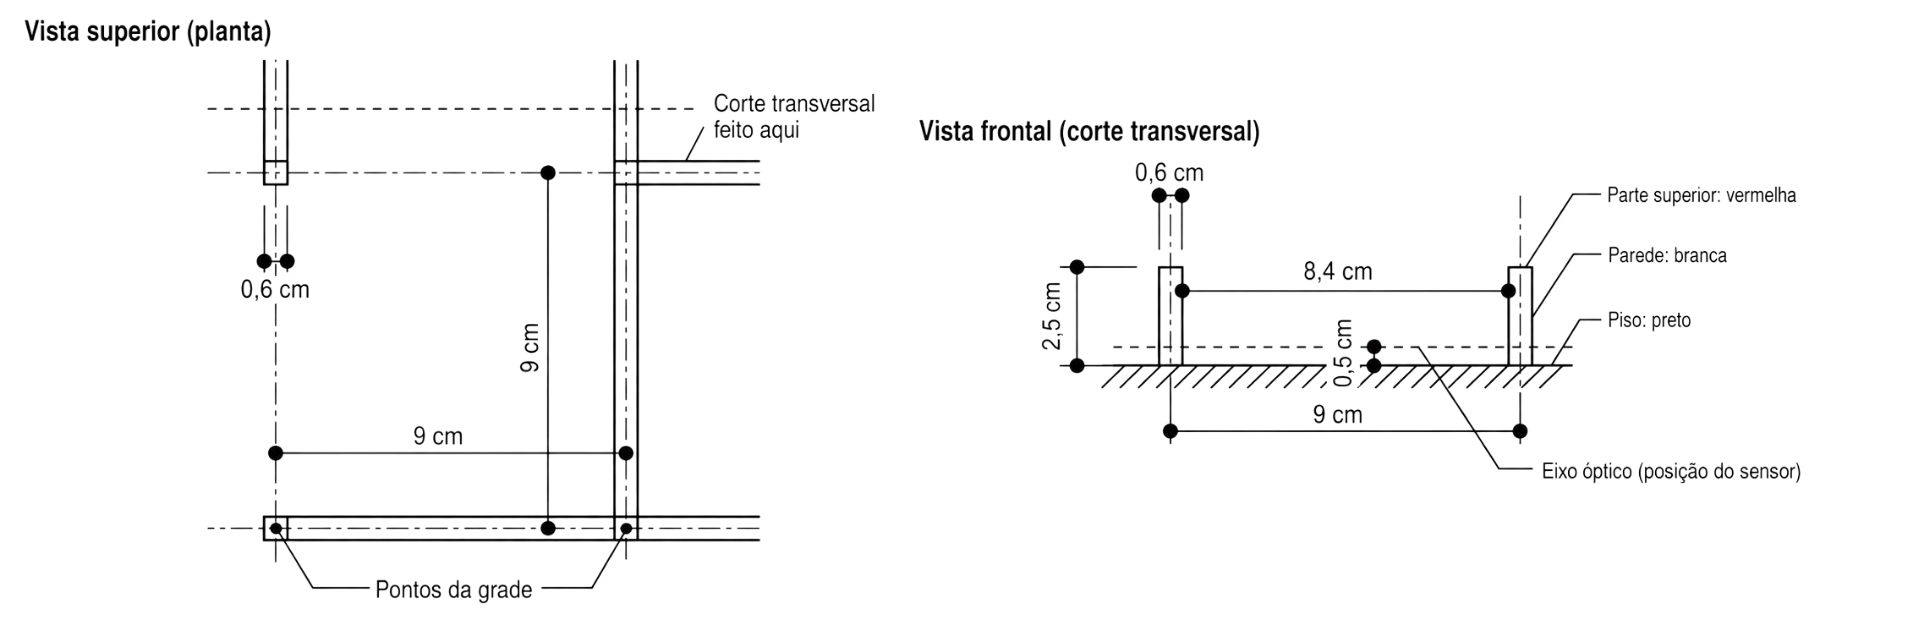
\includegraphics[width=12cm]{figuras/introducao/celula-labirinto-japao.png}
        }{
            \Fonte{Adaptado de \citeonline{micromouse-rules-japan-2023}}
        }	
    \end{figure}

    \begin{figure}[htb]
        \centering
        \Caption{\label{fig:labirinto-micromouse-japao} Labirinto do \textit{All Japan Micromouse Robot Competition}}
        \UFCfig{}{
            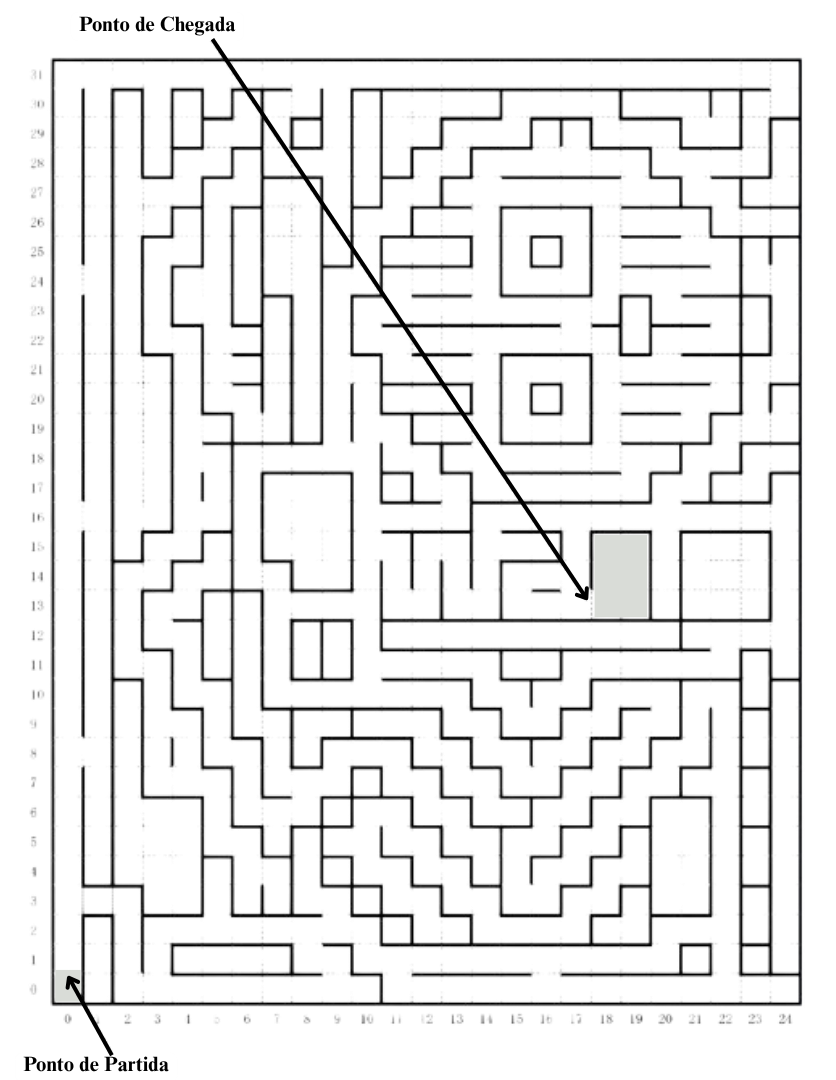
\includegraphics[width=7cm]{figuras/introducao/labirinto-japao.png}
        }{
            \Fonte{Adaptado de \citeonline{micromouse-rules-japan-2023}}
        }	
    \end{figure}

    Por já estar consolidado como um desafio dentro das engenharias, diversas abordagens são feitas ao redor do tópico do robô \textit{micromouse}. 
    
    Em \citeonline{su-et-al-2013} faz-se a implementação de uma versão simulada do comportamento do robô nos ambientes MATLAB/SIMULINK a fim de analisar questões relativas à resolução de labirinto, planejamento de trajetória e, também, técnicas de controle no contexto da cinemática diferencial do \textit{micromouse}.

    Já em \citeonline{micromouse-kit-educational} trabalha-se a implementação prática do robô a partir de um kit educacional desenvolvido em contexto escolar a fim de baratear os custor de uso quando comparados aos robôs comerciais. O referido kit conta com um microcontrolador dsPIC30F6010 e sua comunicação ocorre via porta serial com RS232. A Figura \ref{fig:kit} apresenta o robô utilizado pelos autores.

    \begin{figure}[htb]
        \centering
        \Caption{\label{fig:kit} Kit utilizado pelos autores}
        \UFCfig{}{
            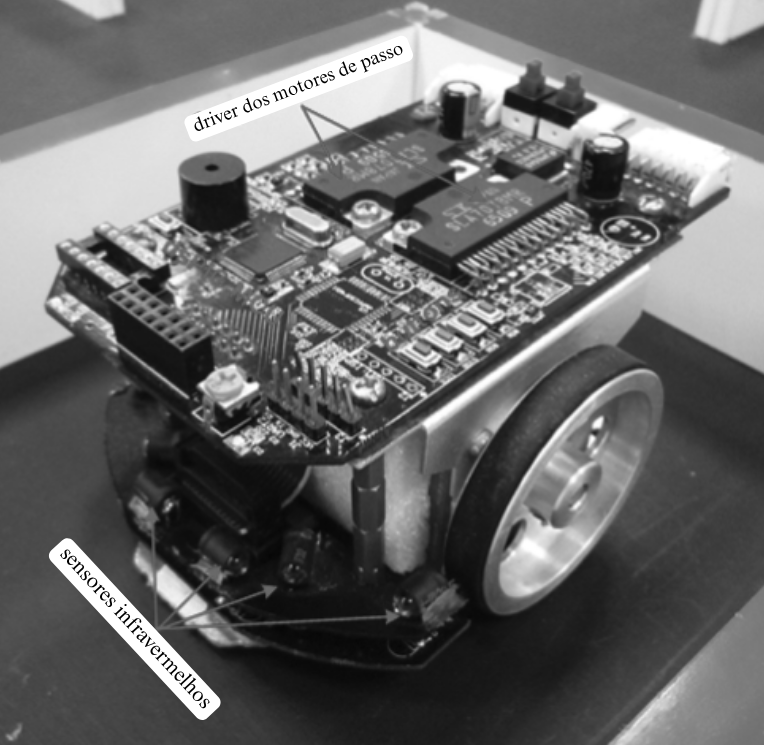
\includegraphics[width=7cm]{figuras/introducao/kit-micromouse-su-et-al.png}
        }{
            \Fonte{Adaptado de \citeonline{micromouse-kit-educational}}
        }	
    \end{figure}

    Em cenário nacional, é possível considerar ainda o trabalho de \citeonline{roberto-et-al-2024}, os quais desenvolvem um robô \textit{micromouse} desde o começo apresentando todos os seus aspectos construtivos e desenvolvendo as diversas malhas de controle para os cenários de resolução de labirinto. É cabível citar também o trabalho de \citeonline{dissetacao-pereira-2000}, o qual -- apesar de não abordar diretamente sobre resolução de labirintos -- desenvolve análises importantes dos aspectos cinemáticos, dinâmicos e dentro da teoria de controle, que podem ser aplicados para a implementação de robôs móveis e com restrições de movimento.

    \section{Motivação} \label{sec:motivacao}

        O desenvolvimento de um \textit{micromouse}, caracteriza-se por seu caráter multidisciplinar, uma vez que integra conhecimentos advindos de outras áreas da Engenharia. A concepção desse tipo de sistema demanda competências relacionadas ao desenvolvimento de eletrônica embarcada, técnicas de programação (muitas vezes envolvendo linguagens de alto e baixo nível simultaneamente), teoria de Controle, implementação de algoritmos inteligentes, projeto de placas de circuito impresso, modelagem mecânica do movimento, conhecimento de micromotores elétricos, integração de sensores, sistemas de comunicação sem fio, entre outras tecnologias essenciais para a operação autônoma do robô \cite{kim-byung-2020}.

        % Dos pontos enumerados anteriormente, alguns podem ser contornados total ou parcialmente com a adoção de modelos já prontos como, por exemplo, o kit educacional em \citeonline{micromouse-kit-educational} ou, para o caso do presente trabalho o kit desenvolvido em \citeonline{manual-microumouse-2015}.

        Parte desses desafios pode ser reduzida por meio da utilização de plataformas já consolidadas. Como exemplos, podem ser citados o kit educacional apresentado em \citeonline{micromouse-kit-educational} e, no contexto deste trabalho, a plataforma descrita em \citeonline{manual-microumouse-2015}, a qual serviu de base para o desenvolvimento realizado.

        % Entretanto, os tópicos relativos à programação, à modelagem e ao controle não são contornados dessa forma, haja vista que a forma com que são construídos, visando trabalhar em diferentes situações e ambientes, faz com que essas questões devam ser adaptadas a cada realidade.

        Entretanto, os aspectos relacionados à programação, à modelagem e ao controle do sistema permanecem fortemente dependentes da aplicação considerada. Embora modelos previamente desenvolvidos forneçam uma estrutura funcional para o robô, os algoritmos de controle e navegação devem ser adequadamente adaptados às características da plataforma utilizada e às condições específicas do ambiente de operação.

        % Portanto, neste cenário, este trabalho se motiva pelo estudo do controle aplicado ao robô \textit{micromouse} disponível no laboratório da \gls{UFPI} através do grupo \gls{GRASI}. Para isso é feita uma análise da cinemática/dinâmica do robô e do comportamento dos seus motores com sinais de excitação, especialmente para a resposta ao degrau unitário na presença de sinais \gls{PRBS}. Conjuntamente, são projetados controladores monovariáveis para atuar nas dinâmicas individuais dos motores e na dinâmica global do robô. Por fim, são desenvolvidos algorítmos \textit{seguidores de parede} os quais são a base para algumas das técnicas de resolução de labirintos. 

        Nesse contexto, este trabalho tem como motivação o estudo e o desenvolvimento de estratégias de controle aplicadas ao robô \textit{micromouse} disponível no Laboratório de Controle e Automação do curso de Engenharia Elétrica da \gls{UFPI}, por meio das atividades desenvolvidas no âmbito do grupo \gls{GRASI}. Para isso, é realizada uma análise da cinemática e da dinâmica do robô, bem como do comportamento dinâmico de seus motores diante de diferentes sinais de excitação, com ênfase na resposta ao degrau e na utilização de sinais \gls{PRBS} para fins de identificação e caracterização do sistema.

        De posse dos modelos obtidos, são projetados controladores monovariáveis destinados ao controle das dinâmicas individuais dos motores e das variáveis globais de movimento do robô. Adicionalmente, são desenvolvidos algoritmos do tipo \textit{seguidor de parede}, amplamente empregados em estratégias de navegação e considerados a base para diversos métodos clássicos de resolução de labirintos utilizados em competições de \textit{micromouse}.

    % objetivos
    \section{Objetivos} \label{sec:objetivos}

        \subsection{Objetivo Geral} \label{ssec:objetivo-geral}

        Desenvolver e implementar estratégias de controle de velocidade e telemetria para um robô autônomo do tipo \textit{micromouse}, visando melhorar seu desempenho de navegação e movimentação.

        \subsection{Objetivos Específicos} \label{ssec:objetivos-especificos}

        \begin{itemize}
            \item Identificar e modelar o comportamento dos motores através da descrição no tempo, \gls{FT} e equações a diferenças.
            \item Estudar o comportamento diferencial do robô \textit{micromouse} por meio de equações cinemáticas.
            \item Projetar, implementar e avaliar controladores básicos do tipo \gls{PID} para os motores e para as velocidades globais do robô, com o uso de malhas de controle e de supervisão.
            \item Desenvolver estratégias de comunicação sem fio que permitam a telemetria e a adequada coleta de informações do robô \textit{micromouse} mesmo quando não estiver fisicamente próximo ao \gls{PC}.
            \item Desenvolver algorítmos em linguagem de programação \textit{C} que possam ser aplicadas a sistemas embarcados a partir da adapatação de algoritmos desenvolvidos em linguagem \textit{MATLAB}.
        \end{itemize}

    % seções 
    \section{Organização do Trabalho} \label{sec:organização}

        O presente trabalho está dividido em cinco capítulos. No Capítulo \ref{cap:id-e-controle} são apresentadas as bases matemáticas e teóricas essenciais para o desenvolvimento da modelagem e do controle. Em seguida, no Capítulo \ref{cap:micromouse}, o robô \textit{micromouse} é melhor apresentado, bem como suas características construtivas, programação e também a análise da sua movimentação. Já no Capítulo \ref{cap:metodologia} está contida a metodologia desenvolvida desde o processo de estudo e preparação, passando pela aquisição e telemetria dos dados até a identificação e implementação do controle. O Capítulo \ref{cap:resultados}, por sua vez, apresenta os resultados obtidos na modelagem e nos testes de controle. Por fim, o Capítulo \ref{cap:conclusoes-e-trabalhos-futuros} apresenta as conclusões desta pesquisa bem como os trabalhos futuros sugeridos.


	

	

	% \chapter{Metodologia}
\label{cap:metodologia}

% Neste capítulo será apresentada a metodologia utilizada para o desenvolvimento do trabalho. Estruturada da seguinte maneira: na seção \ref{sec:preparacao}, serão apresentados os aspectos relacionados a preparo do robô para a realização de experimentos; na seção \ref{sec:coleta-dados} será abordada a questão de como realizar a coleta de dados para identificação e controle; na seção \ref{sec:id-controle-classico-metodologia}, será apresentada a abordagem utilizada para realização da identificação e controle do robô \textit{micromouse}.

A metodologia utilizada para o desenvolvimento do trabalho foi estruturada em quatro etapas. Inicialmente foram realizados estudos para a adequação do robô \textit{micromouse} disponível no Laboratório de Controle e Automação do \gls{GRASI} do curso de Engenharia Elétrica da \gls{UFPI}. Em seguida, foram realizados estudos e alterações ao nível de \textit{software} para o desenvolvimento da telemetria e do controle do robô. A etapa seguinte consistiu no desenvolvimento dos algoritmos de controle e de identificação para o robô \textit{micromouse}. Por fim, foram executados testes para avaliação das soluções adotadas.

    \section{Preparação inicial} \label{sec:preparacao}
    
        Para a execução de um percurso o mais próximo possível ao ideal, é necessário que o micromouse tenha seus componentes operando, também, o mais próximo da idealidade. Assim, são necessárias serem feitas manipulações mecânicas, e também de software, no robô. 
        
        \subsection{Manipulação mecânica} \label{ssec:manipulacao-mecanica}
            As alterações mecânicas, por sua vez, consistiram em trocar as rodas originais que se encontravam danificadas por rodas semelhantes, porém modeladas e impressas em 3D. A vantagem principal se dá pelo fato de ao possuir um modelo tridimensionald da roda é possível realizar novas impressões em caso de danos causados a estrutura original dessas, com um custo menor que em caso de substituição por peças originais. 
            
            As Figuras \ref{fig:modelo_roda_3d} e \ref{fig:roda_impressa_3d}, a seguir, apresentam, respectivamente, o modelo 3D das rodas originais e a novas impressas.

            \begin{figure}[htbp]
                \centering
                \begin{minipage}{0.45\textwidth}
                    \centering
                    \Caption{\label{fig:modelo_roda_3d} Modelo 3D}
                    %\centering
                    \UFCfig{}{
                        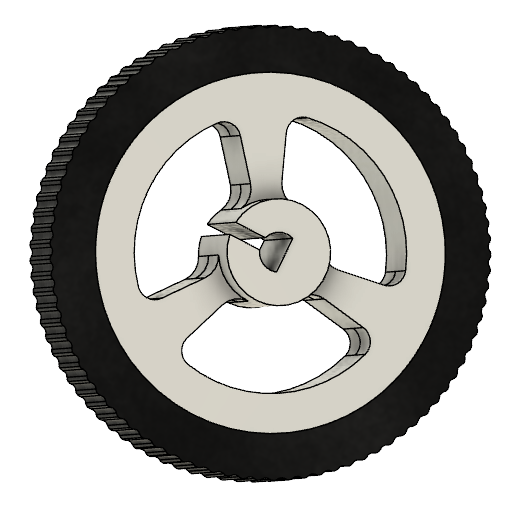
\includegraphics[width=4cm]{figuras/metodologia/modelo_3d_roda.png}
                    }{
                        \Fonte{O autor}
                    }	
                \end{minipage}
                \hfill
                \begin{minipage}{0.45\textwidth}
                    \centering
                    \Caption{\label{fig:roda_impressa_3d} Roda Impressa}
                    %\centering
                    \UFCfig{}{
                        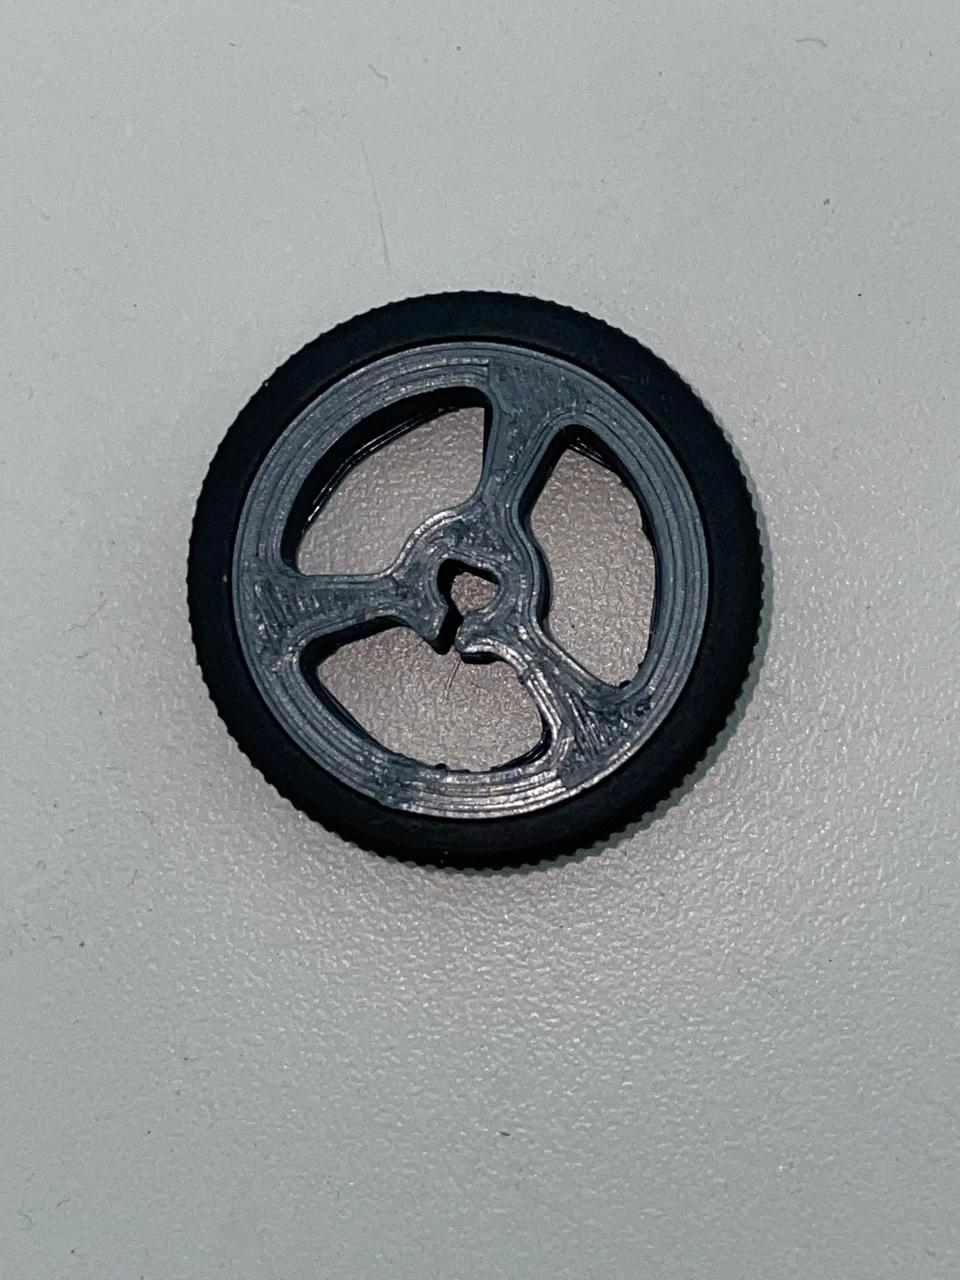
\includegraphics[width=4cm]{figuras/metodologia/roda_impressa.jpg}
                    }{
                        \Fonte{O autor}
                    }	
                \end{minipage}
            \end{figure}
        
        \subsection{Manipulação de software} \label{ssec:manipulacao-sowftware}
            As alterações via software correspondem à programação desenvolvida e embarcada no microcontrolador. No presente trabalho pode-se destacar 3 ferramentas de produção de código utilizadas. São elas as seguintes \gls{IDE} (sigla em inglês para Ambiente de Desenvolvimento Integrado): \gls{VSCode}, MATLAB e Eclipse IDE.

            O \gls{VSCode}, é um editor de códigos desenvolvido pela \textit{Microsoft} que pode ser utilizado com diferentes linguagens de programação, entre elas linguagens C e C++, as quais foram usadas para programar os microcontroladores ESP32 e ESP8266, abordada em \ref{ssec:comunicacao}.

            O MATLAB, por sua vez, é uma \gls{IDE} e uma linguagem de programação com foco em computação numérica e análise de dados \cite{matlab-def}. Esse ambiente foi utilizado para recebimento dos dados e para desenvolvimento dos algorítmos de identificação bem como para obtenção dos parâmetros dos controladores posteriormente embarcados no robô.

            Por fim, o Eclipse IDE foi usado na sua versão para sistemas embarcados (\textit{for Embedded  C/C++ Developers}) para produção dos códigos que a serem embarcados no \textit{micromouse}. Esta versão, conforme \citeonline{eclipse-def}, possui plug-ins de compilação cruzada (\textit{cross build}) e de suporte a arquiteturas ARM e RISC-V.

            % A seguir são apresentadas, nas figuras \ref{fig:vscode-interface}, \ref{fig:matlab-interface} e \ref{fig:eclipse-interface}, respectivamente, as interfaces do \gls{VSCode}, do MATLAB e do Eclipse IDE.


            % \begin{figure}[htbp]
            %     \centering
            %     \Caption{\label{fig:vscode-interface} Interface do \gls{VSCode}}	
            %     \UFCfig{}{
            %         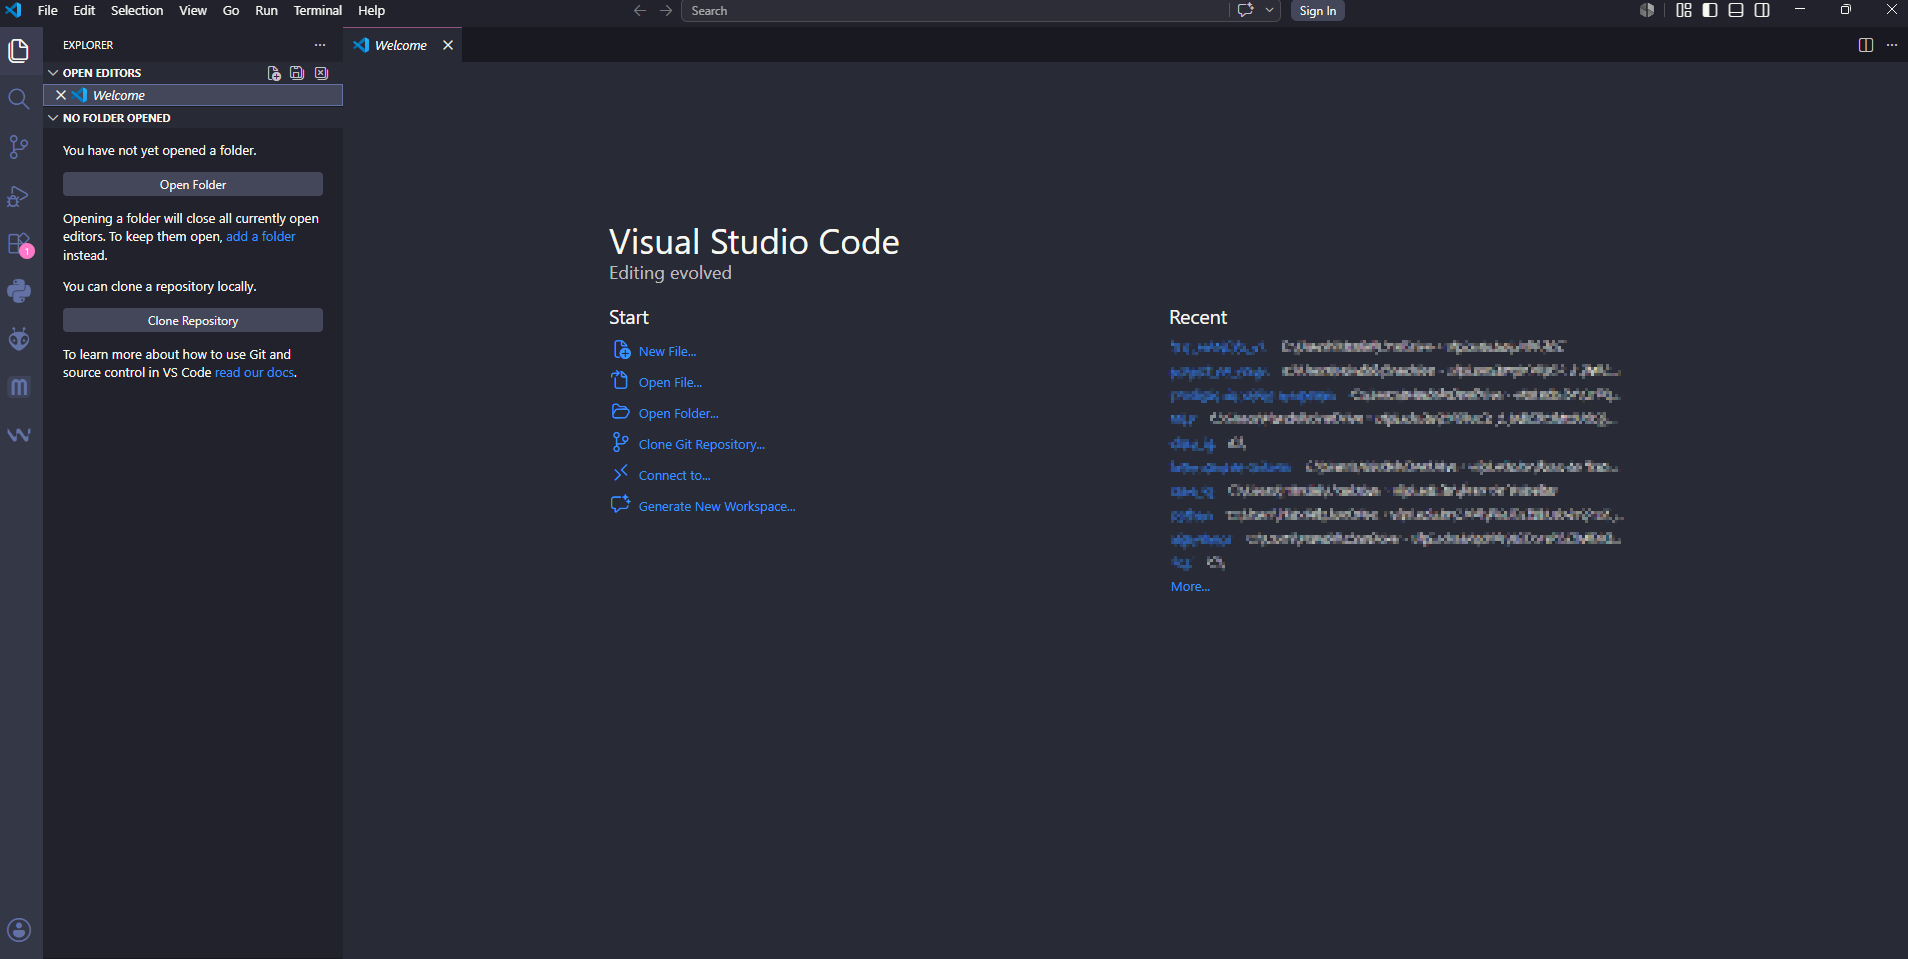
\includegraphics[width=8cm]{figuras/metodologia/interface_vscode.png}
            %     }{
            %         \Fonte{O autor}
            %     }	
            % \end{figure}

            % \begin{figure}[htbp]
            %     \centering
            %     \Caption{\label{fig:matlab-interface} Interface do MATLAB}	
            %     \UFCfig{}{
            %         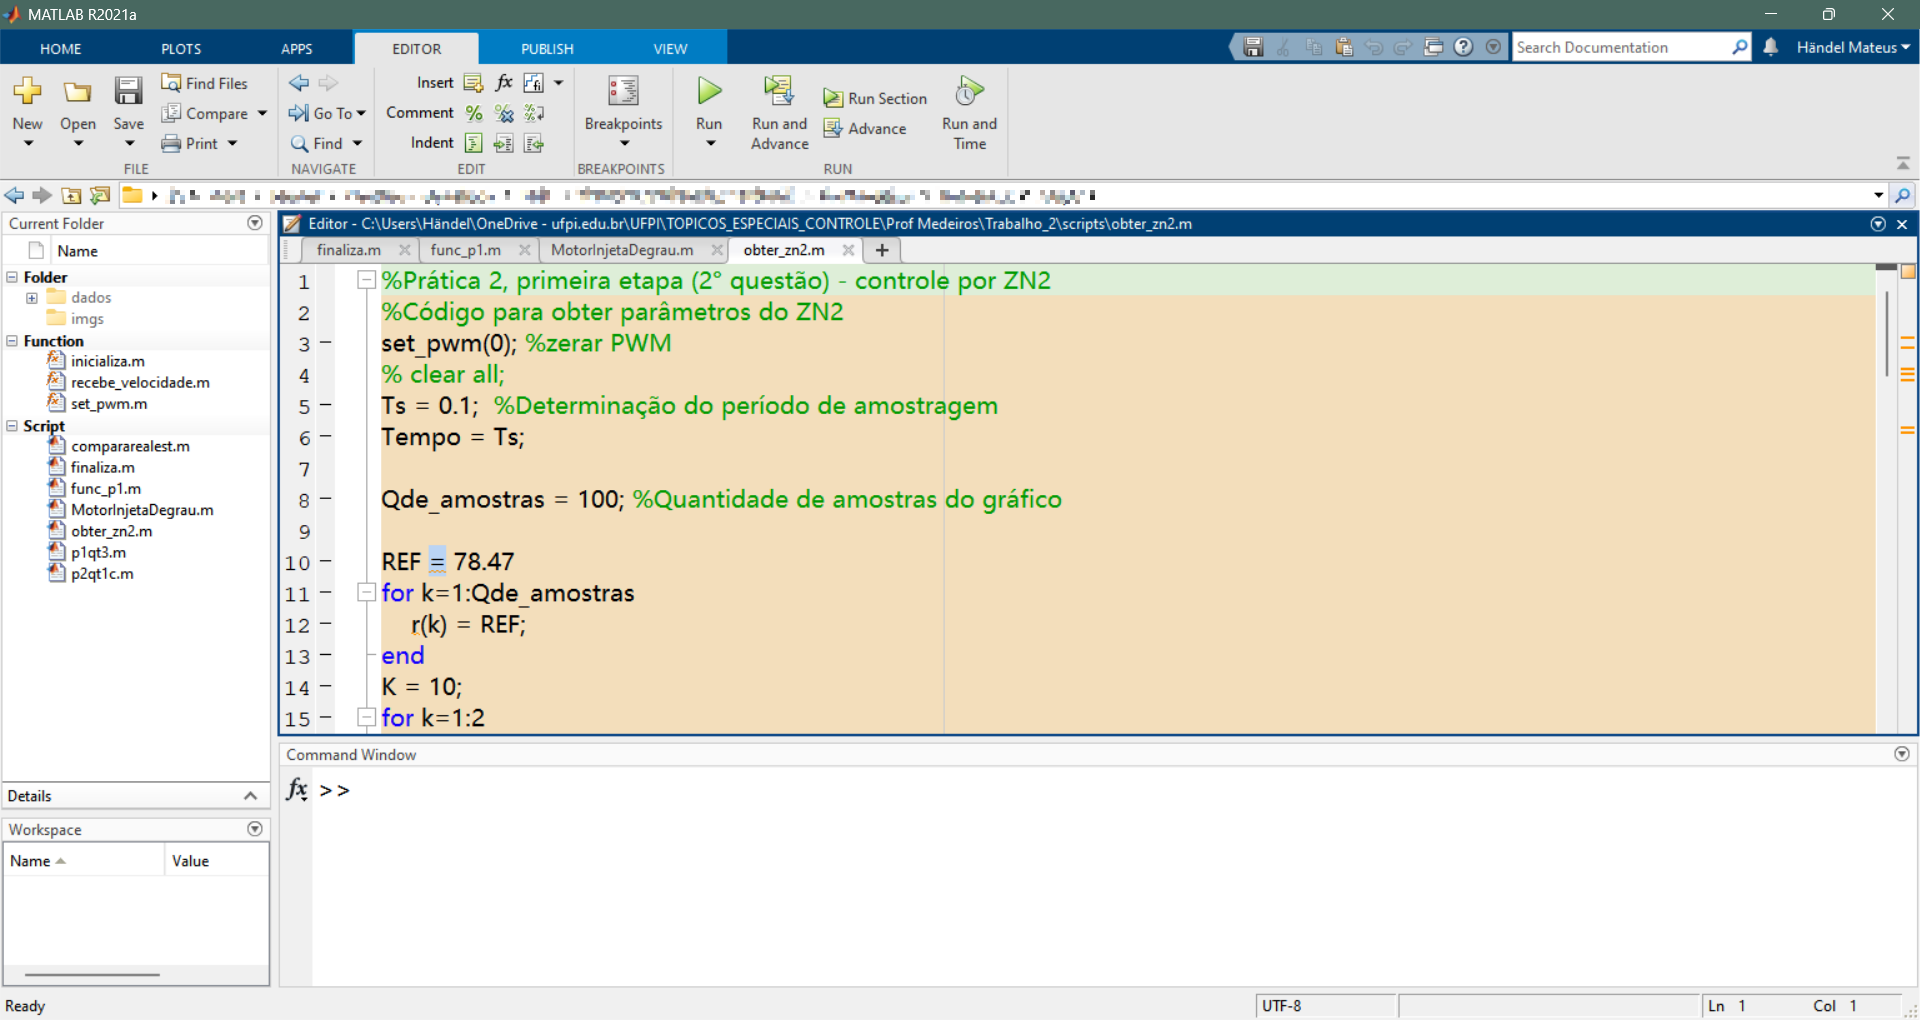
\includegraphics[width=8cm]{figuras/metodologia/interface_matlab.png}
            %     }{
            %         \Fonte{O autor}
            %     }	
            % \end{figure}

            % \begin{figure}[htbp]
            %     \centering
            %     \Caption{\label{fig:eclipse-interface} Interface do Eclipse IDE}	
            %     \UFCfig{}{
            %         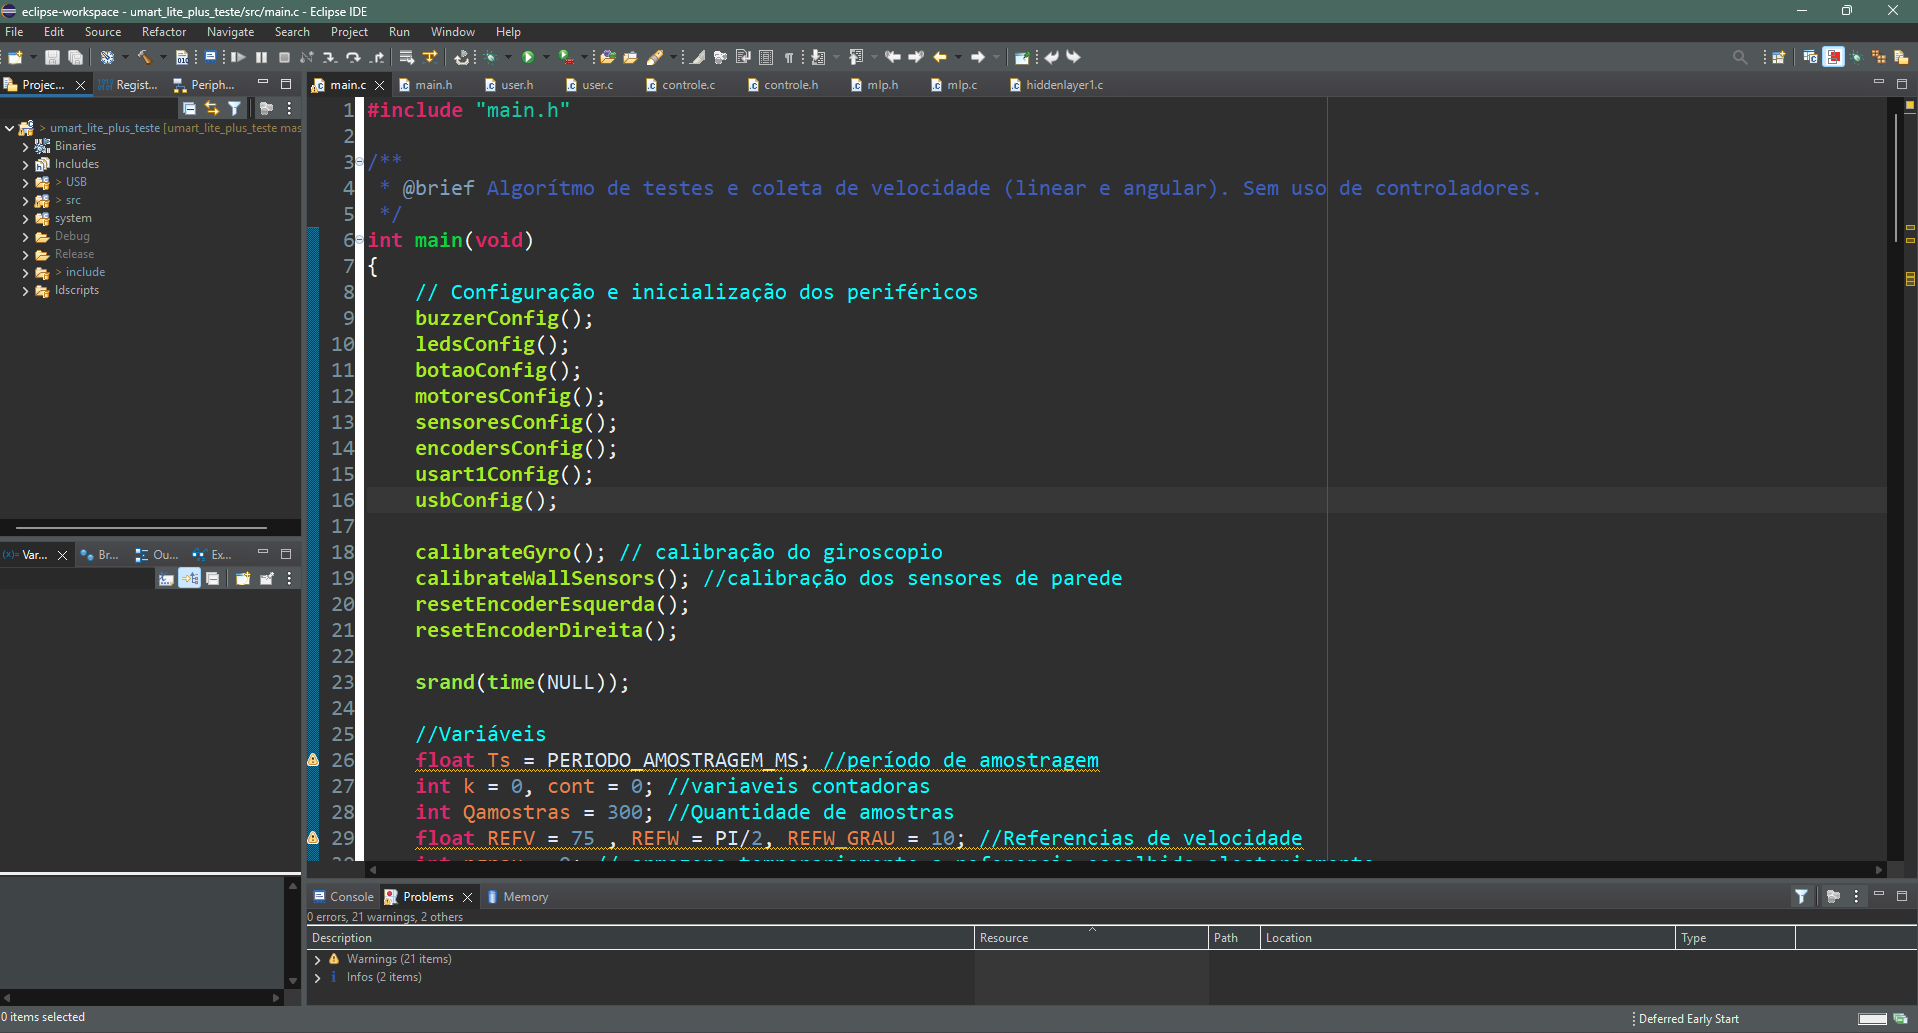
\includegraphics[width=8cm]{figuras/metodologia/interface_eclipse.png}
            %     }{
            %         \Fonte{O autor}
            %     }	
            % \end{figure}
    
    \section{Coleta de Dados} \label{sec:coleta-dados}
        Um passo necessário para realização de todo o processo de controle e monitoramento do comportamento do robô é a transferência das informações coletadas localmente para o computador. Em plantas fixas muitas vezes essa comunicação é realizada via cabo com comunicação serial, dada a sua praticidade de implementação e velocidade de transmissão. Entretanto, devido à natureza móvel da planta do presente trabalho, a necessidade muda e passa a ser a de uma comunicação que, ao menos em parte, seja sem fio. 
        
        Contudo, conforme visto em \ref{sec:caracteristicas-construtivas} o robô não dispõe de instrumentos de comunicação sem fio nativas. Por isso, inspirado no trabalho desenvolvido por \citeonline{tcc-artemio}, foi elaborada uma arquitetura de rede local de comunicação e telemetria que faz uso de dois microcontroladores do tipo ESP que trocam informações entre si via WiFi, através do protocolo ESP-NOW, sendo um do modelo ESP8266 e um ESP-WROOM-32. O ESP8266 foi escolhido devido a seu tamnho reduzido o que facilita a construção de uma estrutura para conectá-lo ao robô. O ESP-WRROM-32 foi utilizado em virtude da sua disponibilidade em laboratório. 
        
        O modelo ESP8266 está conectado ao robô e o ESP-WROOM-32 a um computador de tal modo que após a execução de um experimento a comunicação é ativada e, via serial os dados são enviados do robô para o ESP8266 e estes são transmitidos então para o ESP-WROOM-32, o qual as envia para o \gls{PC}. 
        
        As figuras \ref{fig:esp-wroom-32} e \ref{fig:esp-8266} mostram os dois microcontroladores ESP utilizados e a Figura \ref{fig:rede-comunicacao} ilustra a arquitetura descrita acima. Nesta figura o robõ encontra-se representado pelo \textit{microchip} STM32F405RGT6 apresentado à esquerda, ilustrando o seu centro de processamento dos dados.

        \begin{figure}[htbp]
            \centering
            \begin{minipage}{0.45\textwidth}
                \centering
                \Caption{\label{fig:esp-wroom-32} ESP-WROOM-32}
                %\centering
                \UFCfig{}{
                    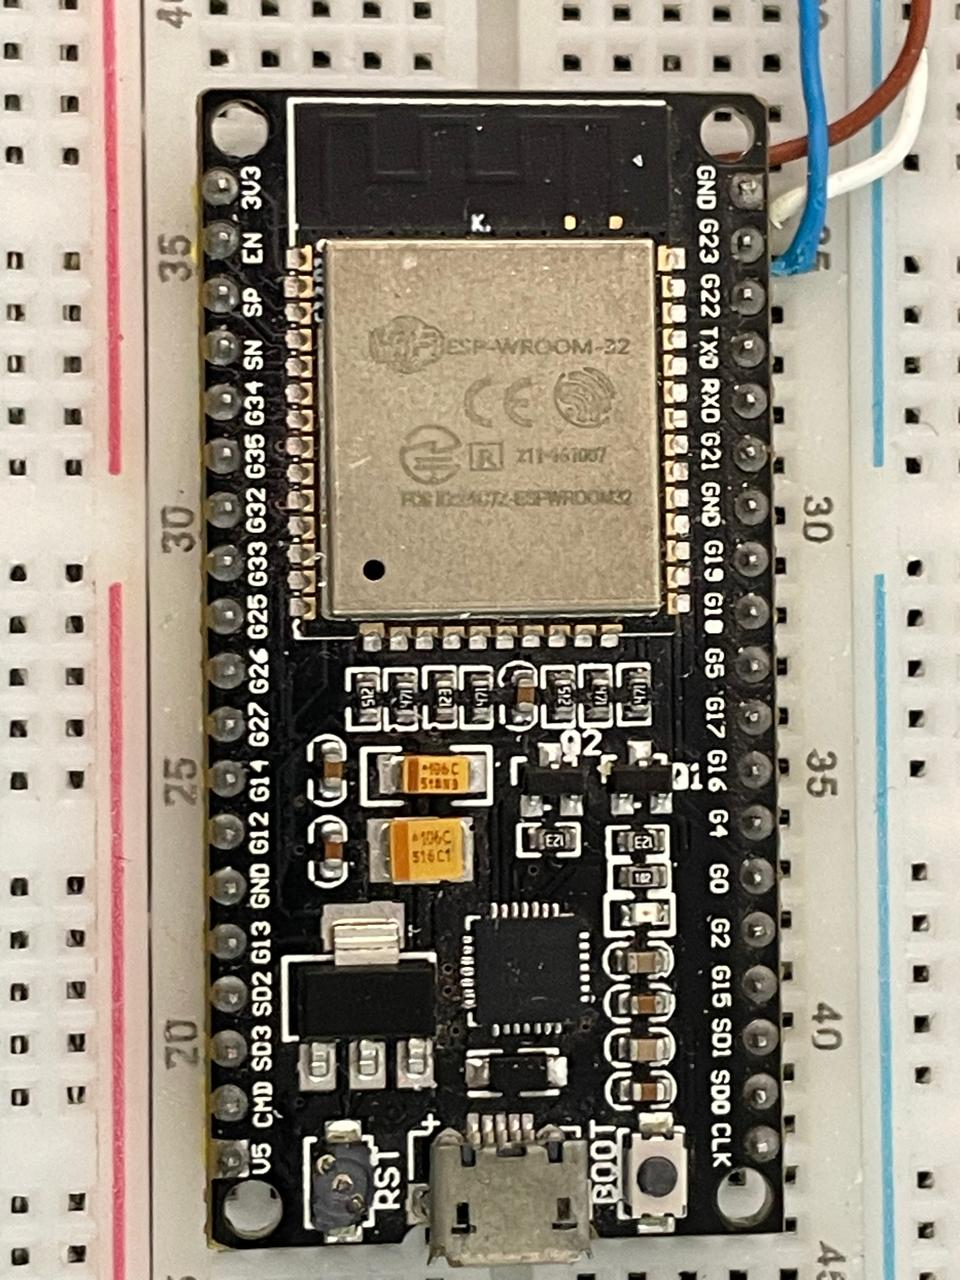
\includegraphics[width=3cm]{figuras/metodologia/esp32-wroom-32.jpg}
                }{
                    \Fonte{O autor}
                }	
            \end{minipage}
            \hfill
            \begin{minipage}{0.45\textwidth}
                \centering
                \Caption{\label{fig:esp-8266} ESP8266}
                %\centering
                \UFCfig{}{
                    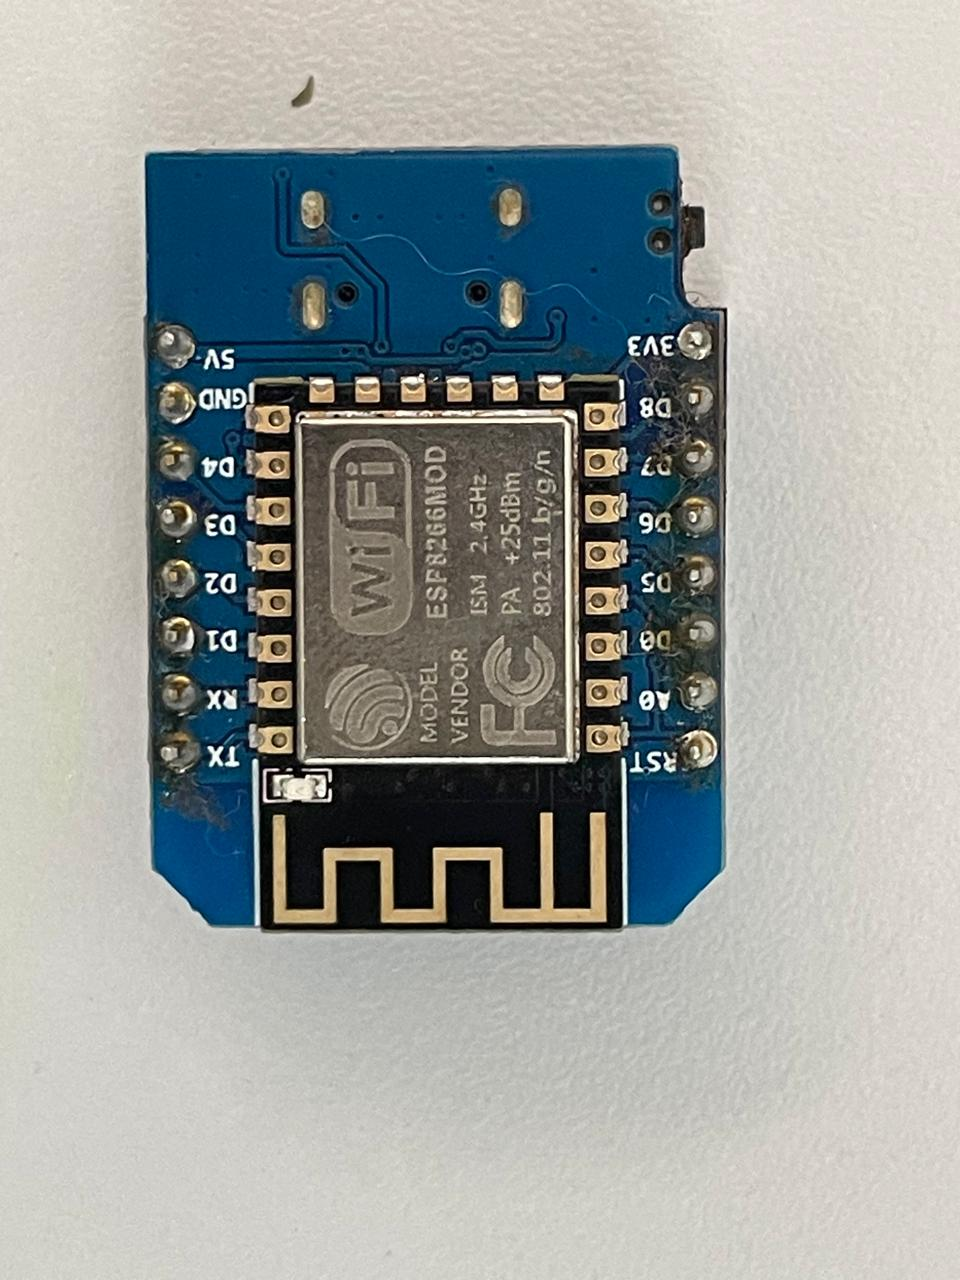
\includegraphics[width=3cm]{figuras/metodologia/esp8266-d1mini.jpg}
                }{
                    \Fonte{O autor}
                }	
            \end{minipage}
        \end{figure}

        \begin{figure}[htbp]
                \centering
                \Caption{\label{fig:rede-comunicacao} Arquitetura de rede de comunicação desenvolvida para envio de informações}	
                \UFCfig{}{
                    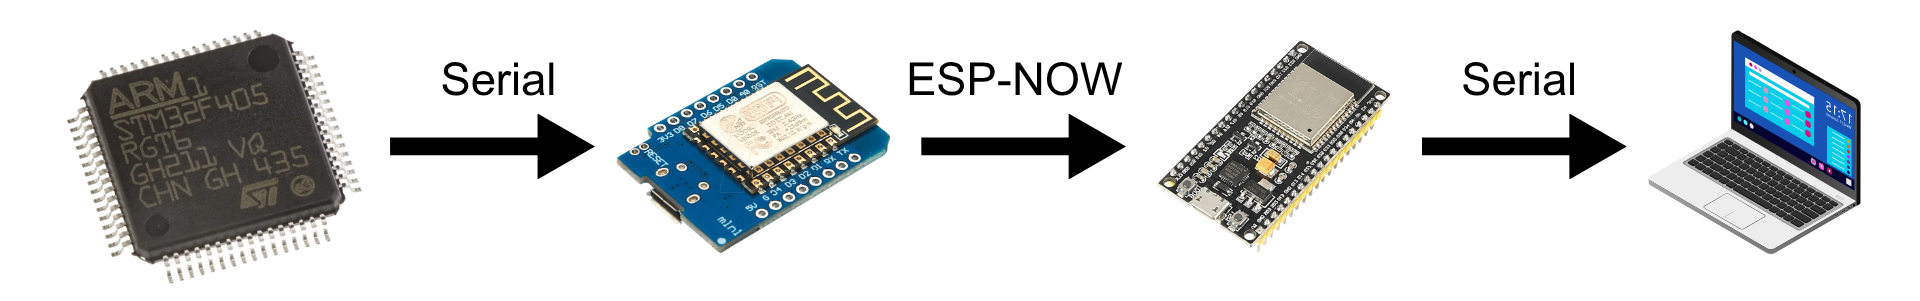
\includegraphics[width=12cm]{figuras/metodologia/rede-comunicacao-cropped.png}
                }{
                    \Fonte{O autor}
                }	
        \end{figure}

        \subsection{Comunicação e Telemetria} \label{ssec:comunicacao}
            A estrutura apresentada na Figura \ref{fig:rede-comunicacao} pode ainda ser interpretada como sendo composta por dois grupos que trocam informações via WiFi. O primeiro grupo está composto pelo STM32F405RGT6 e pelo ESP8266 e fica localizado no espaço físico do robô, onde o primeiro chip está soldado à placa e o segundo está conectado através da entrada do conector \textbf{J2} (\gls{UART}), conforme descrito em \citeonline{manual-microumouse-2015} e mostrado na Figura \ref{fig:micromouse-composicao} (aparece como “conector para módulo bluetooth”). O segundo grupo, por sua vez, é formado pelo ESP-WROOM-32 e pelo \gls{PC}, está localizado separado do robô, na bancada de trabalho, utilizando um cabo \gls{USB} para comunicação.

            \subsubsection{Comunicação Serial} \label{sssec:comunicacao-serial}
                Para a realização da comunicação no primeiro grupo foi optada pelo protocolo \gls{UART}. Nesse protocolo faz-se necessário que ambos os dispositivos possuam a mesma taxa de transferência de dados (\textit{baud rate}), haja vista a ausência de um sinal \gls{CLK} para orientar o tempo de envio dos bits. No presente trabalho foi feita a opção pela taxa de 9600 \textit{bps}, que foi a taxa que também foi adotada para o grupo contendo o ESP-WROOM-32 e o \gls{PC}.

                Para a comunicação entre o ESP-WROOM-32 e o \gls{PC} foi utilizado um cabo \gls{USB} como meio físico. Já para a comunicação entre o STM32F405RGT6 e o ESP8266 desenvolveu-se uma \gls{PCI} para ser integrada ao conector \textbf{J2} do \textit{micromouse} para realizar a conexão dos pinos de \textbf{3V3}, \textbf{GND}, \textbf{RX}, e \textbf{TX} conforme a imagem abaixo.

                \begin{figure}[htbp]
                    \centering
                    \Caption{\label{fig:conexao-stm-esp8266} Conexão de pinos entre o STM32F405RGT6 e o ESP8266}	
                    \UFCfig{}{
                        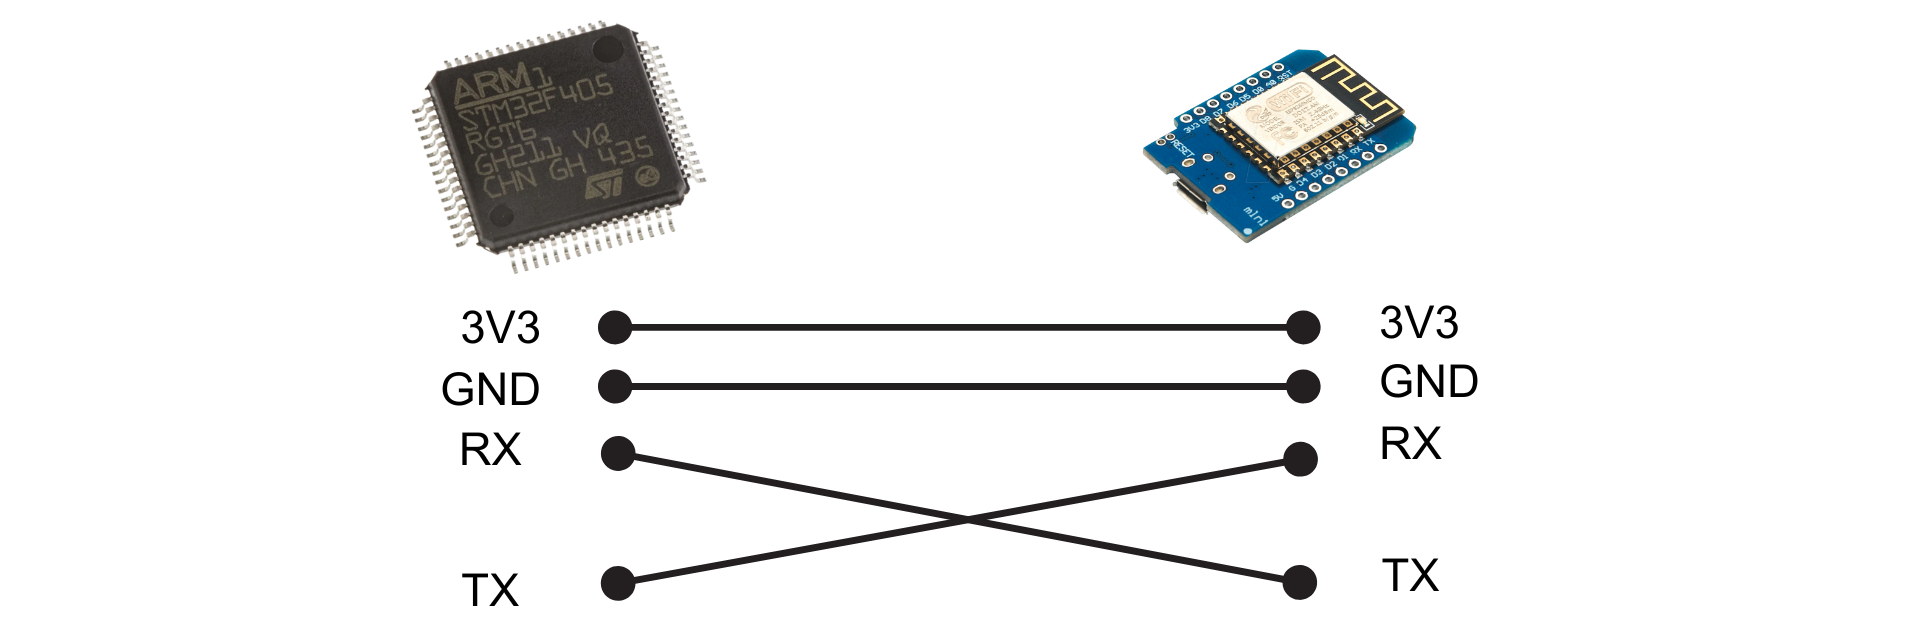
\includegraphics[width=12cm]{figuras/metodologia/uart-stm-esp8266-cropped.png}
                    }{
                        \Fonte{O autor}
                    }	
                \end{figure}

                A \gls{PCI} pode ser visualizada abaixo em seu esquemático na Figura \ref{fig:esquematico-pci} e após a sua finalização na Figura \ref{fig:pci-feita}.

                \begin{figure}[htbp]
                    \centering
                    \begin{minipage}{0.45\textwidth}
                        \centering
                        \Caption{\label{fig:esquematico-pci} Esquemático da \gls{PCI}}
                        %\centering
                        \UFCfig{}{
                            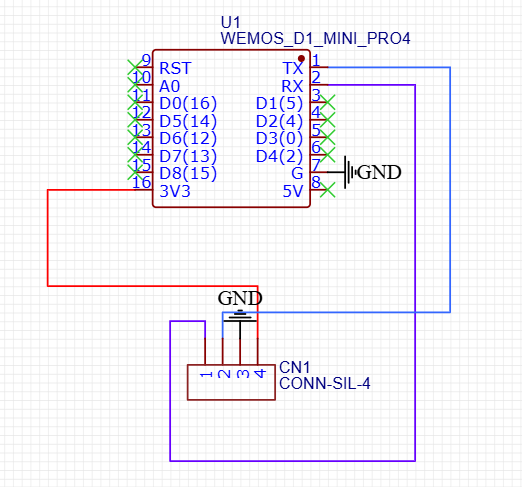
\includegraphics[width=4cm]{figuras/metodologia/esquematico_placa.png}
                        }{
                            \Fonte{O autor}
                        }	
                    \end{minipage}
                    \hfill
                    \begin{minipage}{0.45\textwidth}
                        \centering
                        \Caption{\label{fig:pci-feita} \gls{PCI} finalizada}
                        %\centering
                        \UFCfig{}{
                            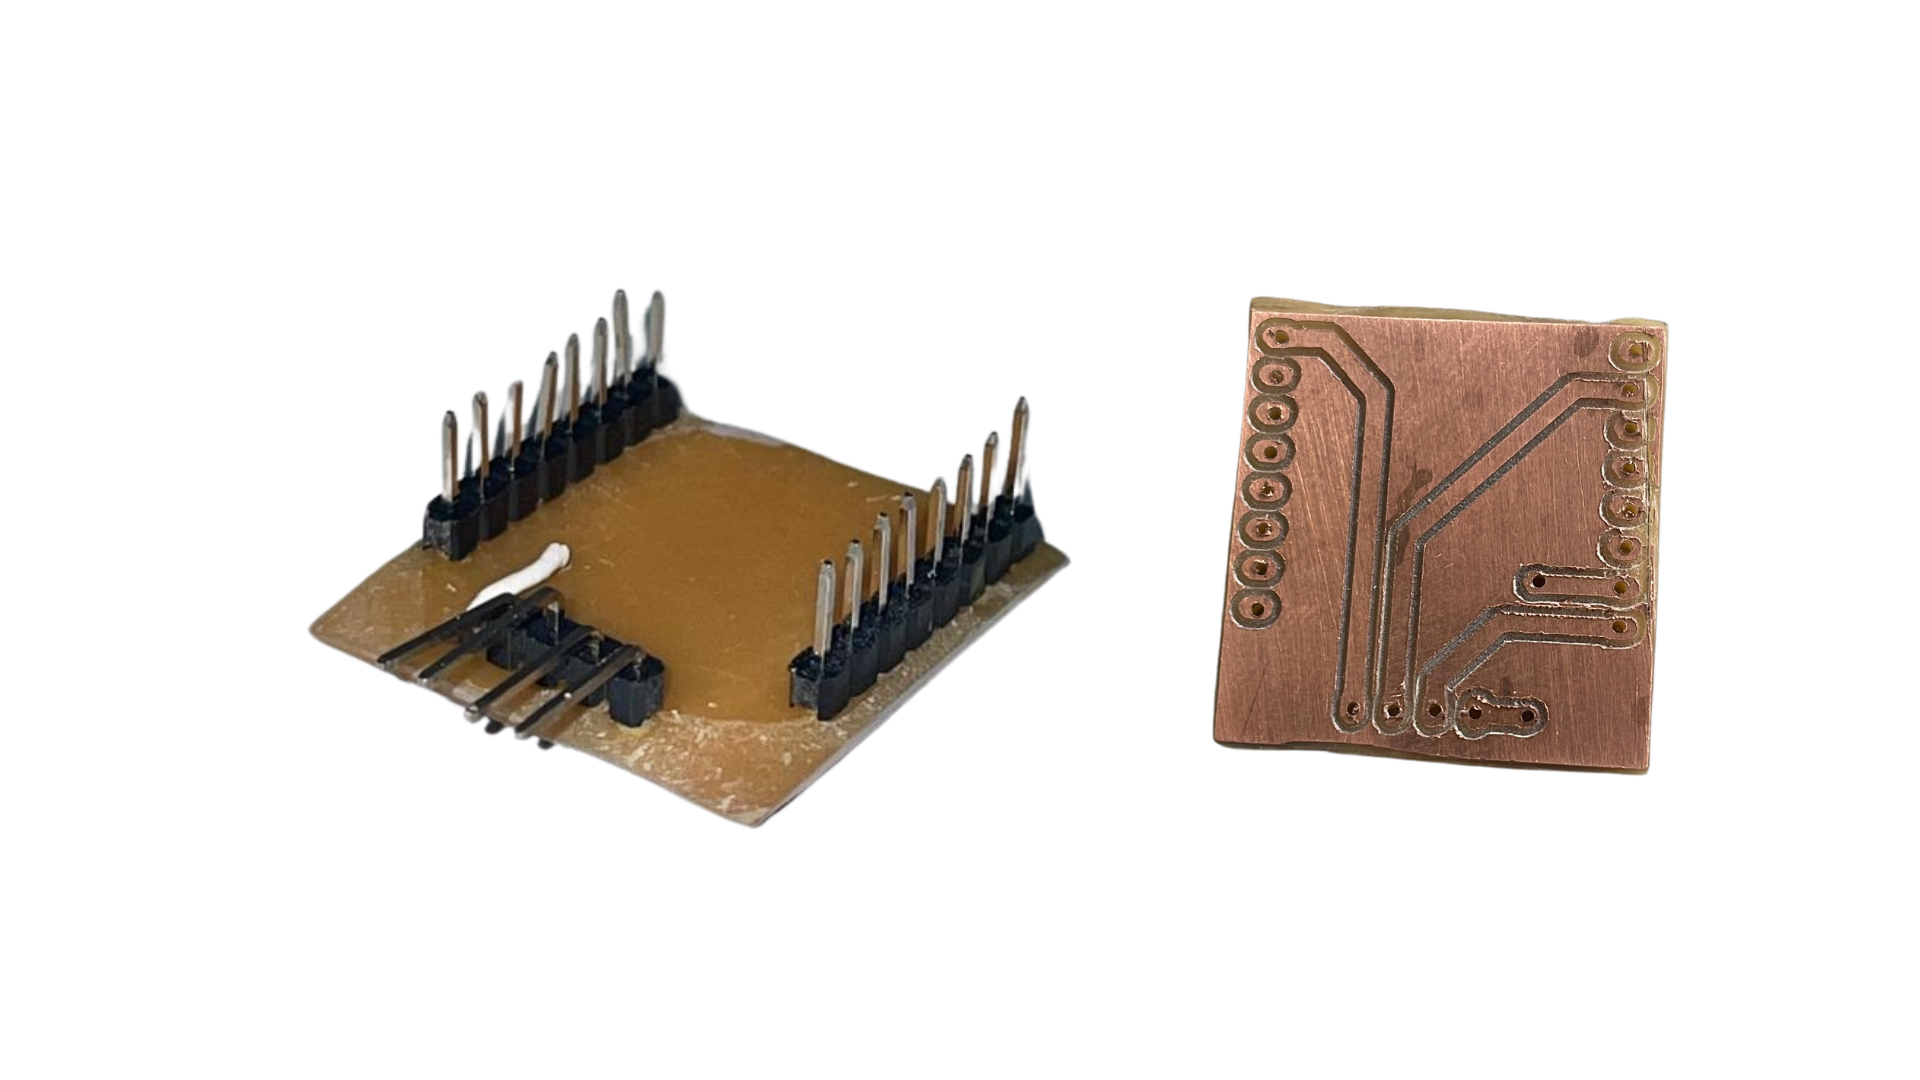
\includegraphics[width=4cm]{figuras/metodologia/placa_feita_cobre.png}
                        }{
                            \Fonte{O autor}
                        }	
                    \end{minipage}
                \end{figure}

            \subsubsection{Comunicação ESP-NOW} \label{sssec:comunicacao-esp-now}
                Conforme dito anteriormente, a comunicação sem fio se faz necessária pela natureza móvel da planta de estudo, o robô micromouse. O protocolo, desenvolvido pela \citeauthoronline{esp-now-definition},

                \begin{citacao}
                    \dots é um protocolo de comunicação sem fio baseado na camada de enlace de dados, que reduz as cinco camadas do modelo OSI para apenas uma. Assim, os dados não precisam ser transmitidos pelas camada de rede, de transporte, de sessão, de apresentação e de aplicação. Além disso, não há necessidade de cabeçalhos de pacote ou desempacotadores em cada camada, o que leva a uma resposta rápida, reduzindo o atraso causado pela perda de pacotes em redes congestionadas \cite[tradução do autor]{esp-now-definition}.
                \end{citacao}
                
                Dessa forma, o protocolo ESP-NOW se torna adequado para as necessidades de execução do projeto. Isto fica ainda mais evidenciado a partir do trabalho desenvolvido por \citeonline{tcc-artemio} o qual realizou a comparação com outros protocolos de comunicação sem fio e evidenciou a vantagem da utilização do protocolo ESP-NOW.

                No presente trabalho os dois microcontroladores ESP foram configurados tanto para enviar quanto para receber dados. Para isso, em cada um deles foi configurado da seguinte forma: 
                
                \begin{alineas}
                    \item \textit{Wifi} no modo \textbf{\textit{Wifi Station}};
                    \item Gravação do endereço MAC de destino em cada dispositivo correspondente;
                    \item Configuração \textit{Master-Slave}:
                    \begin{subalineas}
                        \item ESP8266 como \textbf{\textit{Slave}};
                        \item ESP-WROOM-32 como \textbf{\textit{Master}}.
                    \end{subalineas}
                \end{alineas}

                Essa configuração implica que apesar dos dois dispositivos poderem realizar tanto o envio quanto o recebimento de dados a comunicação é coordenada pelo ESP conectado ao \gls{PC}.  

    \section{Identificação e Controle} \label{sec:id-controle-classico-metodologia}

        De posse da estrutura desenvolvida, prosseguiu-se para a etapa de aplicações experimentais, na qual são implementados e avaliados os controladores projetados para o robô \textit{micromouse}. Essa etapa contempla os processos de \textit{Identificação} e \textit{Controle}, as quais ocorreram tanto ao nível individual -- para cada um dos motores -- quanto o nível global -- da trajetória. 
        
        Os experimentos realizados envolvem a coleta de dados e a comparação das variáveis associadas ao movimento global do robô, permitindo verificar o comportamento do sistema em condições reais de operação. Dessa forma, os experimentos realizados possibilitam analisar a resposta dos motores aos sinais de controle e avaliar o desempenho das malhas implementadas na sua capacidade de manter o robô dentro das condições de referência.

        \subsection{Identificação e Controle dos motores} \label{ssec:controle-motores}
            
            A \textit{Identificação} pode ser subdividida nas seguintes etapas. 
            
            \begin{enumerate}
                \item Coleta de dados: Medição da velocidade dos motores.
                \item Transmissão: Transferência das informações coletadas.
                \item Identificação: Aplicação de algoritmo no software MATLAB.
            \end{enumerate}
            
            O item $1$ ocorre de maneira embarcada e é coordenada pelo microcontrolador STM32F405RGT6. Já o item $2$, por sua vez, ocorre pela ação conjunta de todos os componentes da rede de comunicação. Por fim, o item $3$ é realizado utilizando apenas o \gls{PC}.

            A medição precisa da velocidade dos motores constitui a etapa fundamental para a correta identificação do sistema, uma vez que a qualidade dos modelos obtidos depende diretamente da confiabilidade dos dados experimentais coletados. Erros nessa medição comprometem a estimação dos parâmetros do modelo e, consequentemente, o desempenho das estratégias de controle projetadas a partir dele.

            Dessa forma, tomando como base as funcionalidades já disponíveis na plataforma do \textit{micromouse}, foram desenvolvidas e adaptadas rotinas computacionais destinadas à aquisição e ao processamento dos sinais provenientes dos sensores de velocidade dos motores, as quais possibilitam a obtenção das variáveis necessárias para a caracterização dinâmica do sistema e para as etapas subsequentes de identificação e projeto de controladores. 

            Após a implementação das rotinas de medição, realizou-se a normalização dos sinais de entrada e saída dos motores, mapeando-os para o intervalo entre $0\%$ e $100\%$ a fim de padronizar a escala das variáveis manipuladas e medidas, facilitando a análise dos dados experimentais, a identificação dos modelos e o projeto dos controladores. 
            
            A utilização de variáveis normalizadas contribui para a uniformização das grandezas envolvidas nas etapas de controle em \gls{MA} e \gls{MF}, reduzindo problemas decorrentes de diferenças de escala entre sinais e simplificando a interpretação dos resultados obtidos.
        
            Na fase de comunicação, o STM32F405RGT6 envia dados ao ESP8266 via \gls{UART}, que os repassa ao ESP-WROOM-32, armazenando-os em estruturas separadas para cada motor. Posteriormente, os dados são transferidos ao \gls{PC} via \gls{USB}, onde o MATLAB solicita informações sobre o tipo de dado e o motor ao qual ele se refere. Assim, com os dados coletados, é possível analisar a resposta do sistema a diferentes entradas, como degrau, rampa ou sinais randomizados.
        
            Baseado em \citeonline{tcc-marcolino} e usando como resposta a entrada a um degrau, para determinação do período de amostragem dos motores, foi determinado um período de amostragem de $T_s = 10ms$. Além disso, aplicou-se então uma entrada randomizada em torno de um degrau de referência, oscilando entre $\pm 10\%$ desse mesmo degrau, e coletou-se a saída para cada um dos motores. A partir dos dados coletados é possível, então, aplicar o algoritmo do estimador \gls{MQNR} e, assim, prosseguir com a identificação e com o desenvolvimento dos controladores.
            
            O projeto dos controladores foi realizado segundo a autossintonia baseada no Método do Relé, descrita na Seção \ref{sec:autossintonia-rele}. Inicialmente, foram implementados controladores \gls{PID} para o controle individual da velocidade de cada roda do robô, conforme ilustrado na Figura \ref{fig:controle-motores-individuais}. Essa abordagem permite atuar diretamente sobre a dinâmica de cada motor, proporcionando melhor rastreamento de referência e reduzindo os efeitos de diferenças entre ambos os motores.

            \begin{figure}[htb]
                \centering
                \Caption{\label{fig:controle-motores-individuais} Controle dos Motores Individuais}	
                    \UFCfig{}{
                        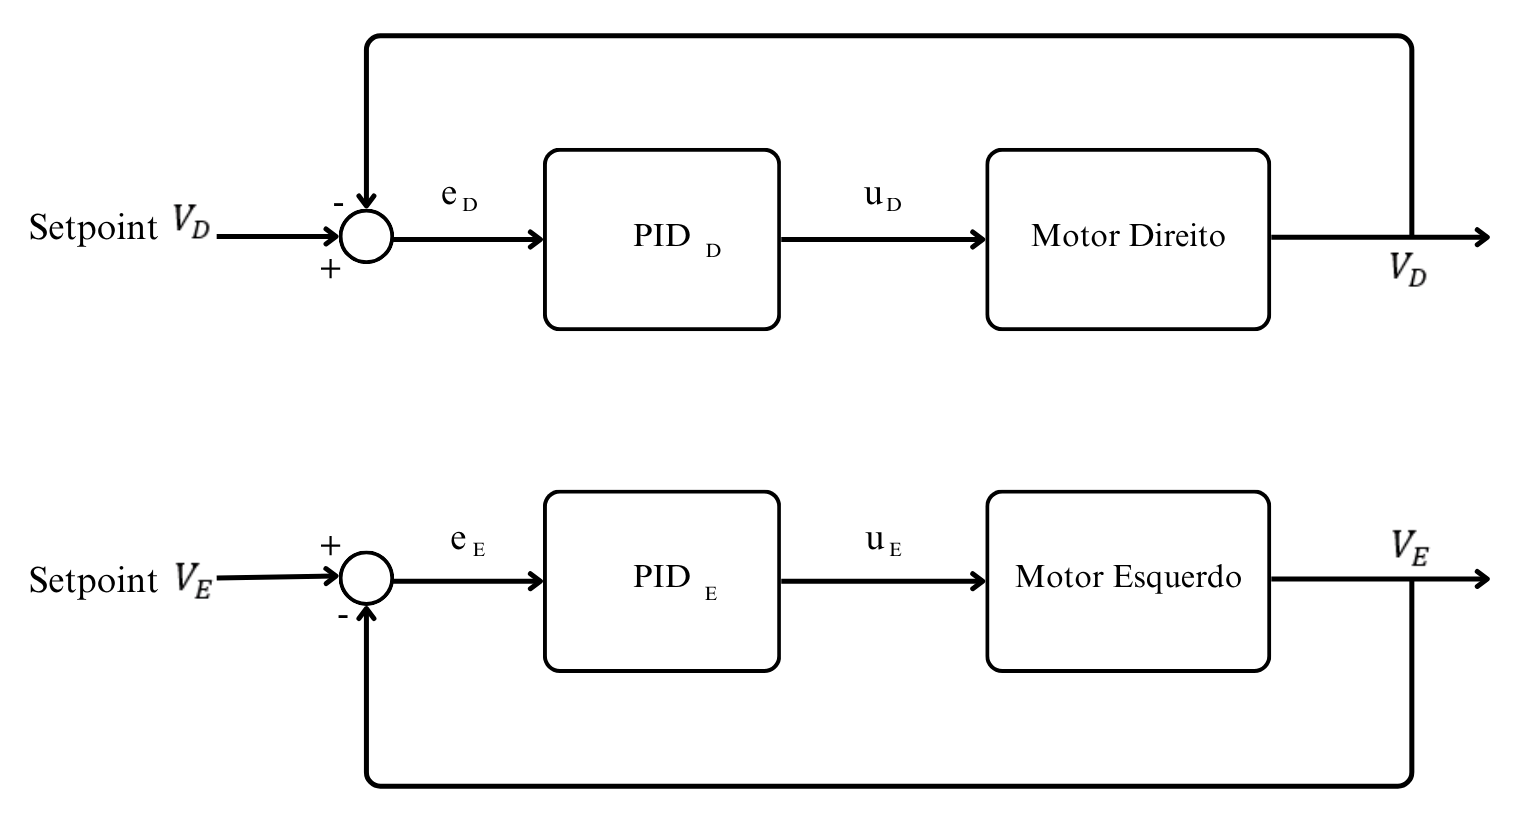
\includegraphics[width=9cm]{figuras/metodologia/malha-controle-motor-individual.png}
                    }{
                        \Fonte{O autor}
                    }	
            \end{figure}

        \subsection{Identificação e Controle das variáveis globais} \label{ssec:controle-trajetoria}

            Com os controladores individuais aplicados procedeu-se com a identificação e controle das variáveis globais de movimento do \textit{micromouse}, responsáveis pelo adequado seguimento de trajetória. A \textit{Identificação} seguiu os mesmos procedimentos apresentados anteriormente. Após isso, foram implementadas as duas malhas de controle de nível superior, denominadas como malhas \textit{supervisórias}, responsáveis pela geração dos \textit{setpoints} aplicados aos controladores individuais. 
            
            Conforme a Figura \ref{fig:controle-malhas-globais}, essas malhas atuam sobre as variáveis globais de movimento do robô, coordenando a ação dos controladores das rodas de modo a controlar o comportamento cinemático do \textit{micromouse} de forma integrada.        

            \begin{figure}[htb]
                \centering
                \Caption{\label{fig:controle-malhas-globais} Controle Supervisório Incluso}	
                    \UFCfig{}{
                        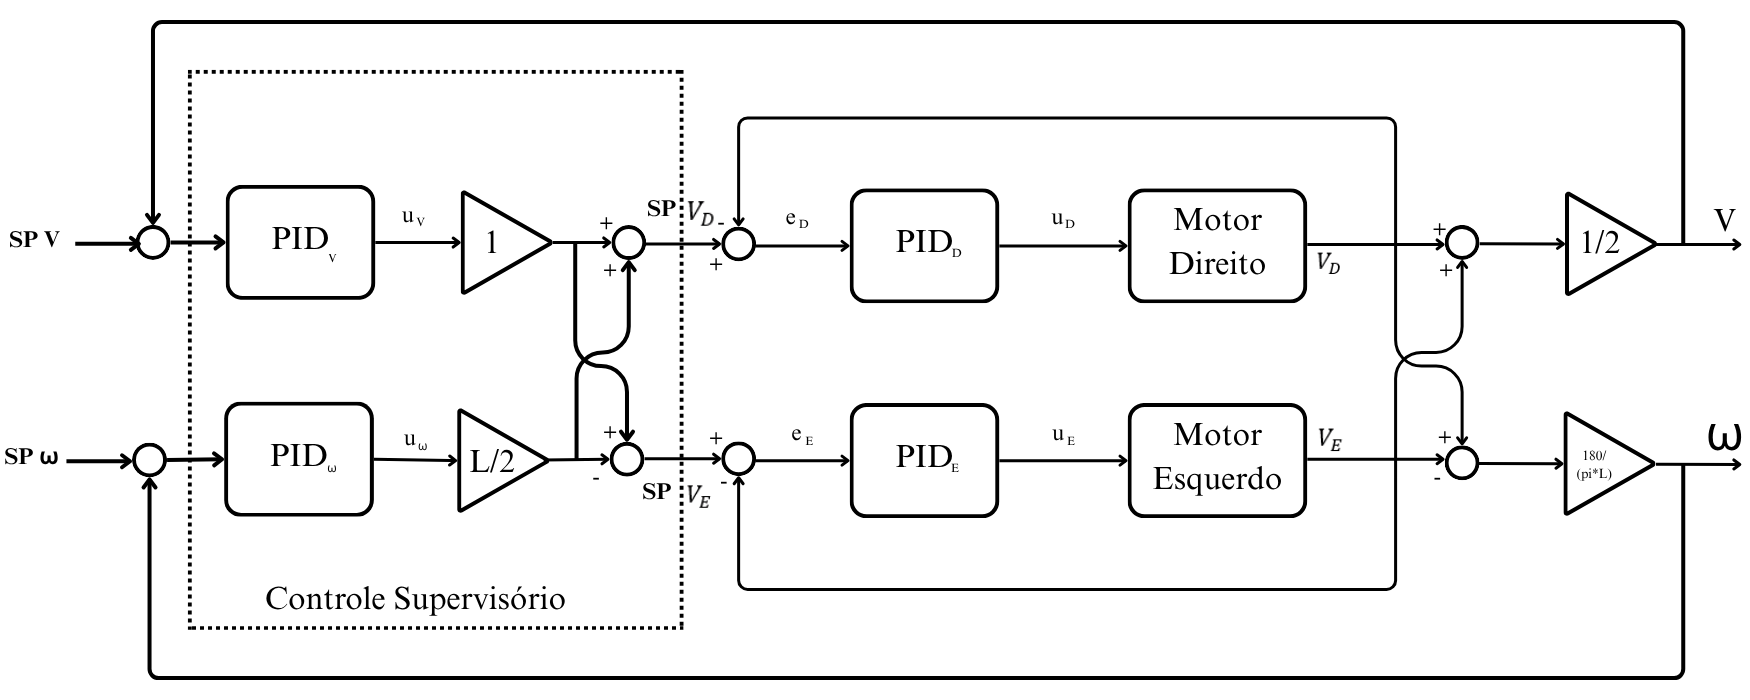
\includegraphics[width=16cm]{figuras/metodologia/malha-controle-global.png}
                    }{
                        \Fonte{O autor}
                    }	
            \end{figure}
            
            A partir da Figura \ref{fig:controle-malhas-globais} observa-se, também, a inclusão de dois somadores e de blocos multiplicadores após os blocos \textit{Motor Direito} e \textit{Motor Esquerdo} cuja função é a representação das relações cinemáticas do robô.

            Vale ressaltar ainda que projeto dos controladores $PID_V$ e $PID_\omega$ foi realizado também desconsiderando as interações entre as malhas de $V$ e $\omega$, ou seja, os sistemas foram considerados como sendo \gls{SISO} o que facilita o projeto quando comparado ao desenvolvimento de controladores \gls{MIMO}. Isto se deu tendo em vista que os controladores individuais dos motores apresentam, também, a função de desacoplamento entre essas malhas superiores conforme explicitado em \citeonline{dissetacao-pereira-2000}.
            
            Assim, após a obtenção dos ganhos dos controladores \gls{PID} destinados tanto aos motores quanto às variáveis globais de movimento, esses parâmetros são gravados no robô seguindo o apresentado na Seção \ref{ssec:programacao-e-bootloader} para a execução dos experimentos práticos. Com isso, conclui-se a etapa de projeto e implementação das estratégias de controle, estabelecendo-se a base necessária para a validação experimental do sistema. 
            
            % No capítulo \ref{cap:resultados}, a seguir, são apresentados os resultados obtidos bem como as respectivas análises, considerações e interpretações.


            % \begin{citacao}
            %     Quando existem controladores de velocidade locais devidamente ajustados e suficientemente rápidos para terem suas dinâmicas desprezadas, a relação estática entre os sinais de controle e o seu efeito é sempre constante. Como os controladores têm ainda as mesmas características, além de constantes estes ganhos são iguais. $[\dots]$. Com isto, prova-se que uma outra função para os controladores locais de velocidade é o desacoplamento entre os controladores de orientação e posição.
            % \end{citacao}
            
              
	\chapter{Identificação e Controle}
\label{cap:id-e-controle}

Para a execução de um algoritmo que permita o robô \textit{micromouse} se locomover dentro do esperado faz-se necessário compreender que existem diferenças mecânicas nos motores que influenciam diretamente o comportamento global do robô e apenas contornando tais diferenças será possível obter o desempenho desejado. E, dessa forma, entra em cena a Teoria de Controle para fazer com que, apesar das suas diferenças, os motores possam ao fim ter comportamentos semelhantes (ou iguais, o caso ideal).


    \section{Identificação de Sistemas Dinâmicos} \label{sec:id-teoria}
		
		Inicialmente faz-se necessário conceituar o que é um sistema,  o qual é o objeto de estudo dentro do controle. Assim, um sistema é entendido por \citeonline{coelho-identificacao} como um conjunto de objetos que realizam um determinado fim, podendo ser físico, biológico, químico ou outro. 
		
		Entre os sistemas dinâmicos os \textit{processos} mais comuns são os de velocidade, de temperatura e de nível. Cada um desses tipos tem características próprias que os diferenciam dos demais, ao mesmo tempo que possuem, também, elementos em comum e que permitem a sua generalização teórica. Um exemplo de sistema pode ser visto na Figura \ref{fig:sistema-controle-generico}.

		\begin{figure}[htbp]
				\centering
				\Caption{\label{fig:sistema-controle-generico} Exemplo de um sistema genérico}	
				\UFCfig{}{
					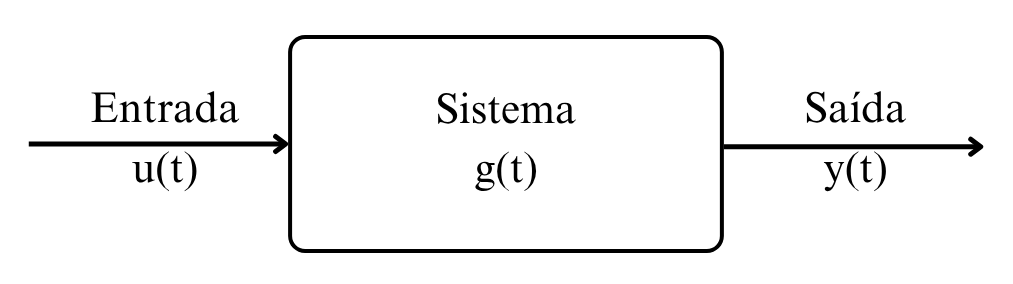
\includegraphics[width=8cm]{figuras/fundamentação-teorica/exemplo-sistema.png}
				}{
					\Fonte{O autor}
				}	
		\end{figure}

		Outra característica a ser considerada dentro dos sistemas estudados tem a ver com a sua linearidade ou não, ou seja, a possibilidade de se aplicar o princípio da superposição no processo analisado, visto que a resposta a diversas entradas simultâneas pode ser entendida como a soma das respostas a cada entrada individualmente \cite{ogata-2010}.

		Processos de velocidade, tais quais os dos motores presentes no \textit{micromouse}, apresentam não linearidades inerentes ao sistema. Porém, como mostrado em \citeonline{dissetacao-pereira-2000}, para o caso dos micro-robôs móveis com equações cinemáticas como as descritas em \ref{eq:vel-linear-global} a \ref{eq:vel-linear-esquerda}, as não linearidades são consideradas fracas de maneira que os parâmetros do modelo ainda são lineares.

		\subsection{Modelagem em domínio contínuo} \label{ssec:modelagem-domniio-continuo}

			Uma forma comum para descrever sistemas consiste na sua modelagem matemática. Assim, supondo que $g(t)$ seja uma função matemática de tempo contínuo capaz de modelar a dinâmica do sistema, e que os sinais de entrada e de saída do sistema, respectivamente $u(t)$ e $y(t)$, possuam suas Transformadas de Laplace $U(s)$ e $Y(s)$, pode se representar o bloco da Figura \ref{fig:sistema-controle-generico} pela equação \ref{eq:funcao-transferencia-generica-s} a qual é definida como \gls{FT} do sistema em tempo contínuo.

			\begin{equation}
				\label{eq:funcao-transferencia-generica-s}
				G(s) = \frac{Y(s)}{U(s)} = \frac{\mathcal{L}\{y(t)\}}{\mathcal{L}\{u(t)\}}
			\end{equation}
			
			A Equação \ref{eq:funcao-transferencia-generica-s} pode ser expandida para a forma da Equação \ref{eq:expansao-ft-s}, onde $b_i$ e $a_i$ são os coeficientes polinomiais de $Y(s)$ e $U(s)$ respectivamente. O sistema pode então ser dito de \textit{ordem n} caso a maior potência do seu denominador seja $n$ \cite{ogata-2010}.

			\begin{equation}
				\label{eq:expansao-ft-s}
				G(s) = \frac{Y(s)}{U(s)} =\frac{b_0 s^m + b_1 s^{m-1} + \cdots + b_{m-1} s + b_m}{a_0 s^n + a_1 s^{n-1} + \cdots + a_{n-1} s + a_n}
			\end{equation}

			Os sistemas na natureza, entretanto, podem ser modelados por \gls{FT} de ordem $2$. Dessa forma, que a Equação \ref{eq:expansao-ft-s} pode ser agora reduzida a Equação \ref{eq:ft-ordem-2-s}.

			\begin{equation}
				\label{eq:ft-ordem-2-s}
				G(s) = \frac{Y(s)}{U(s)} =\frac{b_1 s + b_2}{s^2 + a_1 s + a_2}
			\end{equation}

		\subsection{Modelagem em domínio discreto} \label{ssec:modelagem-domniio-discreto}

			Sistemas computacionais, por sua vez, não são capazes de compreender fenômenos contínuos haja vista que a sua natureza binária e digitalizada não os permite de suportar os infinitos valores em um intervalo finito e real e, portanto, é necessário converter os modelos descritos anteriormente em modelos discretos através da Transformada $Z$. A Transformada $Z$ é aplicada não ao sinal original, mas ao sinal amostrado a partir de um intervalo de tempo $T_s$. 
			
			Assim, dado um sinal genérico $r(t)$ e amostrado no intervalo de tempo $T_s$, conforme a Figura \ref{fig:amostragem-tempo-discreto}, pode-se definir a transformada $Z$ do sinal conforme \citeonline{ibrahim-2006}, pela Equação \ref{eq:definicao-transformada-z}.

			\begin{figure}[htbp]
					\centering
					\Caption{\label{fig:amostragem-tempo-discreto} Amostragem de um sinal contínuo}	
					\UFCfig{}{
						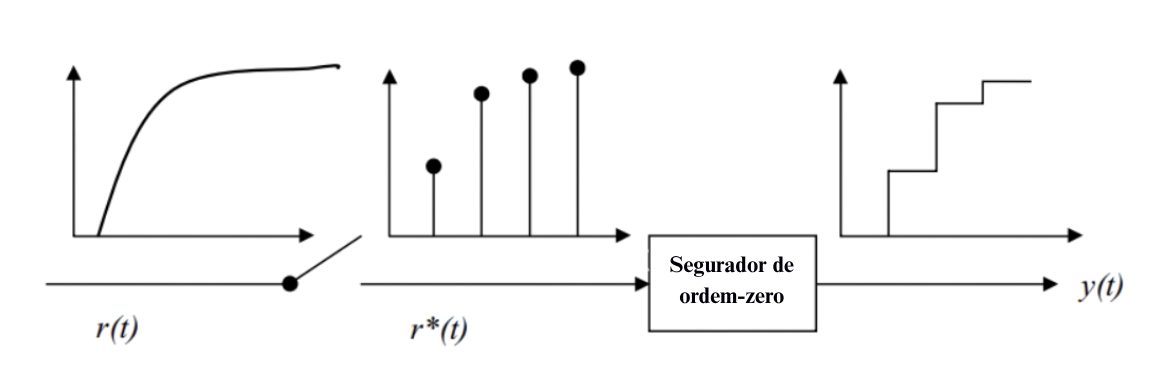
\includegraphics[width=9cm]{figuras/fundamentação-teorica/amostragem-ibrahim.png}
					}{
						\Fonte{\citeonline{ibrahim-2006}}
					}	
			\end{figure}

			\begin{equation}
				\label{eq:definicao-transformada-z}
				Z[r(t)] = R(z) = \sum_{n=0}^{\infty} r(n T_s) z^{-n}
			\end{equation}

			Aplicando a equação anterior na \gls{FT} dos processos de segunda ordem descritos pelo Equação \ref{eq:ft-ordem-2-s}, pode-se obter a \gls{FT} discreta conforme \ref{eq:ft-ordem-2-z}. 

			\begin{equation}
				\label{eq:ft-ordem-2-z}
				G(z) = \frac{Y(z)}{U(z)} = \frac{b_1 z^{-1} + b_2 z^{-2}}{z + a_1 z^{-1} + a_2 z^{-2}}
			\end{equation}

			Em sistemas reais as resposta não são instantâneas, de modo que pode existir um certo intervalo de tempo até que seus efeitos sejam visíveis, e, dessa forma, faz-se necessário considerar o termo do \textit{atraso de transporte}, fazendo com que a forma final usada para modelagem de sistemas dinâmicos seja a Equação \ref{eq:ft-ordem-2-z-com-atraso}.

			\begin{equation}
				\label{eq:ft-ordem-2-z-com-atraso}
				G(z) = \frac{Y(z)}{U(z)} = z^{-d} \frac{b_1 z^{-1} + b_2 z^{-2}}{z + a_1 z^{-1} + a_2 z^{-2}}
			\end{equation}
			
			\noindent
			onde os termos $z^{-1}$, $z^{-2}$ e $z^{-d}$ indicam atrasos de 1, 2 e $d$ \textit{períodos amostragem} respectivamente.

			Assim, a \textit{equação a diferenças} usada para os cálculos computacionais é derivada a partir da \gls{FT} discreta do processo e está explicitada na Equação \ref{eq:equacao-diferencas}.

			\begin{equation}
				\label{eq:equacao-diferencas}
				y[k] = -a_1 y[k-1] - a_2 y[k-2] + b_1 u[k-1-d] + b_2 u[k-2-d]
			\end{equation}

			As Equações \ref{eq:ft-ordem-2-z-com-atraso} e \ref{eq:equacao-diferencas} serão usadas para a construção do vetor de parâmetros para a estimação do modelo.

		\subsection{Estimador dos Mínimos Quadrados Não-Recursivo} \label{ssec:estimador-mqnr}

			O Estimador dos \gls{MQNR} é uma técnica clássica baseada no \textit{Princípio dos Mínimos Quadrados} de Gauss elaborado no século XVIII para prever as trajetórias de planetas a partir da realização de medições e observações \cite{coelho-identificacao}. 
			
			Este método utiliza um vetor de medidas, $\varphi(t)$, a partir de um conjunto de dados extraídos de experimentações para a construção de uma aproximação $\hat{\theta}$ do vetor de parâmetros $\theta(t)$ do qual os elementos são retirados e utilizados diretamente na Equação \ref{eq:equacao-diferencas}.

			O vetor das medidas coletadas, $\varphi(t)$, com dimensão $[(m + n + 1) \times 1]$, é definido pela Equação \ref{eq:vetor-phi-medidas}.

			\begin{equation}
				\label{eq:vetor-phi-medidas}
				\varphi^T(t) = [-y(t-1) \ -y(t-2) \ \ldots \ -y(t-m) \ u(t-d) \ \ldots \ u(t-d-n)]
			\end{equation}

			Já o vetor de parâmetros, $\hat{\theta}$, é:
			\begin{equation}
				\label{eq:vetor-theta-medidas}
				\theta^T(t) = [a_1 \ a_2 \ \ldots \ a_{m} \ b_0 \ b_1 \ \ldots \ b_{n}]
			\end{equation}

			E a representação matricial da saída do sistema é dada por:

			\begin{equation}
				\label{eq:vetor-y-medidas}
				Y = \Phi \theta + E
			\end{equation}

			\noindent
			onde $E$ é o vetor de pertubações e $\Phi$ a matriz para $N$ medidas, dada por \ref{eq:matriz-Phi-medidas}.

			\begin{equation}
				\label{eq:matriz-Phi-medidas}
				\Phi =  \begin{bmatrix}
							\varphi^T(0) \\
							\varphi^T(1) \\
							\vdots \\
							\varphi^T(N-1)
						\end{bmatrix}
			\end{equation}
			
			O critério para obtenção do vetor de parâmetros $\hat{\theta}$ é dado pela resolução da Equação \ref{eq:criterio-minimizacao-mqnr} a qual corresponde à minização do erro de previsão quadrático.

			\begin{equation}
				\label{eq:criterio-minimizacao-mqnr}
				J = \min_{\theta} \left\| Y - \phi \hat{\theta} \right\|_W^2
			\end{equation}

			Assim, resolvendo a equação anterior é possível obter a definição de $\hat{\theta}$.

			\begin{equation}
				\label{eq:estimador-mqnr}
				\hat{\theta} = [\Phi^T \Phi]^{-1} \Phi^T \mathbf{Y}
			\end{equation}

			Para que a estimação dos parâmetros seja a mais precisa possível, \citeonline{dissetacao-pereira-2000} estabelece que a aquisição de dados deve considerar 3 pontos, os quais são:

			\begin{enumerate}
				\item A coleta de dados deve ser em malha aberta para evitar a correlação entre as entradas.
				\item O sistema deve ser excitado de forma a extrair o máximo possível da informação da panta.
				\item A excitação deve ser feita com pequenas variações em torno de um ponto de operação a fim de reduzir o efeito de fenômenos não modelados como não linearidades.
			\end{enumerate}

			Em consonância com o estabelecido acima, \citeonline{aguirre-identificacao-2007} estabelece que o sinal de entrada deve ser um sinal branco. Isto implicará que tal sinal tem energia em uma faixa de frequências ampla e que engloba a faixa de frequências dominantes do sistema que se deseja identificar, ou seja, o sinal branco será capaz de excitar adequadamente a dinâmica da planta, o que pode ser obtido quando a excitação ocorre em torno de um ponto de operação.

			Conjuntamente deve ser observado também que o produto matricial $[\Phi^T \Phi]$, presente na Equação \ref{eq:estimador-mqnr}, deve ser invertível. Assim, supondo o sinal de entrada, $u(t)$, constante e igual a $u_0$, tem-se, para $N$ medidas, que o produto resultará em uma matriz singular no formado de:

			\begin{center}
				$
				[\Phi^T \Phi] = N u_0 
				\begin{bmatrix}
					1 & 1 \\
					1 & 1 \\	
				\end{bmatrix}
				$
			\end{center}

			E, portanto, o sinal de entrada deve possuir variação para garantir que a Equação \ref{eq:determinante-nao-nulo} seja obedecida.

			\begin{equation}
				\label{eq:determinante-nao-nulo}
				\text{det} \left\{ \Phi^T \Phi \right\} \neq 0
			\end{equation}

			Desse modo, a escolha do sinal de entrada adequado é crucial para a correta identificação de sistemas de controle. Um dos sinais mais empregados nesse contexto é o \gls{PRBS}, conforme apresentado por \citeonline{aguirre-identificacao-2007}, \citeonline{coelho-identificacao} e \citeonline{norgaard-2000-neural}, devido à sua capacidade de atender aos requisitos descritos anteriormente.

			% Desse modo a escolha do sinal de entrada adequado é crucial para a correta identificação dos sistemas de controle. Um dos sinais mais comumente empregados nesse contexto são os \gls{PRBS} os quais além de aparecerem em \cite{aguirre-identificacao-2007, coelho-identificacao, dissetacao-pereira-2000} também são apresentados em \citeonline{norgaard-2000-neural} devido à sua capacidade de atender a todos os requisitos descritos anteriormente.

			Sinais \gls{PRBS} são sequências pseudo-aleatórias que podem assumir apenas dois valores em torno de um ponto de operação. Tais sinais são determinísticos, isto é, podem ser gerados novamente diversas vezes, são periódicos com metade mais um dos intervalos em um nível e, metade menos um, em outro nível \cite{aguirre-identificacao-2007}.
			
			Assim, diante do exposto até aqui, o presente trabalho faz uso do referido sinal como sinal de entrada para modelagem dos sistemas dinâmicos presentes no \textit{micromouse}, a saber:

			\begin{itemize}
				\item O robô, quanto ao seu comportamento relativo à sua velocidade linear global, descrito pela Equação \ref{eq:vel-linear-global}.
				\item O robô, quanto ao seu comportamento relativo à sua velocidade angular global, descrito pela Equação \ref{eq:vel-angular-global}.
				\item Os motores de corrente contínua, responsáveis pelas velocidades direita e esquerda do robô, os quais são descritos pelas Equações \ref{eq:vel-linear-direita} e \ref{eq:vel-linear-esquerda}, respectivamente.
			\end{itemize}
				
    \section{Controle de Sistemas Dinâmicos} \label{sec:controle-teoria}

        % \textbf{abordar aqui: relé, astrom, PID e Equações do PID em Z}
		
		De posse do modelo de cada um dos sistemas, elaborados conforme as seções anteriores, é possível proceder para o projeto e desenvolvimento dos controladores. Este trabalho faz uso de controladores do tipo \gls{PID} projetados utilizando o método de {\AA}str{\"o}m com autossintonia pelo Método do Relé. Todo o processo é realizado computacionalmente, ou seja, é feito também o uso da \textit{Transformada Z} descrita em \ref{eq:definicao-transformada-z}.

		\subsection{Controlador Proporcional-Integral-Derivativo} \label{ssec:teoria-pid}

			Até agora, os sistemas considerados encontravam-se em \gls{MA}, como o exemplo mostrado na Figura \ref{fig:sistema-controle-generico}, isto é, era aplicado um sinal de entrada $u(t)$ e era observado o comportamento da saída $y(t)$. Entretanto, controlar um sistema significa forçar o seu comportamento final para um comportamento desejado de forma que, na maioria das vezes, isso deve ser realizado com a utilização de uma realimentação, o que qualifica o sistema agora como em \gls{MF}, pois está presente, também, um sinal de referência $r(t)$ e um sinal de erro $e(t)$ definido como:

			\begin{equation}
				\label{eq:definicao-erro}
				e(t) = r(t) - y(t)
			\end{equation}

			A Figura \ref{fig:sistema-malha-fechada-simples} exemplifica um sistema em \gls{MF} e a Figura \ref{fig:sistema-malha-fechada-controlador} exemplifica um sistema em \gls{MF} controlado. A partir da Figura \ref{fig:sistema-malha-fechada-controlador} pode-se observar que o controlador irá atuar em cima do erro $e(t)$ de forma que o objetivo é zerar o valor desse sinal.

			\begin{figure}[htpb]
				\centering
				\Caption{\label{fig:sistema-malha-fechada-simples} Sistema em Malha Fechada}
				\UFCfig{}{
					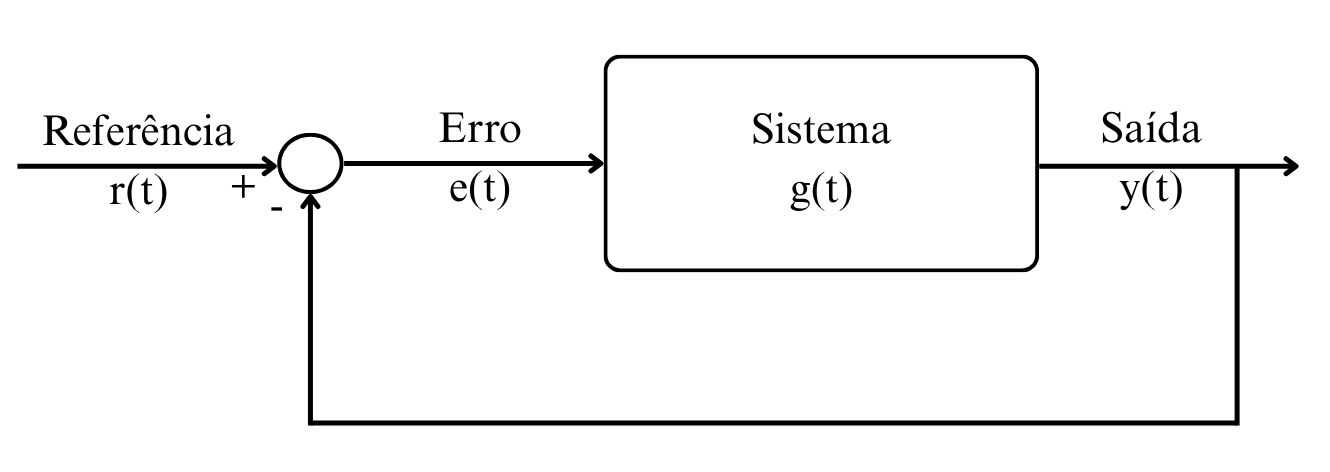
\includegraphics[width=12cm]{figuras/fundamentação-teorica/sistema-mf-simples.png}
				}{
					\Fonte{O autor}
				}	
			\end{figure}

			\begin{figure}[htpb]
				\centering
				\Caption{\label{fig:sistema-malha-fechada-controlador} Sistema em Malha Fechada com Controlador}
				\UFCfig{}{
					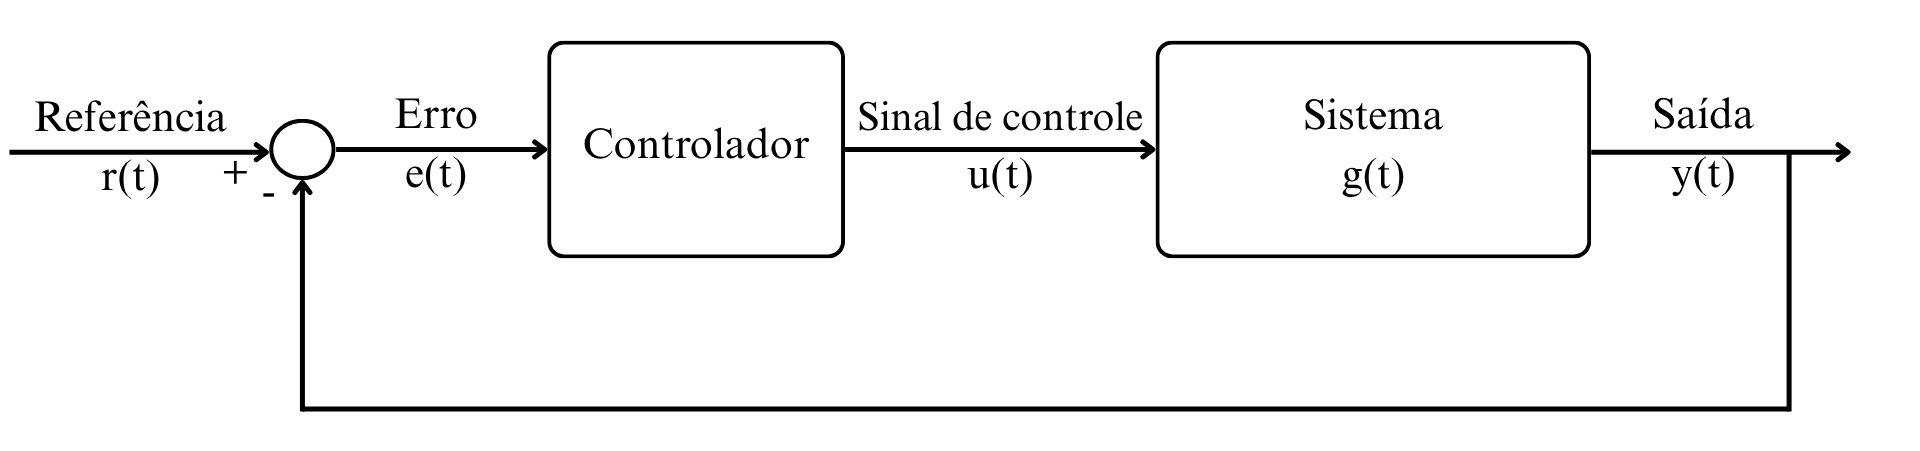
\includegraphics[width=12cm]{figuras/fundamentação-teorica/sistema-mf-controlado.png}
				}{
					\Fonte{O autor}
				}	
			\end{figure}
			
			Assim, o controlador \gls{PID}, definido pela Equação \ref{eq:definicao-pid-tempo}, é composto de três tipos básicos de ação de controle: a ação proporcional, a ação integrativa e a ação derivativa. A ação proporcional consiste em um ganho (chamado de ganho proporcional) simples aplicado ao erro, visando reduzir valor do \textit{erro de regime permanente}. A ação integrativa consiste em um ganho (ganho integrativo) aplicado à soma do erro em um intervalo de tempo $t$, seu objetivo é zerar o \textit{erro de regime permanente}. Por fim, a ação derivativa consiste em um ganho (ganho derivativo) aplicado à taxa de variação do erro em um intervalo de tempo $t$, cujo objetivo é corrigir problemas no transitório da resposta do sistema. 
			
			\begin{equation}
				\label{eq:definicao-pid-tempo}
				u(t) = K_p e(t) + K_i \int_0^t e(t) \, dt + K_d \frac{de(t)}{dt}
			\end{equation}

			\noindent
			onde $K_p$, $K_i = \frac{K_p}{T_i}$ e $K_d = K_p T_d$ são os ganhos proporcional, integrativo e derivativo respectivamente. $T_i$ representa o tempo de integrativo e $T_d$ representa o tempo de derivativo. E, aplicando a \textit{Transformada de Laplace} na equação anterior, é possível obter a \gls{FT} em $s$ de um controlador \gls{PID}.

			\begin{equation}
				\label{eq:definicao-pid-laplace}
				G_c(s) = \frac{U(s)}{E(s)} = K_p \left( 1 + \frac{1}{T_i s} + T_d s \right)
			\end{equation}
			
			Assim, ao aplicar-se a \textit{Transformada Z}, para uma amostragem com um período de amostragem $T_s$, na Equação \ref{eq:definicao-pid-laplace}, obtêm-se a \gls{FT} em $z$ de um controlador \gls{PID}, a qual é definida por:

			\begin{equation}
				\label{eq:definicao-pid-z}
				G_c(z) = \frac{U(z)}{E(z)} = \frac{g_0 z^2 + g_1 z + g_2}{z(z-1)}
			\end{equation}

			\noindent
			onde,

			\begin{center}
				$g_0 = K_p + \frac{K_i T_s}{2} + \frac{K_d}{T_s}$ \\
				$g_1 = \frac{K_i T_s}{2} - K_p - \frac{2 K_d}{T_s}$ \\
				$g_2 = \frac{K_d}{T_s}$
			\end{center}

			E, por fim, a equação a diferenças do controlador \gls{PID} obtida a partir de \ref{eq:definicao-pid-z} é:

			\begin{equation}
				\label{eq:equaca-diferenca-pid}
				u[k] = g_0 e[k] + g_1 e[k-1] + g_2 e[k-2] + u[k-1]
			\end{equation}

			De posse das equações acima, o passo seguinte é sintonizar os parâmetros $K_p$, $T_i$ e $T_d$.

		\subsection{Sintonia pelo Método do Relé} \label{sec:autossintonia-rele}

			A escolha dos parâmetros do controlador \gls{PID} não é um processo trivial ou intuitivo e, a depender da abordagem escolhida, demanda testes experimentais (podendo ser simulados com o uso do modelo) ou um desenvolvimento matemático analítico mais completo. Técnicas clássicas já consolidadas na academia e no ambiente industrial existem, e as mais comuns são, por exemplo, as desenvolvidas por \citeonline{ziegler-nichols-1942}. Posteriormente, é possível citar também \citeonline{yu-2006-relay} e \citeonline{astrom-1995}.

			% O Método do Relé usado na parametrização de controladores se utiliza da resposta de retorno de um relé para provocar uma oscilação sustentada em um sistema e é considerado um avanço das técnicas convencionais de \citeonline{ziegler-nichols-1942} em especial o segundo método. Entre as suas vantagens está a possibilidade de parametrização sem necessariamente obter-se um modelo da planta. Além disso, por ser um teste em malha fechada evitará desvios das condições nominais de operação e, ainda, é mais eficiente que métodos convencionais como os testes de resposta ao impulso e resposta ao degrau \cite{yu-2006-relay}.

			O Método do Relé, baseia-se na inserção de um relé na malha de controle para induzir oscilações sustentadas no sistema. A partir da análise dessas oscilações é possível determinar parâmetros relevantes para o ajuste do controlador. Esse método é considerado uma evolução das técnicas clássicas propostas por \citeonline{ziegler-nichols-1942}, especialmente do segundo método de sintonia, que utiliza o ganho crítico e o período de oscilação do processo. 
			
			Entre as principais vantagens, pode-se destacar a possibilidade de realizar a parametrização sem a necessidade de obter previamente um modelo matemático da planta. Ademais, por ser conduzido em \gls{MF}, o ensaio mantém o sistema próximo de suas condições normais de operação, reduzindo desvios significativos do ponto de funcionamento. Outra característica importante é sua maior eficiência quando comparado a métodos convencionais de identificação, como os testes de resposta ao impulso e resposta ao degrau \cite{yu-2006-relay}.

			As figuras \ref{fig:diagrama-bloco-rele} e \ref{fig:sinal-saida-rele} a seguir representam, respectivamente, o diagrama de blocos com a inserção do relé e o sinal oscilatório que se busca gerar com a utilização desse método.

			\begin{figure}[htb]
				\centering
				\Caption{\label{fig:diagrama-bloco-rele} Diagrama de Blocos com o Relé}
				\UFCfig{}{
					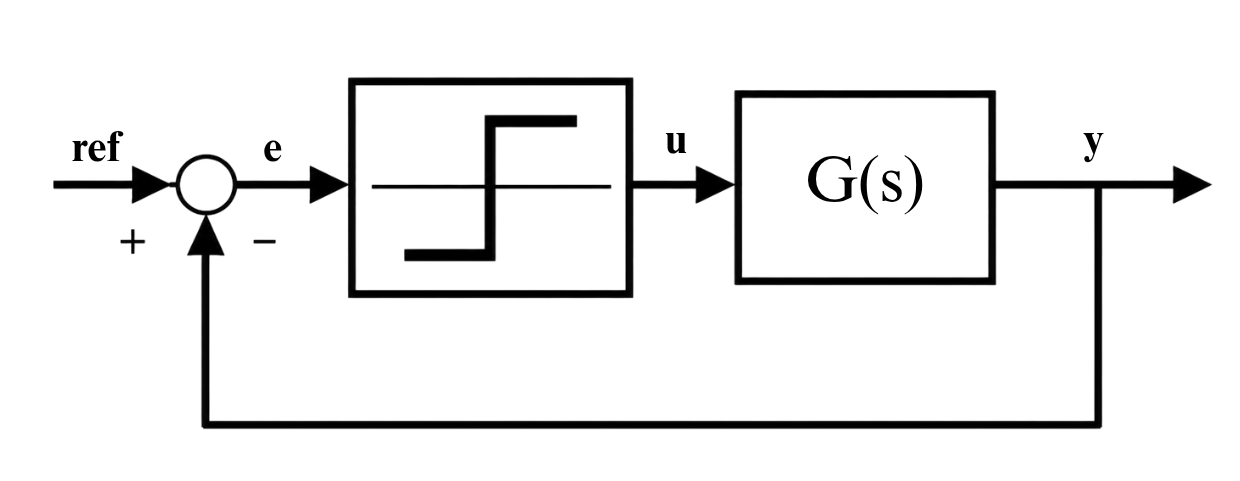
\includegraphics[width=9cm]{figuras/fundamentação-teorica/block-diagram-relay.png}
				}{
					\Fonte{O autor}
				}	
			\end{figure}

			\begin{figure}[htb]
				\centering
				\Caption{\label{fig:sinal-saida-rele} Resposta desejada com o uso do Relé}
				\UFCfig{}{
					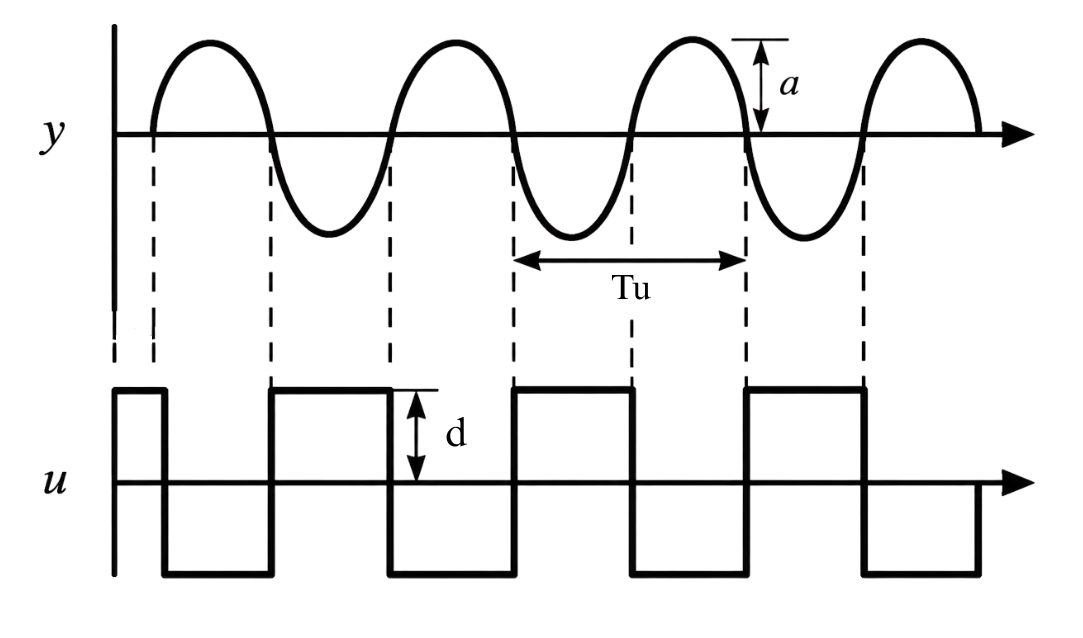
\includegraphics[width=9cm]{figuras/fundamentação-teorica/output-relay.png}
				}{
					\Fonte{O autor}
				}	
			\end{figure}

			Tradicionalmente, o segundo método de \gls{ZN} propõe a adição de um bloco Controlador Proporcional no diagrama da Figura \ref{fig:sistema-malha-fechada-controlador} para que com o aumento do ganho $K_p$ o sistema apresente oscilações até o momento em que atinja o limiar de estabilidade, ou seja, fique completamente oscilatório e nesse momento o valor do ganho atinge seu valor que é dito \textit{crítico} (ou último), $K_u$. São medidos, também, o período da oscilação, $T_u$, e a frequência de oscilação $\omega_u$. 
			
			De posse dessas medidas tal método propõe a utilização da Tabela \ref{tab:zn2-parametros} para a determinação dos valores de $K_p$, $T_i$ e $T_d$. Todavia, em diversos processos, a aplicação direta do método descrito anteriormente não é viável, uma vez que as condições operacionais não permitem o aumento progressivo do ganho até que se atinja o \textit{ganho crítico}.

			\begin{table}[!htbp]	
				\centering
				\Caption{\label{tab:zn2-parametros} Sintonia de controladores \gls{PID} pelo segundo método de \gls{ZN}}
				\UFCtab{}{
					\begin{tabular}{cccc}
						\toprule
						Tipo de controlador & \( K_p \) & \( T_i \) & \( T_d \) \\
						\midrule
						P    & \( 0,5 K_{u} \) & \( \infty \) & \( 0 \) \\
						PI   & \( 0,45 K_{u} \) & \( \frac{1}{1,2} T_{u} \) & \( 0 \) \\
						PID  & \( 0,6 K_{u} \) & \( 0,5 T_{u} \) & \( 0,125 T_{u} \) \\
						\bottomrule
					\end{tabular}
				}{
					\Fonte{\citeonline{ogata-2010}}
				}
			\end{table}

			% Todavia, em diversos processos não é possível a aplicação direta do método acima descrito haja vista que as condições operacionais não permitirão ao aumento progressivo do ganho até se alcançar o \textit{ganho crítico}. Dessa forma, {\AA}str{\"o}m e H{\"a}gglund propõem a utilização de um relé para se alcançar tais parâmetros. E, assim, quando este é introduzido, o sistema passa automaticamente a oscilar com período $T_u$ e freqûencia $\omega_u$ as quais possuem a seguinte relação: 
			
			% \citeonline{astrom-1995} observaram que com a introdução de um relé de amplitude $d$, na malha de controle, o sistema produz uma saída oscilatória de amplitude $a$ (Figura \ref{fig:sinal-saida-rele}), automaticamente, com período $T_u$ e frequência $\omega_u$, os quais estão relacionados conforme a equação \ref{eq:relacao-periodo-frequencia}. O valor do \textit{ganho crítico}, por sua vez, está relacionado com a amplitude do relé e com a amplitude do sinal de saída, conforme a equação \ref{eq:ganho-critico-rele}. 
			
			\citeonline{astrom-1995} observaram que a introdução de um relé de amplitude $d$ na malha de controle faz com que o sistema produza automaticamente uma saída oscilatória com amplitude $a$ (Figura \ref{fig:sinal-saida-rele}). Essas oscilações ocorrem com período $T_u$ e frequência $\omega_u$, relacionadas pela Equação \ref{eq:relacao-periodo-frequencia}. Além disso, o valor do \textit{ganho crítico} está diretamente relacionado à amplitude do Relé e à amplitude do sinal de saída, conforme expresso na Equação \ref{eq:ganho-critico-rele}.


			\begin{equation}
				\label{eq:relacao-periodo-frequencia}
				\omega_u = \frac{2 \pi}{T_u}
			\end{equation}

			\begin{equation}
				\label{eq:ganho-critico-rele}
				K_u = \frac{4 d}{\pi a}
			\end{equation}

			% Assim, considerando a curva de Nyquist pode-se entender o Relé como sendo o elemento que desloca um ponto na curva característica do processo para uma posição desejada. É possível, ainda, considerar uma histerese $\epsilon$ para que o ponto na curva seja deslocado no plano complexo.

			Considerando o diagrama de \textit{Nyquist}, o Relé pode ser interpretado como um elemento que desloca o ponto de operação associado à oscilação para uma posição específica na curva característica do processo. Além disso, é possível introduzir uma histerese $\varepsilon$, modificando sua característica de chaveamento. A presença dessa histerese permite deslocar o ponto correspondente na curva de \textit{Nyquist} para uma nova posição no plano complexo, ampliando a flexibilidade do método na obtenção das informações dinâmicas do processo. Dessa forma, é possível explorar diferentes regiões da curva característica, possibilitando uma manipulação mais abrangente do comportamento do sistema. 
			
			A Equação característica do \textit{Relé com Histerese}, \ref{eq:equacao-rele-histerese}, a seguir, mostra que o sem a histerese ($\varepsilon = 0$) o ponto da curva de \textit{Nyquist} se encontrava em cima do eixo real, em seu lado negativo. Com ela o ponto passa a ser deslocado agora para o $3^\circ$ quadrante do plano complexo.

			\begin{equation}
				\label{eq:equacao-rele-histerese}
				G(j \omega) = -\frac{1}{N(a)} = -\frac{\pi}{4d} \sqrt{a^2 - \varepsilon^2} - j \frac{\pi \varepsilon}{4d}
			\end{equation}

			\noindent
			onde, 

			\begin{equation*}
				\begin{cases}
					\operatorname{Re}\{G(j \omega)\} = -\dfrac{\pi}{4d} \sqrt{a^2 - \varepsilon^2} \\[10pt]
					\operatorname{Im}\{G(j \omega)\} = -\dfrac{\pi \varepsilon}{4d}
				\end{cases}
			\end{equation*}

			O ponto encontrado pode ser então descrito pelo seu módulo $R_a$ e sua fase $\phi_a$ dados pelas Equações \ref{eq:modulo-rele} e \ref{eq:fase-rele}, respectivamente.

			\begin{equation}
				\label{eq:modulo-rele}
				R_a = \sqrt{(\operatorname{Re}\{G(j \omega)\})^2 - (\operatorname{Im}\{G(j \omega)\})^2}
			\end{equation}

			\begin{equation}
				\label{eq:fase-rele}
				\phi_a = \arctan \left( \frac{\operatorname{Im}\{G(j \omega)\}}{\operatorname{Re}\{G(j \omega)\}} \right)
			\end{equation}

			O controlador \gls{PID}, descrito pela Equação \ref{eq:definicao-pid-laplace} provoca um novo deslocamento em fase e módulo do ponto na curva de \textit{Nyquist}, encontrando um novo ponto agora com módulo $R_b$ e fase $\phi_b$. À variação sofrida dá-se o nome, respectivamente, de margem de fase $\phi_m$ e margem de ganho $A_m$ os quais podem ser descritos pelas Equações \ref{eq:margem-fase} e \ref{eq:margem-ganho}.

			\begin{equation}
				\label{eq:margem-fase}
				\phi_m = \phi_b - \phi_a
			\end{equation}

			\begin{equation}
				\label{eq:margem-ganho}
				A_m = \frac{R_b}{R_a}
			\end{equation}

			E assim, os parâmetros de controle $K_p$, $T_i$ e $T_d$ podem ser definidos conforme \citeonline{astrom-1984} em função dos elementos já apresentados e de um novo valor $\alpha$.

			\begin{equation}
				\label{eq:parametro-kp}
				K_p = \frac{K_u}{A_m} \cos \phi_m
			\end{equation}

			\begin{equation}
				\label{eq:parametro-td}
					T_d = \frac{\tan \phi_m + \sqrt{\frac{4}{\alpha} + \tan^2 \phi_m}}{2 \omega_u}
			\end{equation}

			\begin{equation}
				\label{eq:parametro-ti}
				T_i = \alpha T_d
			\end{equation}

			Dessa forma, serão projetados controladores do tipo \gls{PID} para o robô \textit{micromouse}, considerando os processos anteriormente descritos. A partir dos parâmetros obtidos pelos métodos de sintonia apresentados, busca-se determinar ajustes adequados para cada malha de controle, de modo a atender aos requisitos de desempenho necessários para o sistema.

%%%%%%%%%%%%%%%%%%%%%%%%%%%%%%%%%%%%%%%%%%%%%%%%%%%%%%%%%%%%%%%%%%%%%%%%%%%%%%%%%%%%%%%%%%%%%%%%%%%%%%%%%%%%%%%%%%%%%%%%%%%%%%%%%%%%%%

\chapter{O Micromouse}
\label{cap:micromouse}

Os robôs móveis têm obtido mais relevância nas últimas décadas com o aprimoramento da microeletrônica e da programação. Estes robôs consistem em sistemas embarcados com microcontroladores e diversos tipos de sensores para se obter as mais variadas informações, sendo os mais comuns os que trabalham com distância, velocidade e angulação. Os sensores podem, ainda, ser classificados em dois grupos: os sensores internos, os quais ficam na própria planta, e os sensores externos, colocados no ambiente de atuação do robô \cite{dissetacao-pereira-2000}.


    \section{Características Construtivas} \label{sec:caracteristicas-construtivas}
		Conforme apresentado em \citeonline{manual-microumouse-2015} o robô \textit{$\mu$MaRT Lite Plus} faz parte de um kit de aprendizado de robótica, dispondo do microcontrolador STM32F405RGT6. O robô, que daqui para frente será chamado apenas de \textit{micromouse}, dispõe ainda de 3 botões, sendo um botão de \textit{boot}, um de \textit{reset} e um botão configurável, além de sensores de linha (oito ao total), sensores de parede (quatro ao total), um conector \gls{USB}, um conector \gls{UART}, dois motores com um \textit{encoder} cada, \textit{buzzer} para sinalização sonora, medição de tensão de bateria, um giroscópio para medir a orientação do robô e duas chaves Liga/Desliga sendo uma geral e uma para os motores. A Figura \ref{fig:micromouse-composicao} apresenta uma vista superior do micromouse e da sua composição.
        
		\begin{figure}[htbp]
                \centering
                \Caption{\label{fig:micromouse-composicao} Estrutura e composição do \textit{micromouse}}	
                \UFCfig{}{
                    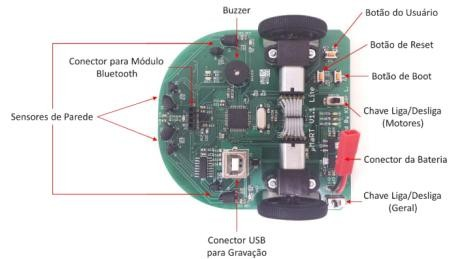
\includegraphics[width=14cm]{figuras/fundamentação-teorica/composicao_micromouse.jpg}
                }{
                    \Fonte{\citeonline{manual-microumouse-2015}}
                }	
        \end{figure}

		\subsection{Programação e Bootloader} \label{ssec:programacao-e-bootloader}
			A programação e gravação dos códigos embarcados (\textit{bootloader}) no robô \textit{micromouse} seguem conforme instruções do desenvolvedor em \citeonline{manual-config-bootloader}, \citeonline{manual-criacao-arm-project}, \citeonline{manual-config-eclipse}  e \citeonline{manual-microumouse-2015}.

	\section{Cinemática} \label{sec:cinematica-micromouse}
		Uma característica fundamental para entender o comportamento do \textit{micromouse} é a sua tração diferencial, isto é, devido ao movimento independente dos seus motores, a sua posição e velocidade global será definida pela diferença de velocidade entre as rodas esquerda e direita. A Figura \ref{fig:movimento-diferencial-micromouse} a seguir ilustra o comportamento descrito anteriormente.

		\begin{figure}[htbp]
                \centering
                \Caption{\label{fig:movimento-diferencial-micromouse} Comportamento diferencial do \textit{micromouse}}	
                \UFCfig{}{
                    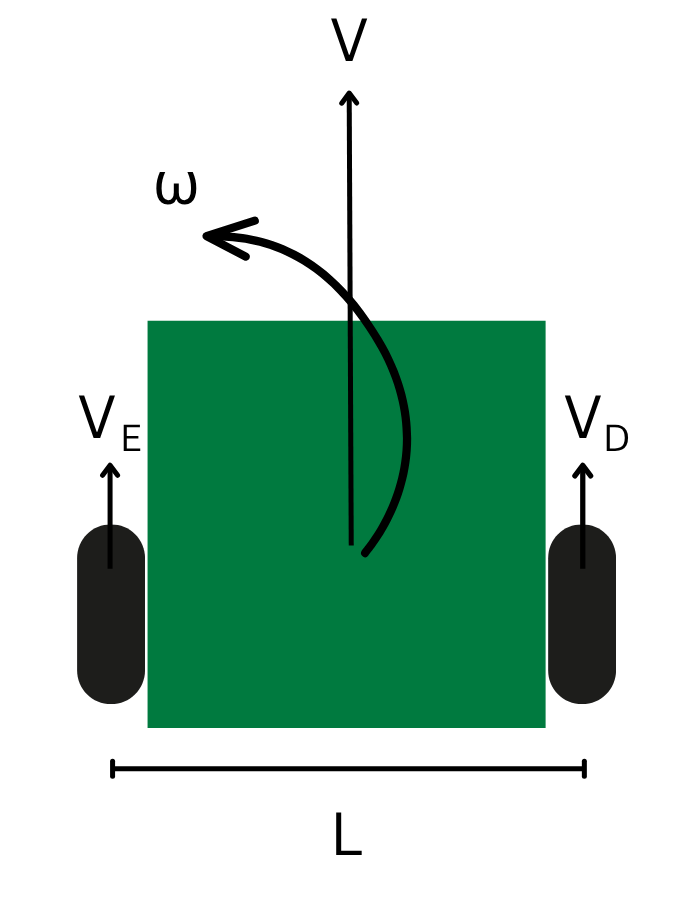
\includegraphics[width=5cm]{figuras/fundamentação-teorica/mov-diferencial-micromouse-puro.png}
                }{
                    \Fonte{O autor}
                }	
        \end{figure}

		Dessa forma a velocidade linear global (\textit{V}) e a velocidade angular global ($\omega$) podem ser calculadas a partir das Equações \ref{eq:vel-linear-global} e \ref{eq:vel-angular-global} e estão apresentadas no formato das Equações \ref{eq:vel-linear-direita} e \ref{eq:vel-linear-esquerda}.

		\begin{equation}
			\label{eq:vel-linear-global}
			V = \frac{V_D + V_E}{2}
		\end{equation}

		\begin{equation}
			\label{eq:vel-angular-global}
			\omega = \frac{V_D - V_E}{L}
		\end{equation}

		\begin{equation}
			\label{eq:vel-linear-direita}
			V_D = \frac{2V + L\omega}{2}
		\end{equation}

		\begin{equation}
			\label{eq:vel-linear-esquerda}
			V_E = \frac{2V - L\omega}{2}
		\end{equation}

		Assim, pode-se notar que as velocidades dependem diretamente da geometria do robô de forma que algumas considerações devem ser feitas:

		\begin{alineas}
			\item Os modelos apresentados nas Equações \ref{eq:vel-linear-global}, \ref{eq:vel-angular-global} não são a única forma de modelar a cinemática do robô. \citeonline{deshmukh-hasamnis-2023}, por exemplo, utilizam um modelo ligeiramente diferente considerando uma nova variável \textbf{R} (raio do centro instatâneo da curva) no denominador das equações citadas;
			
			\item O modelo apresentado em \ref{eq:vel-angular-global} considera o sentido \textbf{positivo} de giro sendo o sentido \textbf{anti-horário};
		\end{alineas}

		Assim, o comportamento cinemático do micromouse, pode ser representado em um diagrama de blocos, ilustrado a seguir na Figura \ref{fig:diagrama-blocos-micromouse}.

		\begin{figure}[htbp]
                \centering
                \Caption{\label{fig:diagrama-blocos-micromouse} Diagrama de blocos da cinemática do \textit{micromouse}}	
                \UFCfig{}{
                    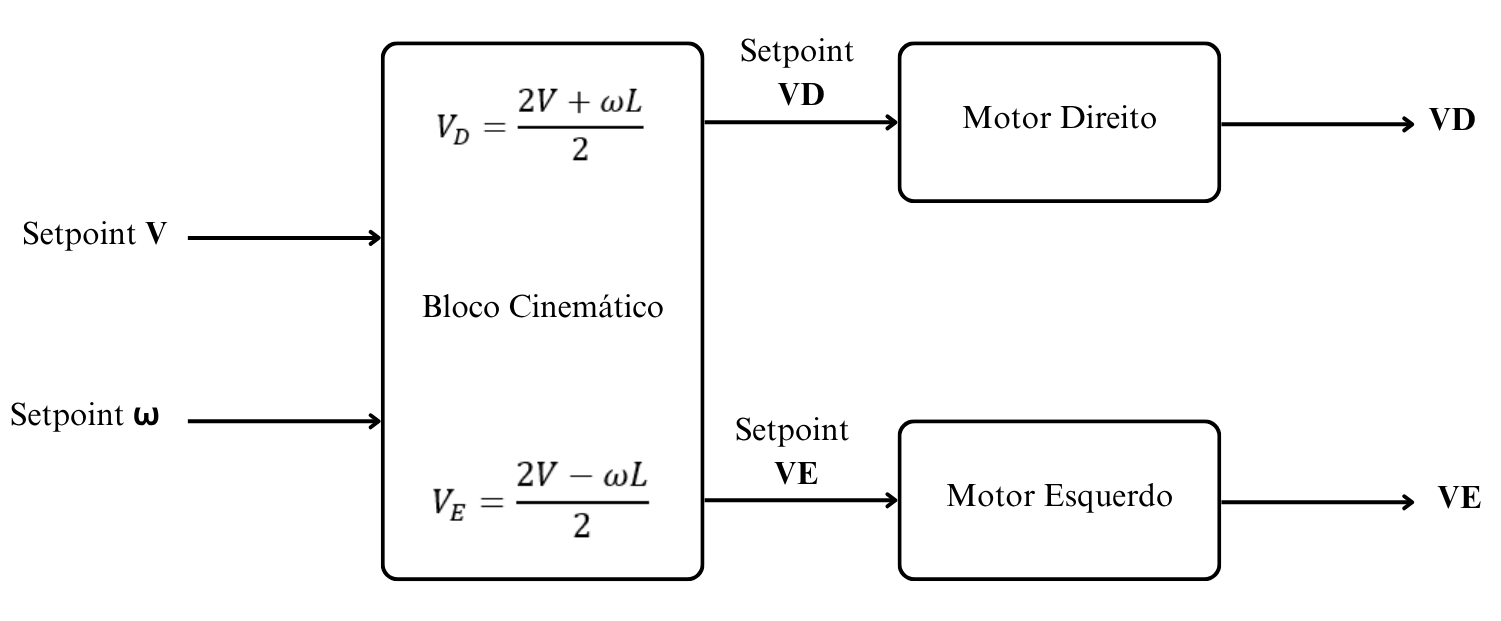
\includegraphics[width=12cm]{figuras/fundamentação-teorica/diagrama-bloco-micromouse.png}
                }{
                    \Fonte{O autor}
                }	
        \end{figure}

	\section{Posicionamento e Orientação} \label{sec:posicionamento-e-orientacao}
		
		Um aspecto imprescindível para a realização do rastreio de trajetórias é o conhecimento sobre a posição atual do robô \textit{micromouse} em cada instante de amostragem de forma a fornecer informações para correções da movimentação. Como no presente trabalho não se dispõe de mecanismos de supervisão externa para acompanhamento, como ocorre em \citeonline{dissetacao-pereira-2000}, tais informações devem ser obtidas com os dados fornecidos pelos sensores do robô e as equações pertinentes de posicionamento devem ser desenvolvidas a partir das equações cinemáticas anteirores.

		De posse das Equações \ref{eq:vel-linear-global} a \ref{eq:vel-linear-esquerda} pode-se obter a representação matricial da cinemática do robô, dada pela Equação \ref{eq:matriz-cinematica-micromouse} onde $\dot{x}_c$, $\dot{y}_c$ e $\dot{\theta}$ representam as variações de posição na direção $x$, $y$ e a variação de orientação $\theta$ respectivamente, como indicado em \ref{fig:micromouse-plano-cartesiano}.

		\begin{equation}
			\label{eq:matriz-cinematica-micromouse}
			\begin{bmatrix}
			\dot{x}_c \\
			\dot{y}_c \\
			\dot{\theta}
			\end{bmatrix}
			=
			\begin{bmatrix}
			\cos\theta & 0 \\
			\sin\theta & 0 \\
			0 & 1
			\end{bmatrix}
			\begin{bmatrix}
			v \\
			\omega
			\end{bmatrix}
		\end{equation}

		\begin{figure}[htbp]
			\centering
			\Caption{\label{fig:micromouse-plano-cartesiano} Deslocamento no plano cartesiano do \textit{micromouse}}	
			\UFCfig{}{
				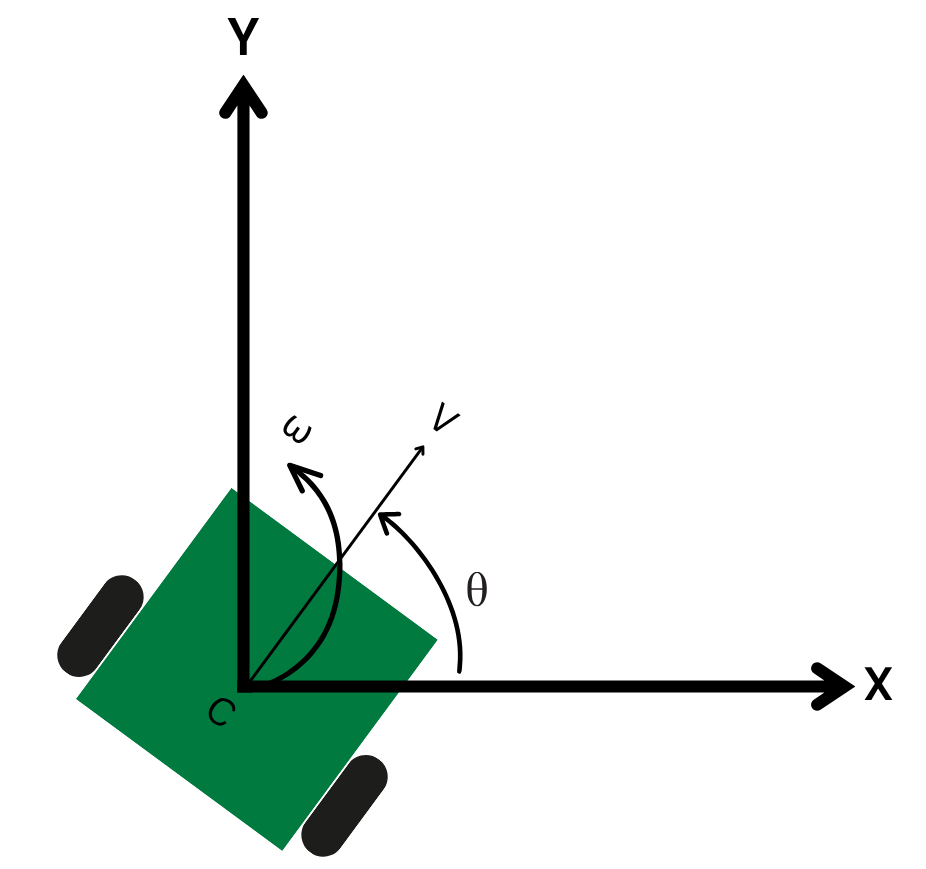
\includegraphics[width=4cm]{figuras/fundamentação-teorica/micromouse-no-plano.png}
			}{
				\Fonte{O autor}
			}	
		\end{figure}

		% Assim, estabelece-se a restrição de movimento do robô \textit{micromouse}, a chamada restrição \textbf{não-holonômica}, a qual implica que o robô não pode se mover em qualquer direção, ou seja, mecanicamente implica queele não pode se descolcar com velocidade perpendicular à posição das suas rodas. A restrição não-holonômica é definida pela equação \ref{eq:restricao-nao-holonomica}.

		Assim é estabelecida a restrição de movimento característica do robô \textit{micromouse}, denominada restrição \textbf{não holonômica}. Essa restrição decorre da configuração do robô diferencial e implica que seu movimento não pode ser realizado de forma arbitrária em todas as direções do plano. 
		
		Em termos físicos, isso significa que o robô não é capaz de desenvolver velocidade lateral instantânea, ou seja, não pode se deslocar perpendicularmente ao plano de rotação de suas rodas sem que haja previamente uma mudança em sua orientação. Dessa forma, seus movimentos ficam limitados às direções compatíveis com sua estrutura mecânica e com as condições de rolamento impostas pelas rodas \cite{vieira-2005}. 
		
		Matematicamente, essa restrição é descrita pela equação \ref{eq:restricao-nao-holonomica}.
		
		\begin{equation}
			\label{eq:restricao-nao-holonomica}
			\dot{x}\,\sin(\theta) - \dot{y}\,\cos(\theta) = 0
		\end{equation}

	\chapter{Metodologia}
\label{cap:metodologia}

% Neste capítulo será apresentada a metodologia utilizada para o desenvolvimento do trabalho. Estruturada da seguinte maneira: na seção \ref{sec:preparacao}, serão apresentados os aspectos relacionados a preparo do robô para a realização de experimentos; na seção \ref{sec:coleta-dados} será abordada a questão de como realizar a coleta de dados para identificação e controle; na seção \ref{sec:id-controle-classico-metodologia}, será apresentada a abordagem utilizada para realização da identificação e controle do robô \textit{micromouse}.

A metodologia utilizada para o desenvolvimento do trabalho foi estruturada em quatro etapas. Inicialmente foram realizados estudos para a adequação do robô \textit{micromouse} disponível no Laboratório de Controle e Automação do \gls{GRASI} do curso de Engenharia Elétrica da \gls{UFPI}. Em seguida, foram realizados estudos e alterações ao nível de \textit{software} para o desenvolvimento da telemetria e do controle do robô. A etapa seguinte consistiu no desenvolvimento dos algoritmos de controle e de identificação para o robô \textit{micromouse}. Por fim, foram executados testes para avaliação das soluções adotadas.

    \section{Preparação inicial} \label{sec:preparacao}
    
        Para a execução de um percurso o mais próximo possível ao ideal, é necessário que o micromouse tenha seus componentes operando, também, o mais próximo da idealidade. Assim, são necessárias serem feitas manipulações mecânicas, e também de software, no robô. 
        
        \subsection{Manipulação mecânica} \label{ssec:manipulacao-mecanica}
            As alterações mecânicas, por sua vez, consistiram em trocar as rodas originais que se encontravam danificadas por rodas semelhantes, porém modeladas e impressas em 3D. A vantagem principal se dá pelo fato de ao possuir um modelo tridimensionald da roda é possível realizar novas impressões em caso de danos causados a estrutura original dessas, com um custo menor que em caso de substituição por peças originais. 
            
            As Figuras \ref{fig:modelo_roda_3d} e \ref{fig:roda_impressa_3d}, a seguir, apresentam, respectivamente, o modelo 3D das rodas originais e a novas impressas.

            \begin{figure}[htbp]
                \centering
                \begin{minipage}{0.45\textwidth}
                    \centering
                    \Caption{\label{fig:modelo_roda_3d} Modelo 3D}
                    %\centering
                    \UFCfig{}{
                        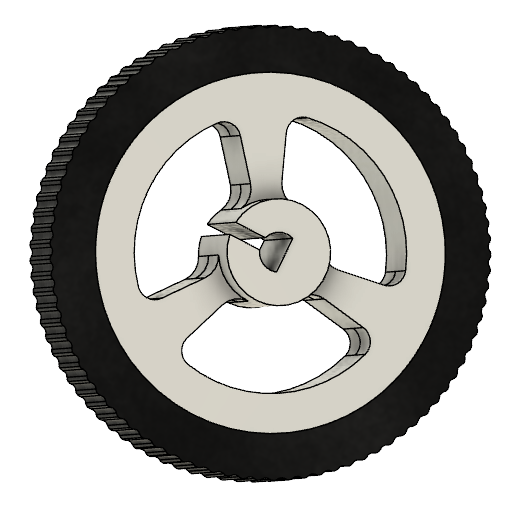
\includegraphics[width=4cm]{figuras/metodologia/modelo_3d_roda.png}
                    }{
                        \Fonte{O autor}
                    }	
                \end{minipage}
                \hfill
                \begin{minipage}{0.45\textwidth}
                    \centering
                    \Caption{\label{fig:roda_impressa_3d} Roda Impressa}
                    %\centering
                    \UFCfig{}{
                        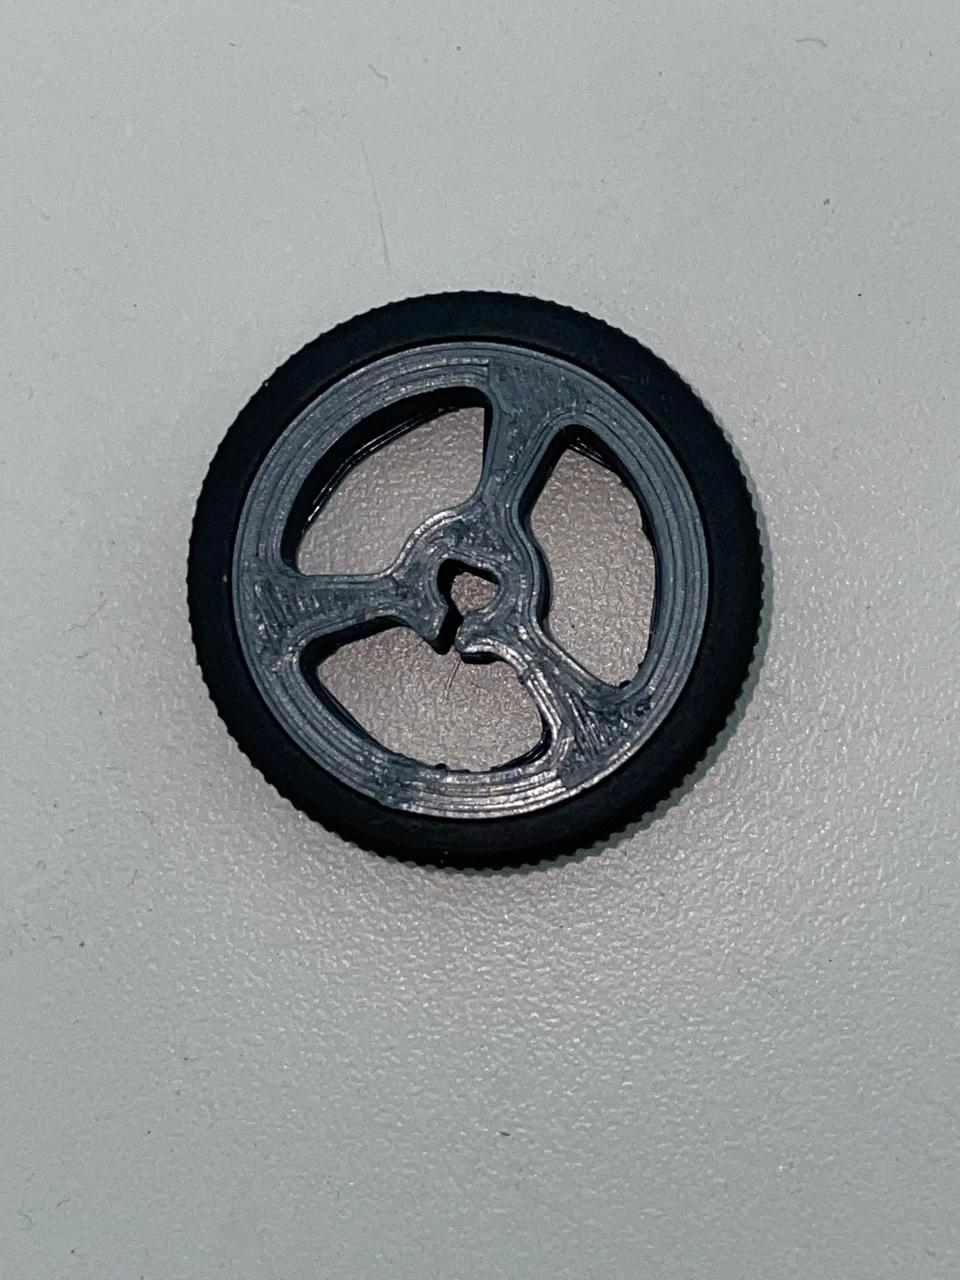
\includegraphics[width=4cm]{figuras/metodologia/roda_impressa.jpg}
                    }{
                        \Fonte{O autor}
                    }	
                \end{minipage}
            \end{figure}
        
        \subsection{Manipulação de software} \label{ssec:manipulacao-sowftware}
            As alterações via software correspondem à programação desenvolvida e embarcada no microcontrolador. No presente trabalho pode-se destacar 3 ferramentas de produção de código utilizadas. São elas as seguintes \gls{IDE} (sigla em inglês para Ambiente de Desenvolvimento Integrado): \gls{VSCode}, MATLAB e Eclipse IDE.

            O \gls{VSCode}, é um editor de códigos desenvolvido pela \textit{Microsoft} que pode ser utilizado com diferentes linguagens de programação, entre elas linguagens C e C++, as quais foram usadas para programar os microcontroladores ESP32 e ESP8266, abordada em \ref{ssec:comunicacao}.

            O MATLAB, por sua vez, é uma \gls{IDE} e uma linguagem de programação com foco em computação numérica e análise de dados \cite{matlab-def}. Esse ambiente foi utilizado para recebimento dos dados e para desenvolvimento dos algorítmos de identificação bem como para obtenção dos parâmetros dos controladores posteriormente embarcados no robô.

            Por fim, o Eclipse IDE foi usado na sua versão para sistemas embarcados (\textit{for Embedded  C/C++ Developers}) para produção dos códigos que a serem embarcados no \textit{micromouse}. Esta versão, conforme \citeonline{eclipse-def}, possui plug-ins de compilação cruzada (\textit{cross build}) e de suporte a arquiteturas ARM e RISC-V.

            % A seguir são apresentadas, nas figuras \ref{fig:vscode-interface}, \ref{fig:matlab-interface} e \ref{fig:eclipse-interface}, respectivamente, as interfaces do \gls{VSCode}, do MATLAB e do Eclipse IDE.


            % \begin{figure}[htbp]
            %     \centering
            %     \Caption{\label{fig:vscode-interface} Interface do \gls{VSCode}}	
            %     \UFCfig{}{
            %         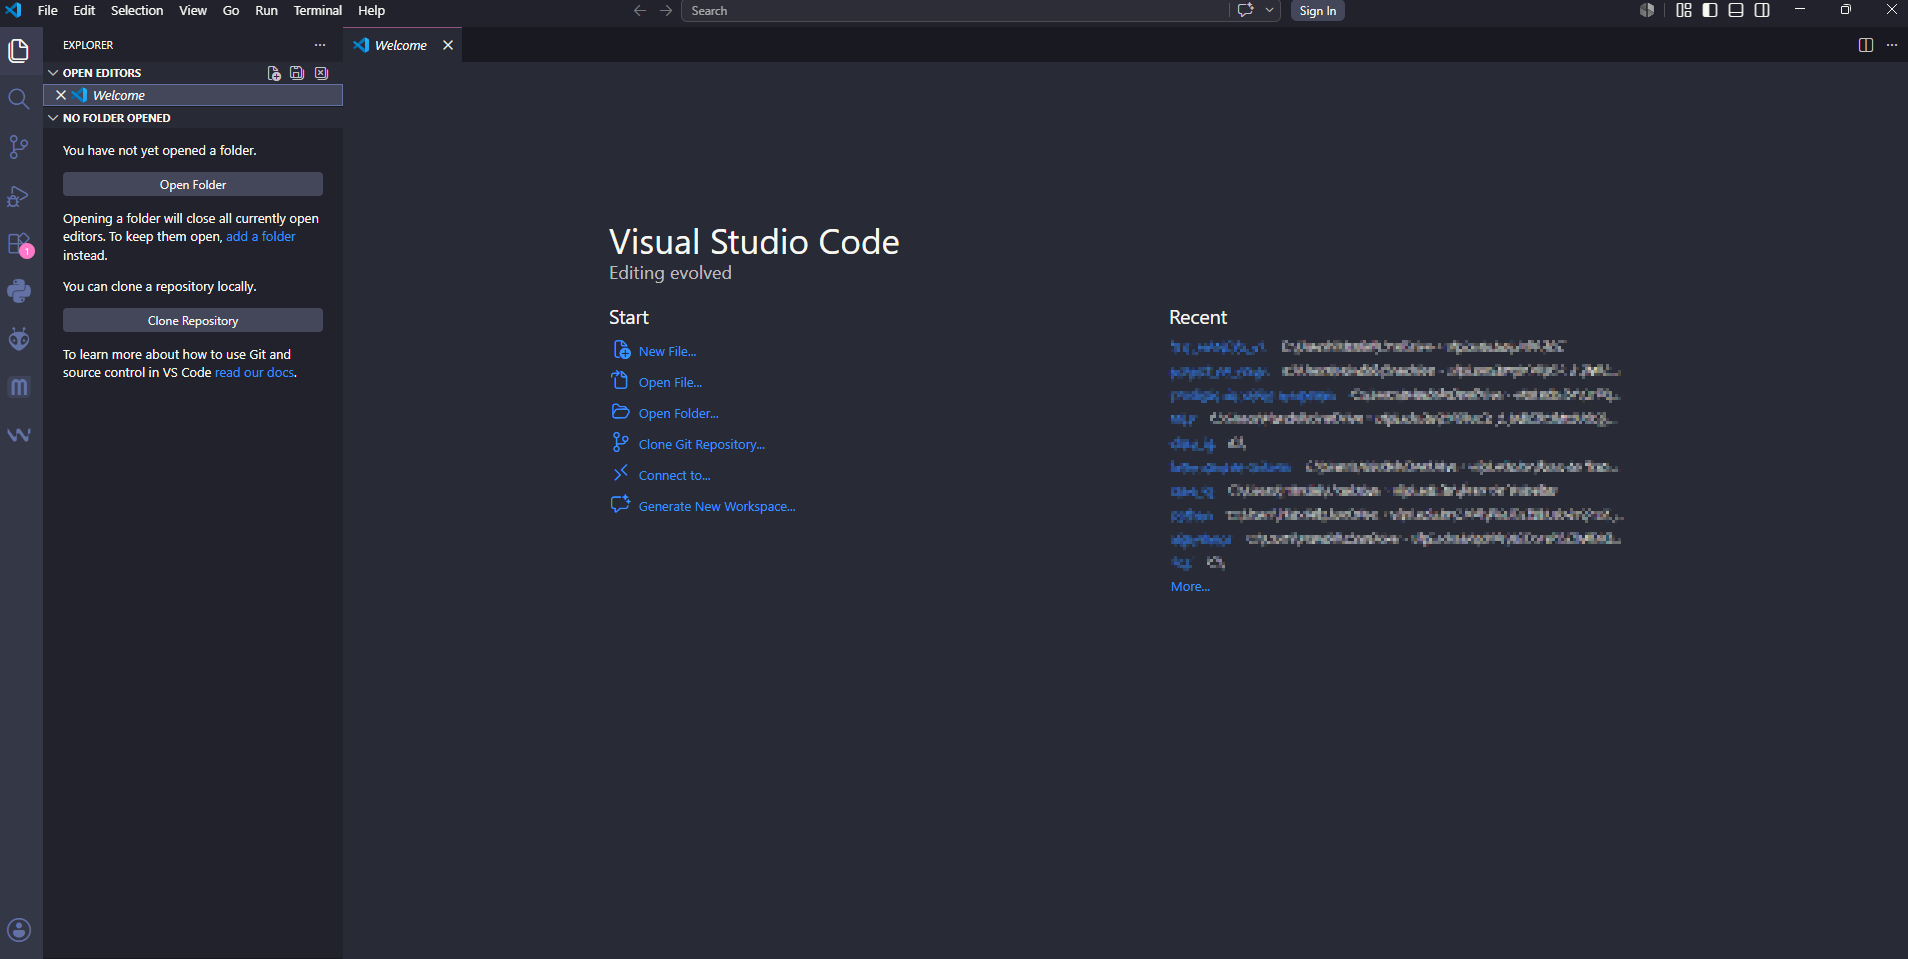
\includegraphics[width=8cm]{figuras/metodologia/interface_vscode.png}
            %     }{
            %         \Fonte{O autor}
            %     }	
            % \end{figure}

            % \begin{figure}[htbp]
            %     \centering
            %     \Caption{\label{fig:matlab-interface} Interface do MATLAB}	
            %     \UFCfig{}{
            %         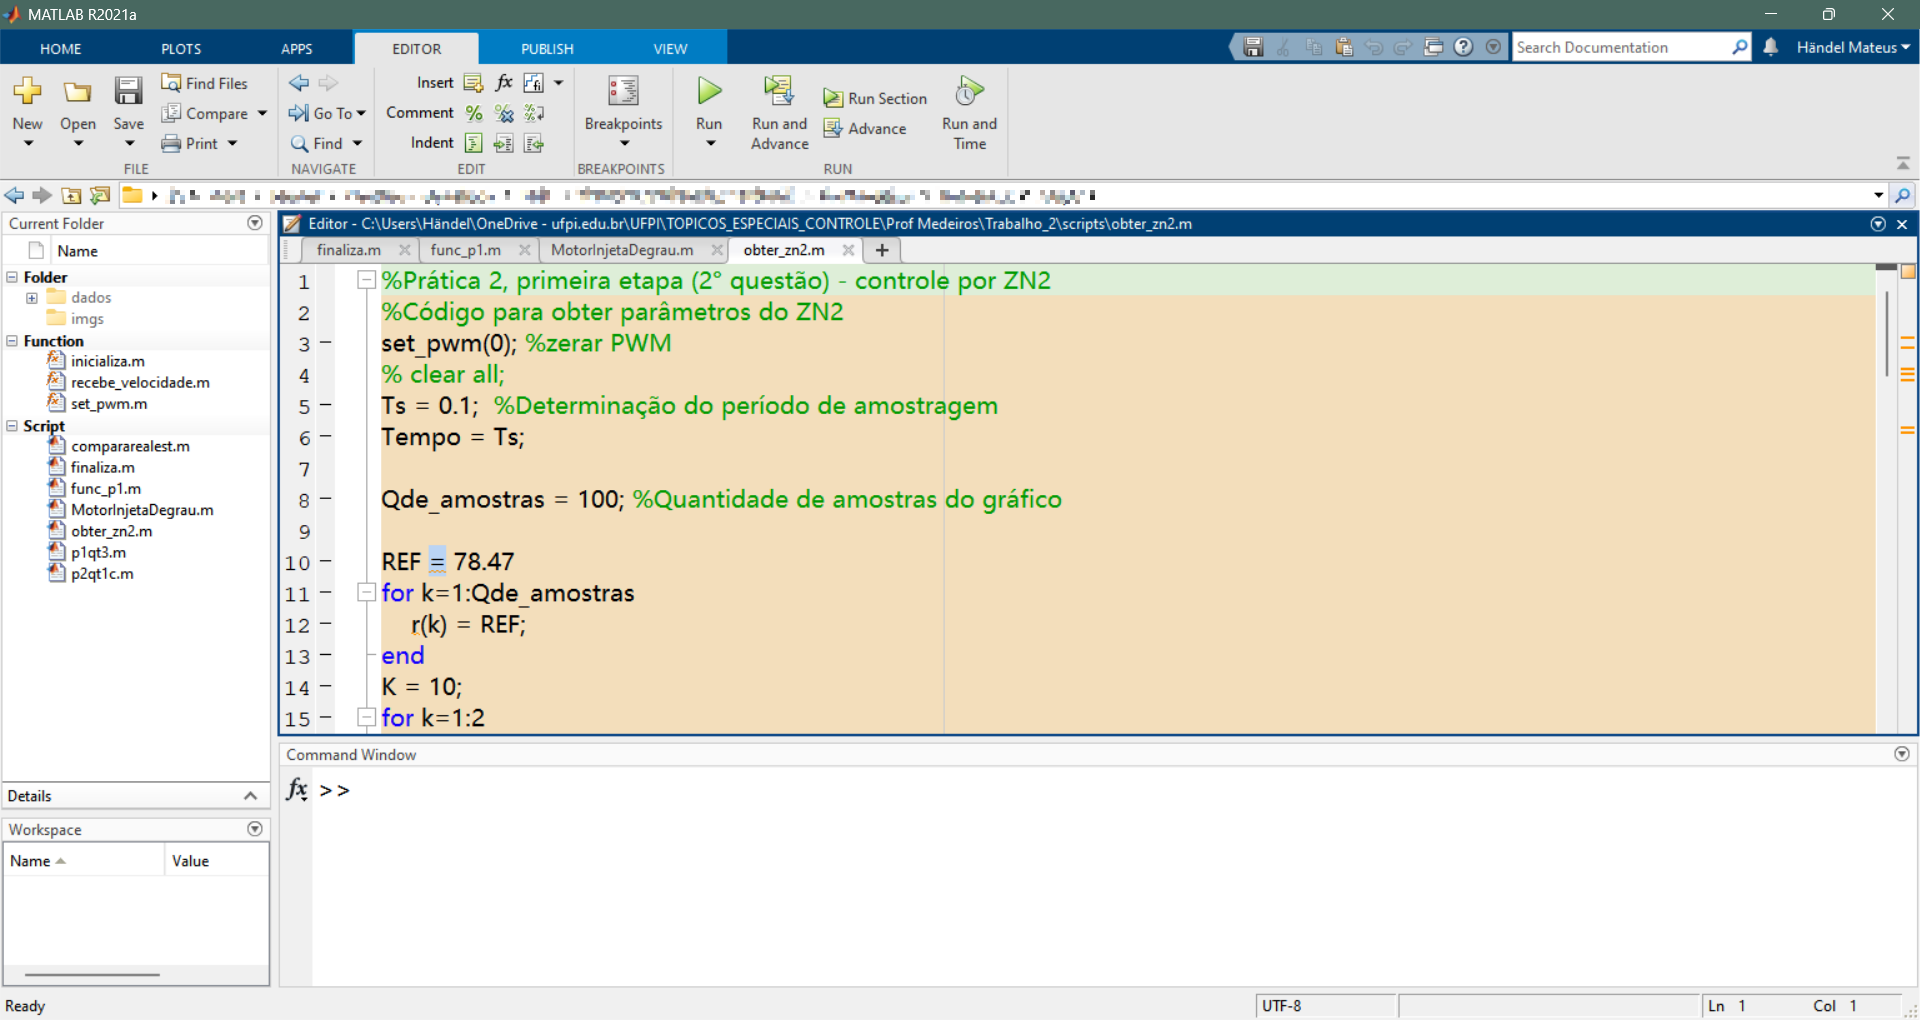
\includegraphics[width=8cm]{figuras/metodologia/interface_matlab.png}
            %     }{
            %         \Fonte{O autor}
            %     }	
            % \end{figure}

            % \begin{figure}[htbp]
            %     \centering
            %     \Caption{\label{fig:eclipse-interface} Interface do Eclipse IDE}	
            %     \UFCfig{}{
            %         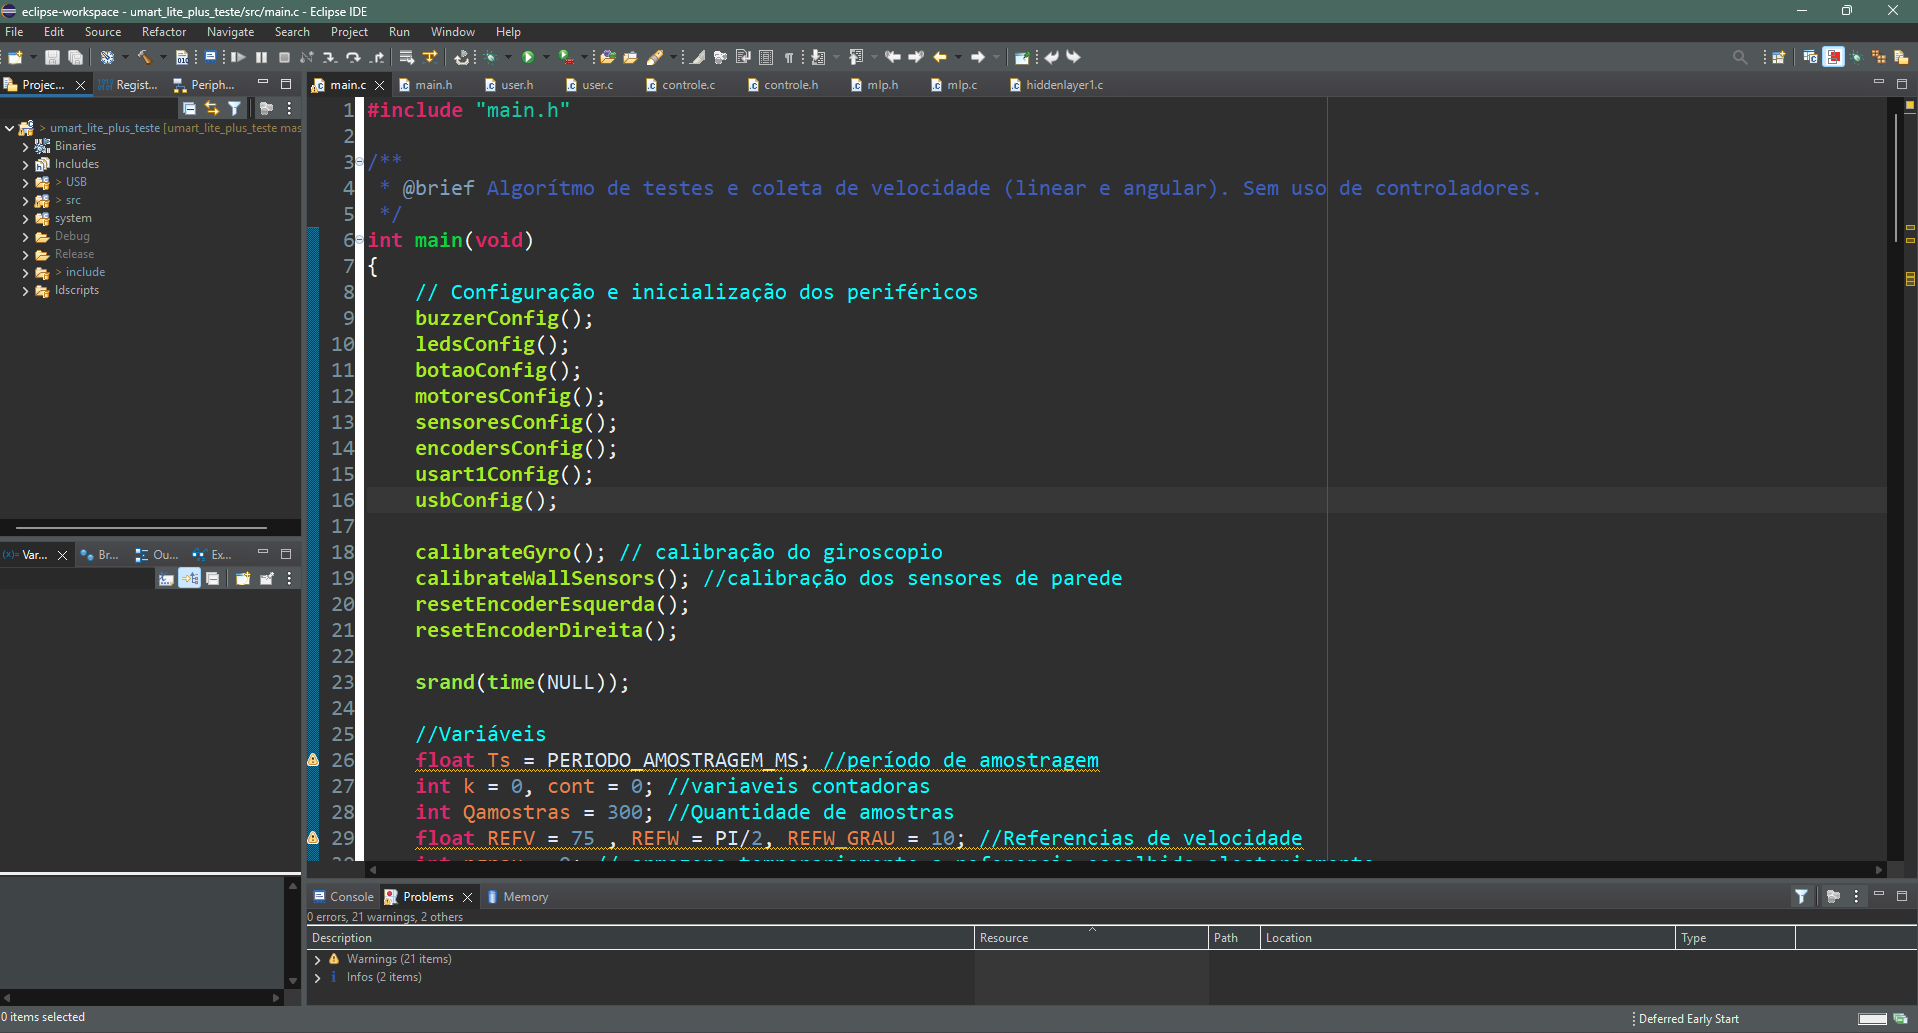
\includegraphics[width=8cm]{figuras/metodologia/interface_eclipse.png}
            %     }{
            %         \Fonte{O autor}
            %     }	
            % \end{figure}
    
    \section{Coleta de Dados} \label{sec:coleta-dados}
        Um passo necessário para realização de todo o processo de controle e monitoramento do comportamento do robô é a transferência das informações coletadas localmente para o computador. Em plantas fixas muitas vezes essa comunicação é realizada via cabo com comunicação serial, dada a sua praticidade de implementação e velocidade de transmissão. Entretanto, devido à natureza móvel da planta do presente trabalho, a necessidade muda e passa a ser a de uma comunicação que, ao menos em parte, seja sem fio. 
        
        Contudo, conforme visto em \ref{sec:caracteristicas-construtivas} o robô não dispõe de instrumentos de comunicação sem fio nativas. Por isso, inspirado no trabalho desenvolvido por \citeonline{tcc-artemio}, foi elaborada uma arquitetura de rede local de comunicação e telemetria que faz uso de dois microcontroladores do tipo ESP que trocam informações entre si via WiFi, através do protocolo ESP-NOW, sendo um do modelo ESP8266 e um ESP-WROOM-32. O ESP8266 foi escolhido devido a seu tamnho reduzido o que facilita a construção de uma estrutura para conectá-lo ao robô. O ESP-WRROM-32 foi utilizado em virtude da sua disponibilidade em laboratório. 
        
        O modelo ESP8266 está conectado ao robô e o ESP-WROOM-32 a um computador de tal modo que após a execução de um experimento a comunicação é ativada e, via serial os dados são enviados do robô para o ESP8266 e estes são transmitidos então para o ESP-WROOM-32, o qual as envia para o \gls{PC}. 
        
        As figuras \ref{fig:esp-wroom-32} e \ref{fig:esp-8266} mostram os dois microcontroladores ESP utilizados e a Figura \ref{fig:rede-comunicacao} ilustra a arquitetura descrita acima. Nesta figura o robõ encontra-se representado pelo \textit{microchip} STM32F405RGT6 apresentado à esquerda, ilustrando o seu centro de processamento dos dados.

        \begin{figure}[htbp]
            \centering
            \begin{minipage}{0.45\textwidth}
                \centering
                \Caption{\label{fig:esp-wroom-32} ESP-WROOM-32}
                %\centering
                \UFCfig{}{
                    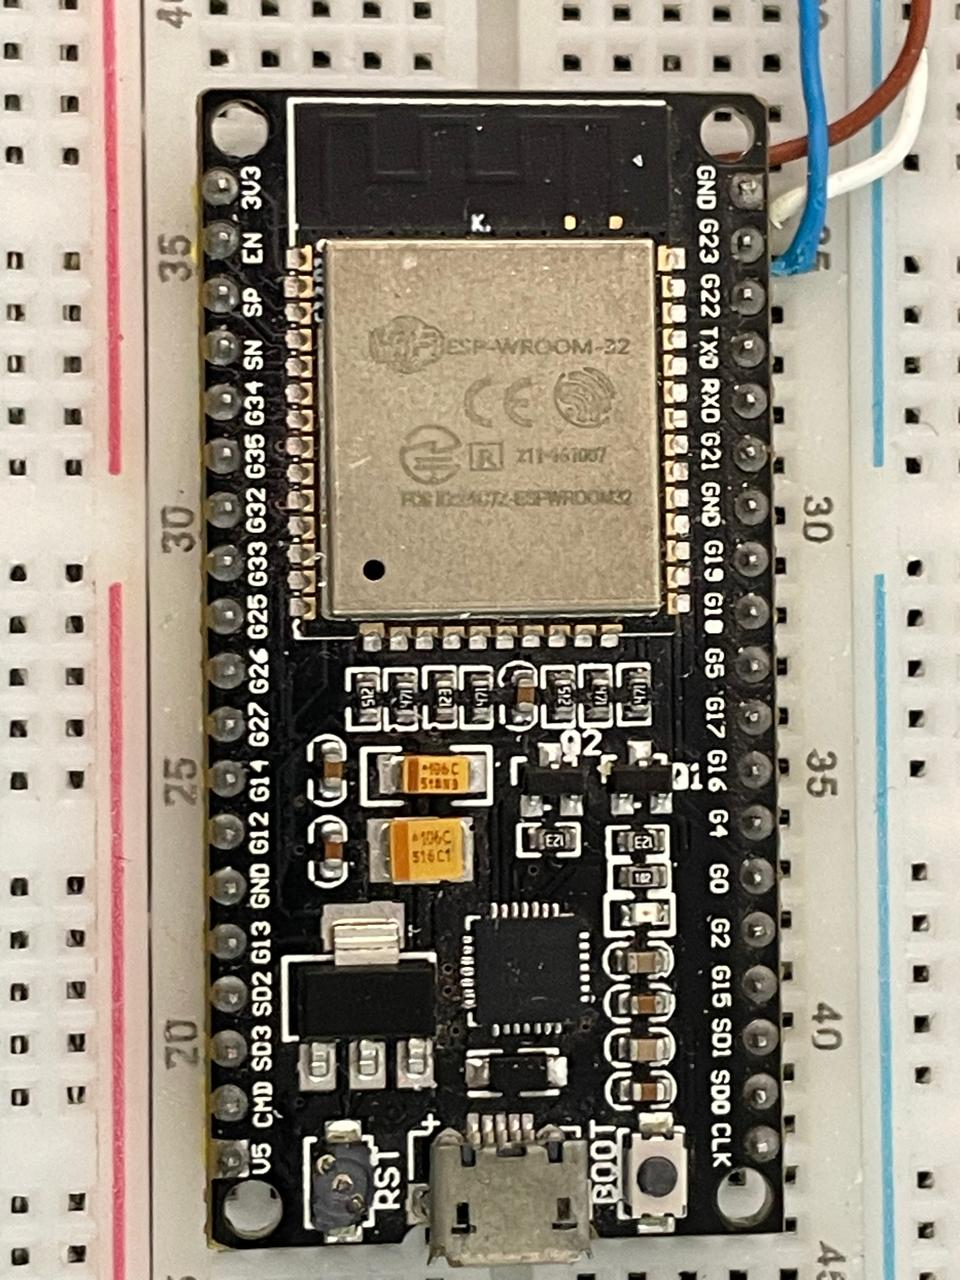
\includegraphics[width=3cm]{figuras/metodologia/esp32-wroom-32.jpg}
                }{
                    \Fonte{O autor}
                }	
            \end{minipage}
            \hfill
            \begin{minipage}{0.45\textwidth}
                \centering
                \Caption{\label{fig:esp-8266} ESP8266}
                %\centering
                \UFCfig{}{
                    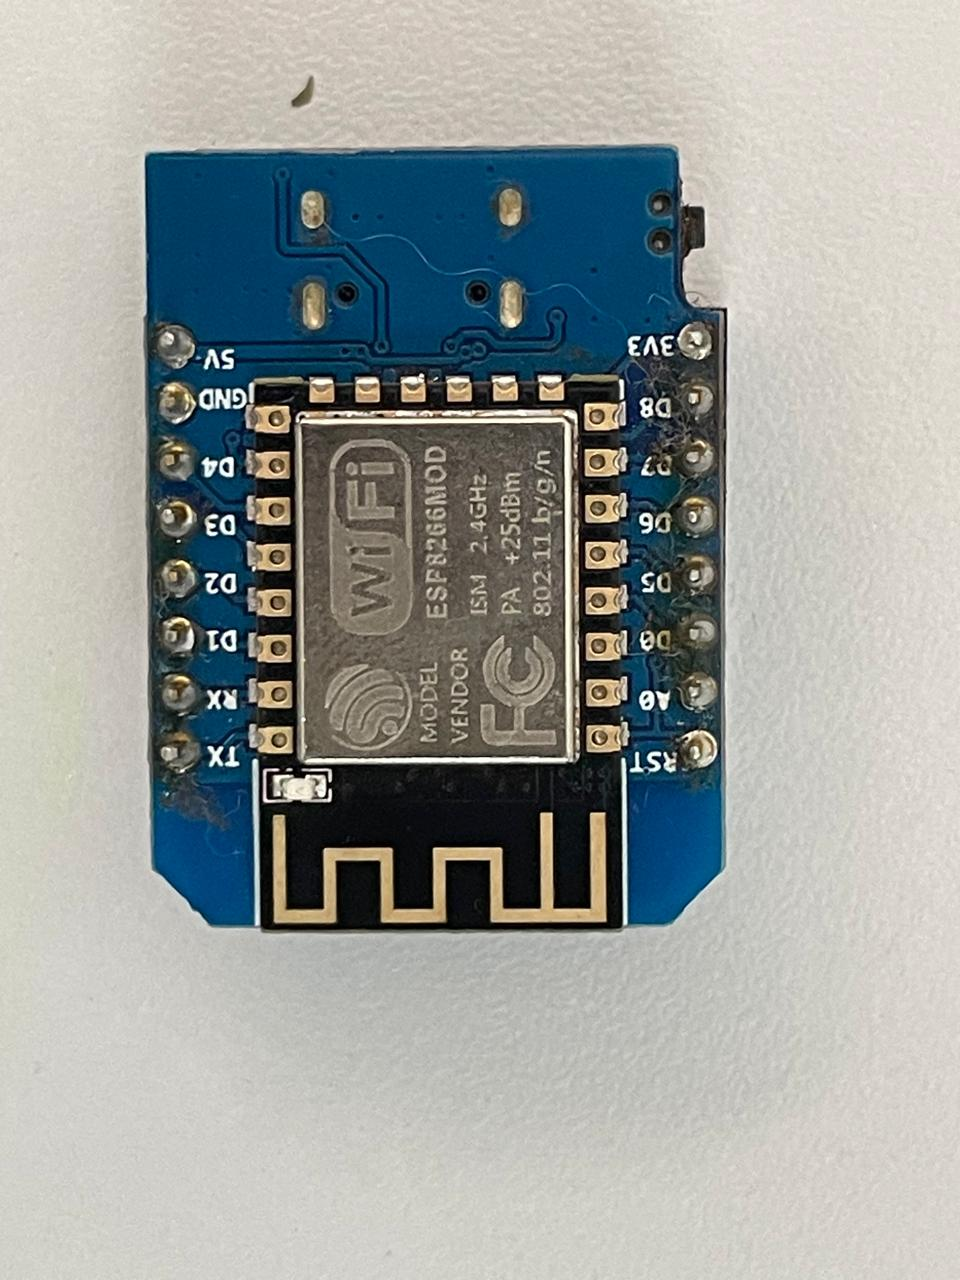
\includegraphics[width=3cm]{figuras/metodologia/esp8266-d1mini.jpg}
                }{
                    \Fonte{O autor}
                }	
            \end{minipage}
        \end{figure}

        \begin{figure}[htbp]
                \centering
                \Caption{\label{fig:rede-comunicacao} Arquitetura de rede de comunicação desenvolvida para envio de informações}	
                \UFCfig{}{
                    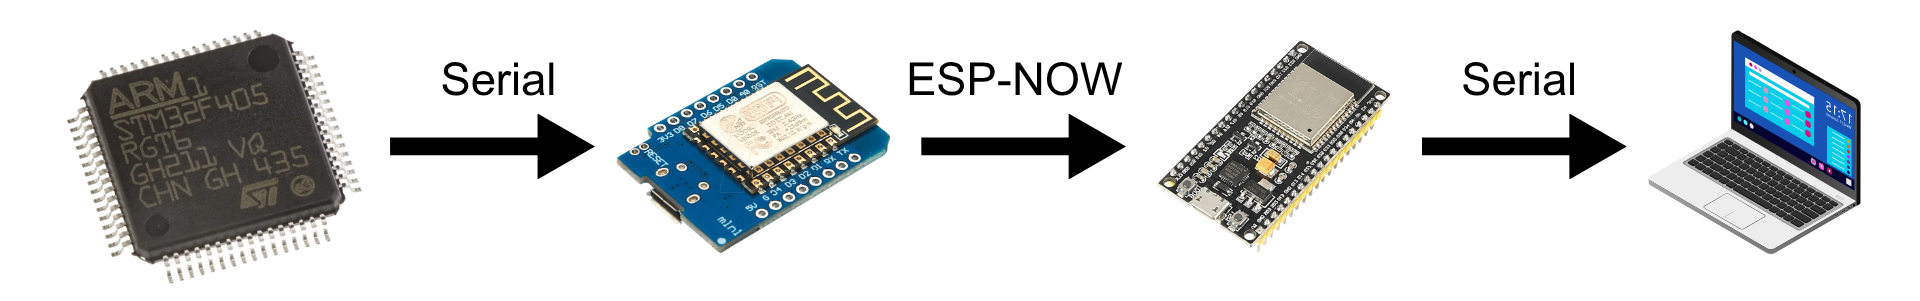
\includegraphics[width=12cm]{figuras/metodologia/rede-comunicacao-cropped.png}
                }{
                    \Fonte{O autor}
                }	
        \end{figure}

        \subsection{Comunicação e Telemetria} \label{ssec:comunicacao}
            A estrutura apresentada na Figura \ref{fig:rede-comunicacao} pode ainda ser interpretada como sendo composta por dois grupos que trocam informações via WiFi. O primeiro grupo está composto pelo STM32F405RGT6 e pelo ESP8266 e fica localizado no espaço físico do robô, onde o primeiro chip está soldado à placa e o segundo está conectado através da entrada do conector \textbf{J2} (\gls{UART}), conforme descrito em \citeonline{manual-microumouse-2015} e mostrado na Figura \ref{fig:micromouse-composicao} (aparece como “conector para módulo bluetooth”). O segundo grupo, por sua vez, é formado pelo ESP-WROOM-32 e pelo \gls{PC}, está localizado separado do robô, na bancada de trabalho, utilizando um cabo \gls{USB} para comunicação.

            \subsubsection{Comunicação Serial} \label{sssec:comunicacao-serial}
                Para a realização da comunicação no primeiro grupo foi optada pelo protocolo \gls{UART}. Nesse protocolo faz-se necessário que ambos os dispositivos possuam a mesma taxa de transferência de dados (\textit{baud rate}), haja vista a ausência de um sinal \gls{CLK} para orientar o tempo de envio dos bits. No presente trabalho foi feita a opção pela taxa de 9600 \textit{bps}, que foi a taxa que também foi adotada para o grupo contendo o ESP-WROOM-32 e o \gls{PC}.

                Para a comunicação entre o ESP-WROOM-32 e o \gls{PC} foi utilizado um cabo \gls{USB} como meio físico. Já para a comunicação entre o STM32F405RGT6 e o ESP8266 desenvolveu-se uma \gls{PCI} para ser integrada ao conector \textbf{J2} do \textit{micromouse} para realizar a conexão dos pinos de \textbf{3V3}, \textbf{GND}, \textbf{RX}, e \textbf{TX} conforme a imagem abaixo.

                \begin{figure}[htbp]
                    \centering
                    \Caption{\label{fig:conexao-stm-esp8266} Conexão de pinos entre o STM32F405RGT6 e o ESP8266}	
                    \UFCfig{}{
                        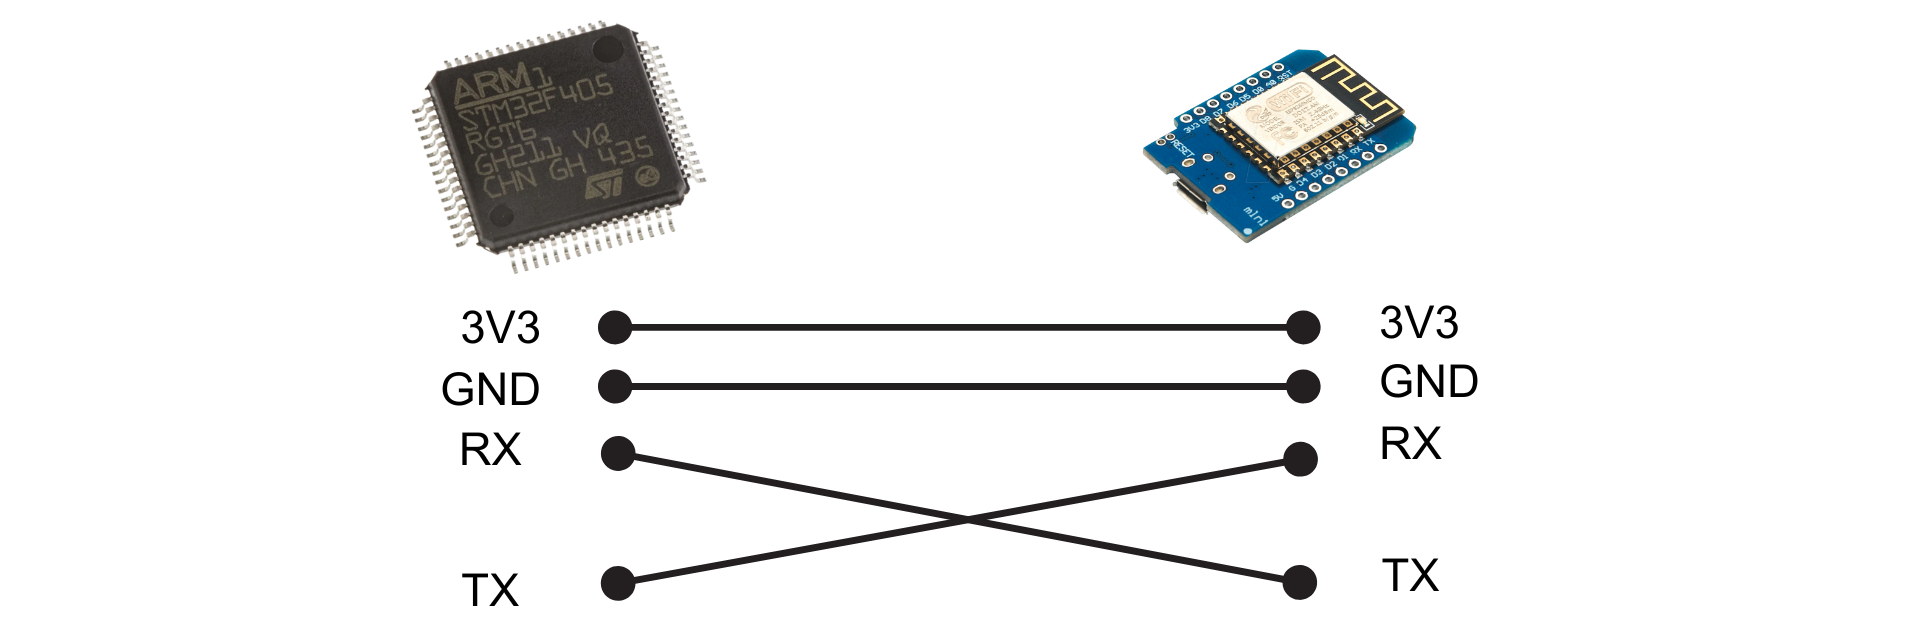
\includegraphics[width=12cm]{figuras/metodologia/uart-stm-esp8266-cropped.png}
                    }{
                        \Fonte{O autor}
                    }	
                \end{figure}

                A \gls{PCI} pode ser visualizada abaixo em seu esquemático na Figura \ref{fig:esquematico-pci} e após a sua finalização na Figura \ref{fig:pci-feita}.

                \begin{figure}[htbp]
                    \centering
                    \begin{minipage}{0.45\textwidth}
                        \centering
                        \Caption{\label{fig:esquematico-pci} Esquemático da \gls{PCI}}
                        %\centering
                        \UFCfig{}{
                            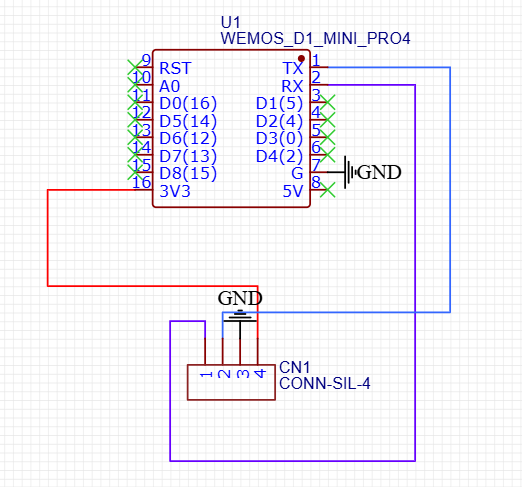
\includegraphics[width=4cm]{figuras/metodologia/esquematico_placa.png}
                        }{
                            \Fonte{O autor}
                        }	
                    \end{minipage}
                    \hfill
                    \begin{minipage}{0.45\textwidth}
                        \centering
                        \Caption{\label{fig:pci-feita} \gls{PCI} finalizada}
                        %\centering
                        \UFCfig{}{
                            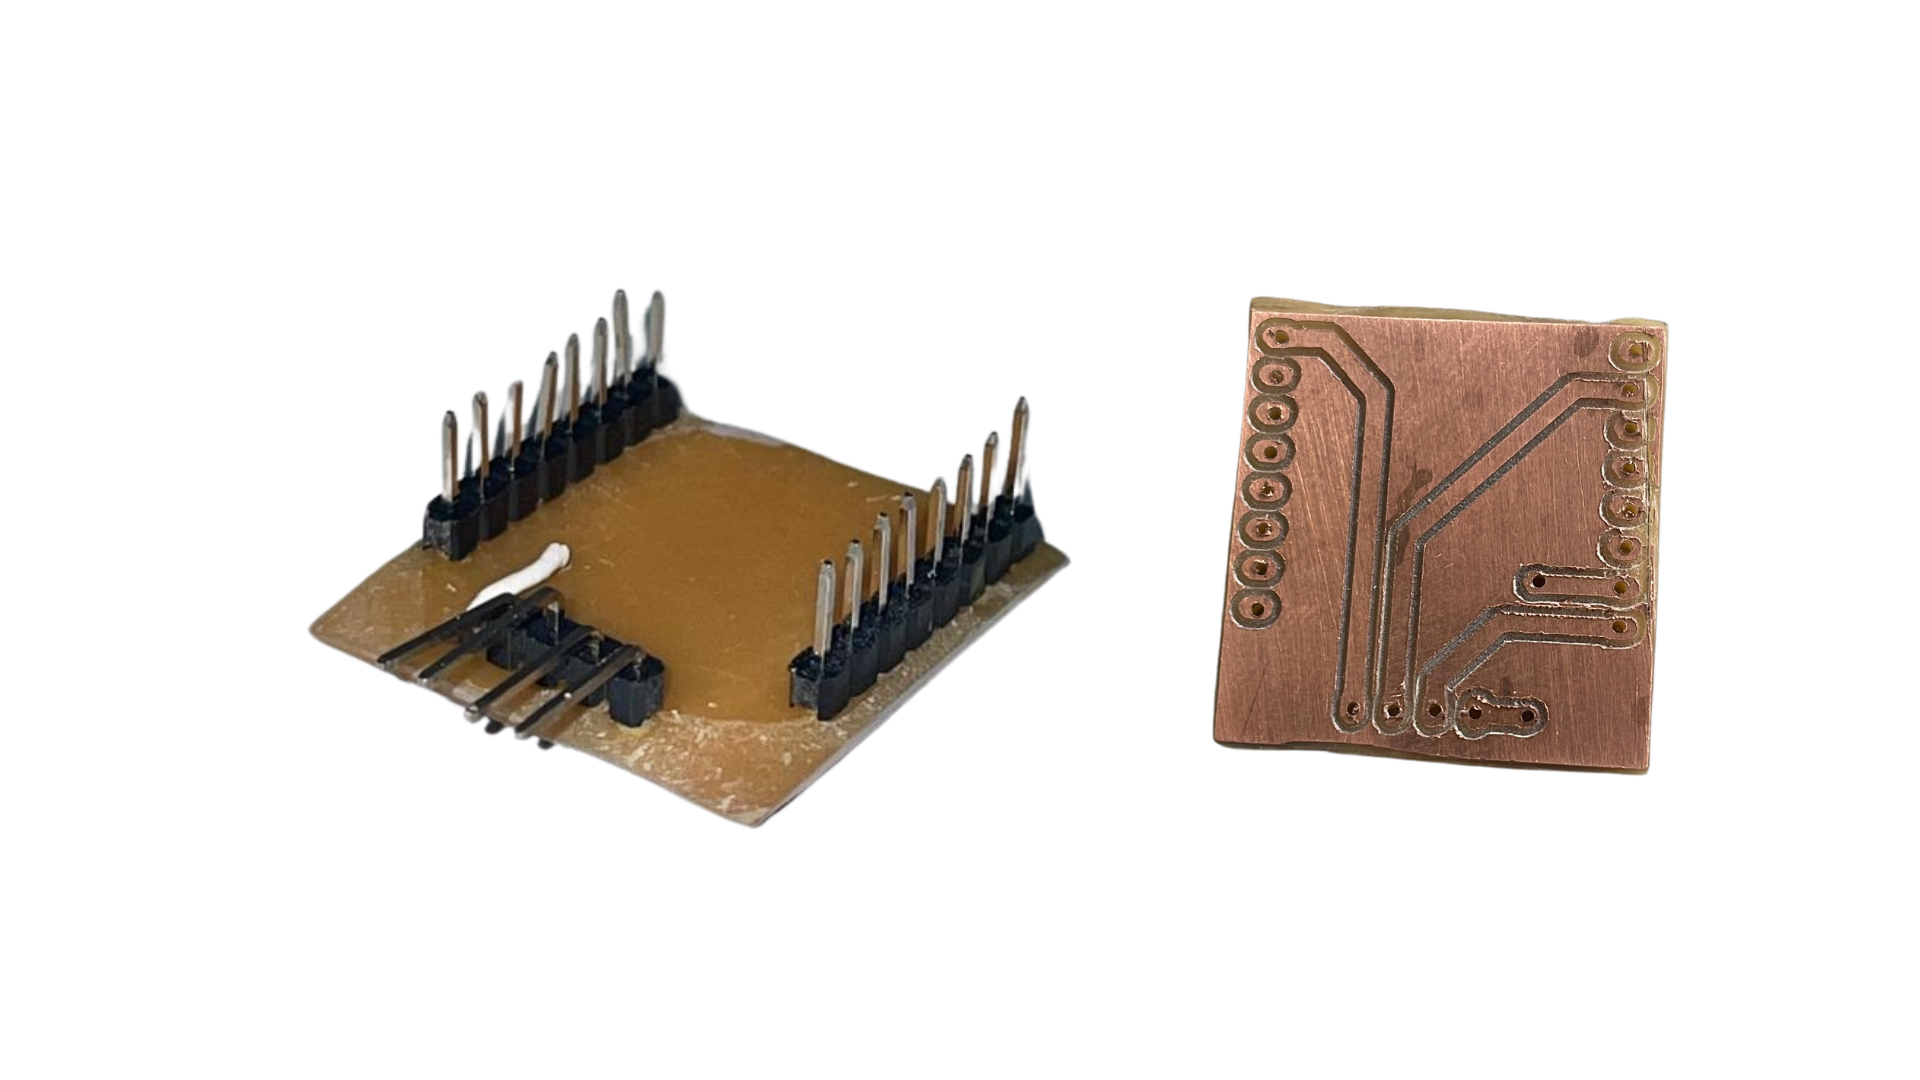
\includegraphics[width=4cm]{figuras/metodologia/placa_feita_cobre.png}
                        }{
                            \Fonte{O autor}
                        }	
                    \end{minipage}
                \end{figure}

            \subsubsection{Comunicação ESP-NOW} \label{sssec:comunicacao-esp-now}
                Conforme dito anteriormente, a comunicação sem fio se faz necessária pela natureza móvel da planta de estudo, o robô micromouse. O protocolo, desenvolvido pela \citeauthoronline{esp-now-definition},

                \begin{citacao}
                    \dots é um protocolo de comunicação sem fio baseado na camada de enlace de dados, que reduz as cinco camadas do modelo OSI para apenas uma. Assim, os dados não precisam ser transmitidos pelas camada de rede, de transporte, de sessão, de apresentação e de aplicação. Além disso, não há necessidade de cabeçalhos de pacote ou desempacotadores em cada camada, o que leva a uma resposta rápida, reduzindo o atraso causado pela perda de pacotes em redes congestionadas \cite[tradução do autor]{esp-now-definition}.
                \end{citacao}
                
                Dessa forma, o protocolo ESP-NOW se torna adequado para as necessidades de execução do projeto. Isto fica ainda mais evidenciado a partir do trabalho desenvolvido por \citeonline{tcc-artemio} o qual realizou a comparação com outros protocolos de comunicação sem fio e evidenciou a vantagem da utilização do protocolo ESP-NOW.

                No presente trabalho os dois microcontroladores ESP foram configurados tanto para enviar quanto para receber dados. Para isso, em cada um deles foi configurado da seguinte forma: 
                
                \begin{alineas}
                    \item \textit{Wifi} no modo \textbf{\textit{Wifi Station}};
                    \item Gravação do endereço MAC de destino em cada dispositivo correspondente;
                    \item Configuração \textit{Master-Slave}:
                    \begin{subalineas}
                        \item ESP8266 como \textbf{\textit{Slave}};
                        \item ESP-WROOM-32 como \textbf{\textit{Master}}.
                    \end{subalineas}
                \end{alineas}

                Essa configuração implica que apesar dos dois dispositivos poderem realizar tanto o envio quanto o recebimento de dados a comunicação é coordenada pelo ESP conectado ao \gls{PC}.  

    \section{Identificação e Controle} \label{sec:id-controle-classico-metodologia}

        De posse da estrutura desenvolvida, prosseguiu-se para a etapa de aplicações experimentais, na qual são implementados e avaliados os controladores projetados para o robô \textit{micromouse}. Essa etapa contempla os processos de \textit{Identificação} e \textit{Controle}, as quais ocorreram tanto ao nível individual -- para cada um dos motores -- quanto o nível global -- da trajetória. 
        
        Os experimentos realizados envolvem a coleta de dados e a comparação das variáveis associadas ao movimento global do robô, permitindo verificar o comportamento do sistema em condições reais de operação. Dessa forma, os experimentos realizados possibilitam analisar a resposta dos motores aos sinais de controle e avaliar o desempenho das malhas implementadas na sua capacidade de manter o robô dentro das condições de referência.

        \subsection{Identificação e Controle dos motores} \label{ssec:controle-motores}
            
            A \textit{Identificação} pode ser subdividida nas seguintes etapas. 
            
            \begin{enumerate}
                \item Coleta de dados: Medição da velocidade dos motores.
                \item Transmissão: Transferência das informações coletadas.
                \item Identificação: Aplicação de algoritmo no software MATLAB.
            \end{enumerate}
            
            O item $1$ ocorre de maneira embarcada e é coordenada pelo microcontrolador STM32F405RGT6. Já o item $2$, por sua vez, ocorre pela ação conjunta de todos os componentes da rede de comunicação. Por fim, o item $3$ é realizado utilizando apenas o \gls{PC}.

            A medição precisa da velocidade dos motores constitui a etapa fundamental para a correta identificação do sistema, uma vez que a qualidade dos modelos obtidos depende diretamente da confiabilidade dos dados experimentais coletados. Erros nessa medição comprometem a estimação dos parâmetros do modelo e, consequentemente, o desempenho das estratégias de controle projetadas a partir dele.

            Dessa forma, tomando como base as funcionalidades já disponíveis na plataforma do \textit{micromouse}, foram desenvolvidas e adaptadas rotinas computacionais destinadas à aquisição e ao processamento dos sinais provenientes dos sensores de velocidade dos motores, as quais possibilitam a obtenção das variáveis necessárias para a caracterização dinâmica do sistema e para as etapas subsequentes de identificação e projeto de controladores. 

            Após a implementação das rotinas de medição, realizou-se a normalização dos sinais de entrada e saída dos motores, mapeando-os para o intervalo entre $0\%$ e $100\%$ a fim de padronizar a escala das variáveis manipuladas e medidas, facilitando a análise dos dados experimentais, a identificação dos modelos e o projeto dos controladores. 
            
            A utilização de variáveis normalizadas contribui para a uniformização das grandezas envolvidas nas etapas de controle em \gls{MA} e \gls{MF}, reduzindo problemas decorrentes de diferenças de escala entre sinais e simplificando a interpretação dos resultados obtidos.
        
            Na fase de comunicação, o STM32F405RGT6 envia dados ao ESP8266 via \gls{UART}, que os repassa ao ESP-WROOM-32, armazenando-os em estruturas separadas para cada motor. Posteriormente, os dados são transferidos ao \gls{PC} via \gls{USB}, onde o MATLAB solicita informações sobre o tipo de dado e o motor ao qual ele se refere. Assim, com os dados coletados, é possível analisar a resposta do sistema a diferentes entradas, como degrau, rampa ou sinais randomizados.
        
            Baseado em \citeonline{tcc-marcolino} e usando como resposta a entrada a um degrau, para determinação do período de amostragem dos motores, foi determinado um período de amostragem de $T_s = 10ms$. Além disso, aplicou-se então uma entrada randomizada em torno de um degrau de referência, oscilando entre $\pm 10\%$ desse mesmo degrau, e coletou-se a saída para cada um dos motores. A partir dos dados coletados é possível, então, aplicar o algoritmo do estimador \gls{MQNR} e, assim, prosseguir com a identificação e com o desenvolvimento dos controladores.
            
            O projeto dos controladores foi realizado segundo a autossintonia baseada no Método do Relé, descrita na Seção \ref{sec:autossintonia-rele}. Inicialmente, foram implementados controladores \gls{PID} para o controle individual da velocidade de cada roda do robô, conforme ilustrado na Figura \ref{fig:controle-motores-individuais}. Essa abordagem permite atuar diretamente sobre a dinâmica de cada motor, proporcionando melhor rastreamento de referência e reduzindo os efeitos de diferenças entre ambos os motores.

            \begin{figure}[htb]
                \centering
                \Caption{\label{fig:controle-motores-individuais} Controle dos Motores Individuais}	
                    \UFCfig{}{
                        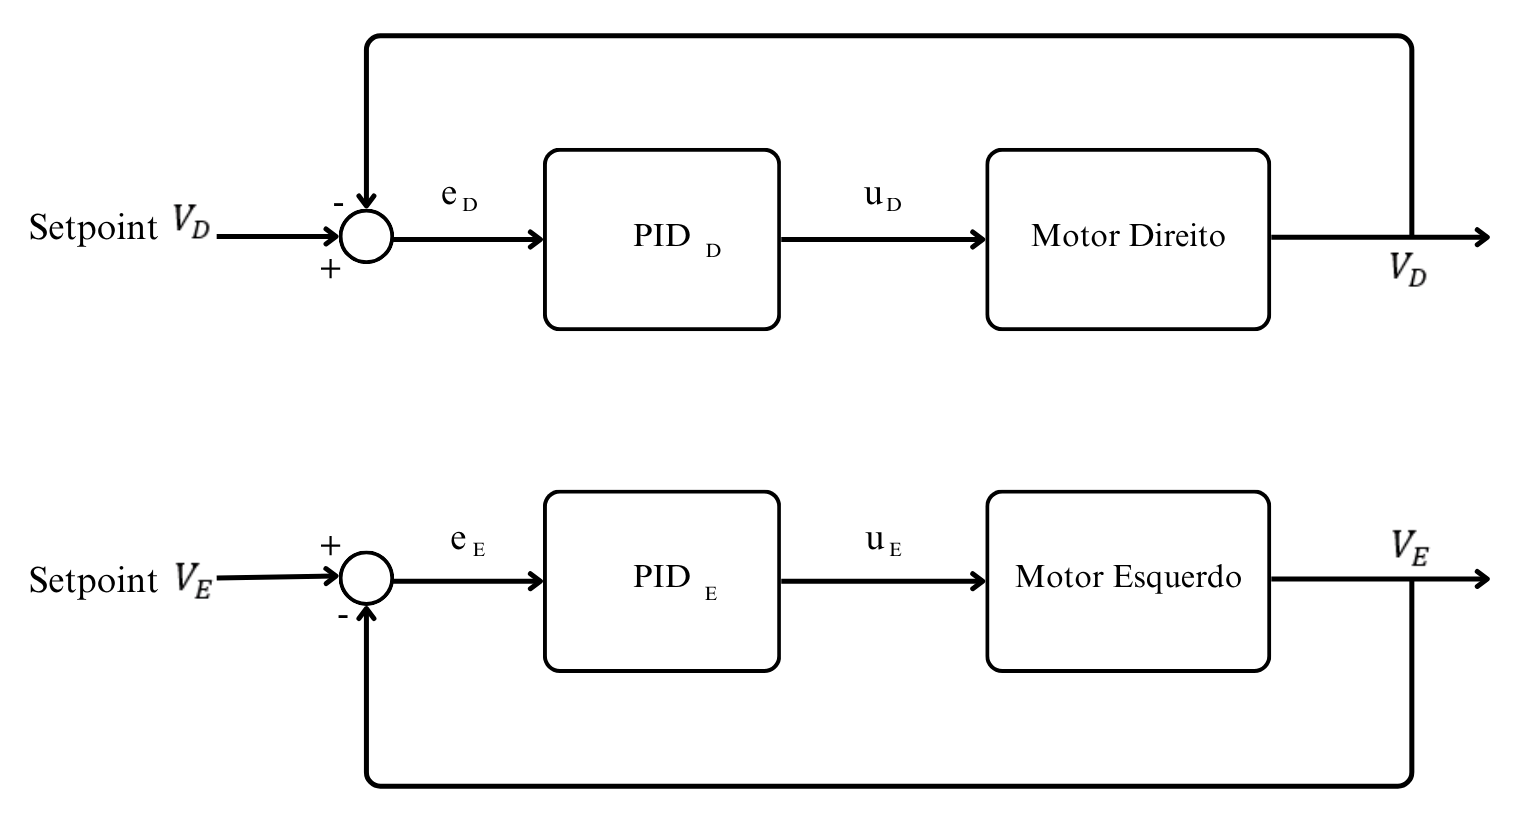
\includegraphics[width=9cm]{figuras/metodologia/malha-controle-motor-individual.png}
                    }{
                        \Fonte{O autor}
                    }	
            \end{figure}

        \subsection{Identificação e Controle das variáveis globais} \label{ssec:controle-trajetoria}

            Com os controladores individuais aplicados procedeu-se com a identificação e controle das variáveis globais de movimento do \textit{micromouse}, responsáveis pelo adequado seguimento de trajetória. A \textit{Identificação} seguiu os mesmos procedimentos apresentados anteriormente. Após isso, foram implementadas as duas malhas de controle de nível superior, denominadas como malhas \textit{supervisórias}, responsáveis pela geração dos \textit{setpoints} aplicados aos controladores individuais. 
            
            Conforme a Figura \ref{fig:controle-malhas-globais}, essas malhas atuam sobre as variáveis globais de movimento do robô, coordenando a ação dos controladores das rodas de modo a controlar o comportamento cinemático do \textit{micromouse} de forma integrada.        

            \begin{figure}[htb]
                \centering
                \Caption{\label{fig:controle-malhas-globais} Controle Supervisório Incluso}	
                    \UFCfig{}{
                        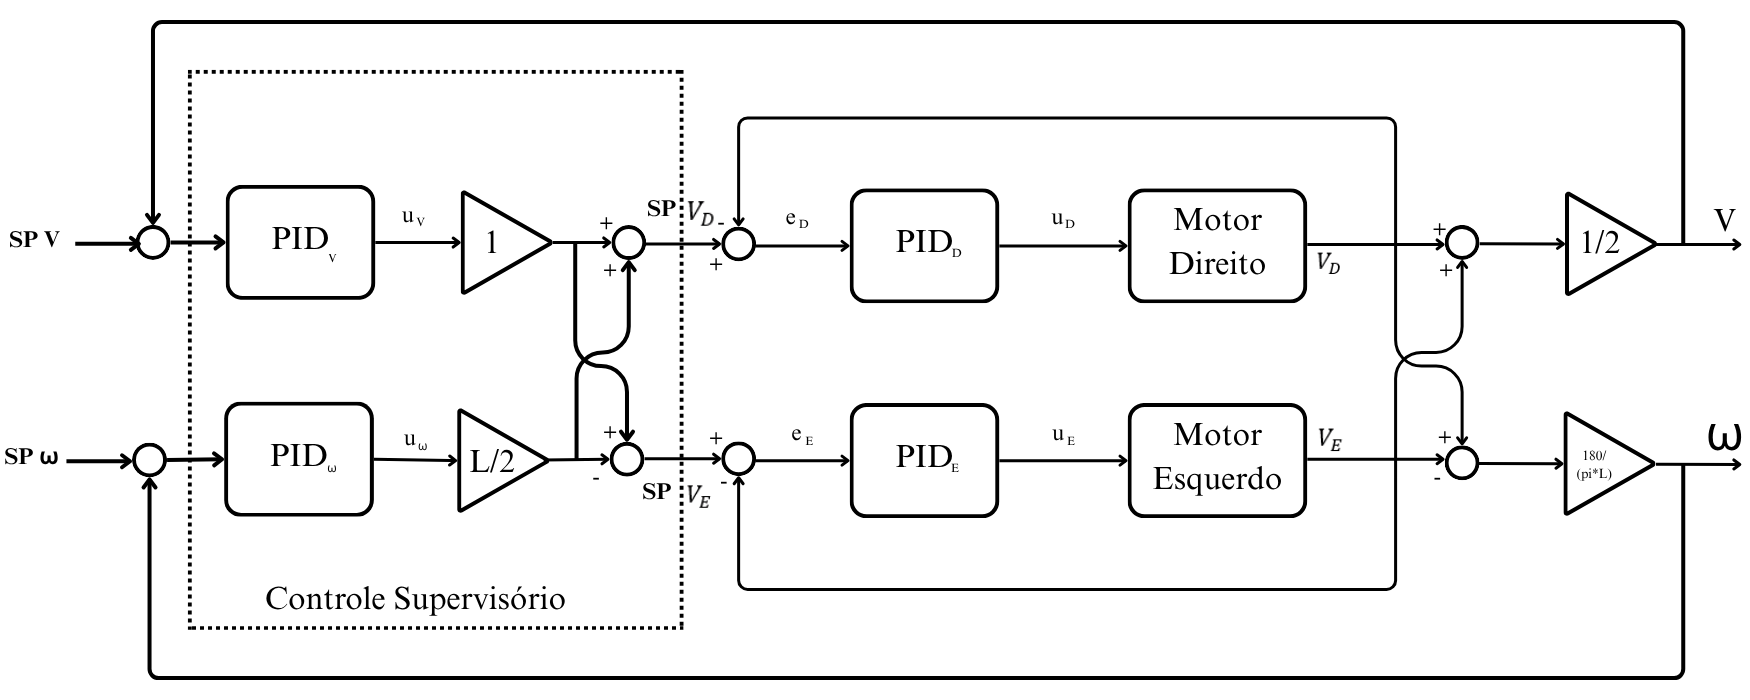
\includegraphics[width=16cm]{figuras/metodologia/malha-controle-global.png}
                    }{
                        \Fonte{O autor}
                    }	
            \end{figure}
            
            A partir da Figura \ref{fig:controle-malhas-globais} observa-se, também, a inclusão de dois somadores e de blocos multiplicadores após os blocos \textit{Motor Direito} e \textit{Motor Esquerdo} cuja função é a representação das relações cinemáticas do robô.

            Vale ressaltar ainda que projeto dos controladores $PID_V$ e $PID_\omega$ foi realizado também desconsiderando as interações entre as malhas de $V$ e $\omega$, ou seja, os sistemas foram considerados como sendo \gls{SISO} o que facilita o projeto quando comparado ao desenvolvimento de controladores \gls{MIMO}. Isto se deu tendo em vista que os controladores individuais dos motores apresentam, também, a função de desacoplamento entre essas malhas superiores conforme explicitado em \citeonline{dissetacao-pereira-2000}.
            
            Assim, após a obtenção dos ganhos dos controladores \gls{PID} destinados tanto aos motores quanto às variáveis globais de movimento, esses parâmetros são gravados no robô seguindo o apresentado na Seção \ref{ssec:programacao-e-bootloader} para a execução dos experimentos práticos. Com isso, conclui-se a etapa de projeto e implementação das estratégias de controle, estabelecendo-se a base necessária para a validação experimental do sistema. 
            
            % No capítulo \ref{cap:resultados}, a seguir, são apresentados os resultados obtidos bem como as respectivas análises, considerações e interpretações.


            % \begin{citacao}
            %     Quando existem controladores de velocidade locais devidamente ajustados e suficientemente rápidos para terem suas dinâmicas desprezadas, a relação estática entre os sinais de controle e o seu efeito é sempre constante. Como os controladores têm ainda as mesmas características, além de constantes estes ganhos são iguais. $[\dots]$. Com isto, prova-se que uma outra função para os controladores locais de velocidade é o desacoplamento entre os controladores de orientação e posição.
            % \end{citacao}
            
              
	\chapter{Resultados} \label{cap:resultados}

    Nesta seção serão apresentados e discutidos os resultados obtidos do desenvolvimento do trabalho tendo como base a fundamentação apresentada nos capítulos \ref{cap:id-e-controle} e \ref{cap:micromouse} e da metodologia desenvolvida no Capítuo \ref{cap:metodologia}. 
    
    Conforme será visto e detalhado nas seções a seguir, primeiro foram trabalhadas as malhas de controle internas, isto é, dos motores, realizando a devida identificação e controle, que se encontram apresentados na Seção \ref{sec:res-motores}. Posteriormente, foram trabalhadas as malhas das variáveis globais de controle cujos resultados estão apresentados na Seção \ref{sec:res-global}.

    \section{Testes realizados nos motores} \label{sec:res-motores}
        
        Inicialmente, para determinação da identificação dos motores é necessária a correta amostragem do processo dos motores. Assim, tendo como base testes experimentais e os resultados apresentados em \citeonline{tcc-marcolino}, o período de amostragem foi definido como sendo $T_s = 10ms$.

        De posse disso é produzido um sinal \gls{PRBS} em torno de um valor central de referência $R$ usando um valor de margem $\varDelta x = 0.1R$. Este sinal é empregado em identificação de sistemas por apresentar características semelhantes às de um ruído aleatório sendo, entretanto, determinístico e reprodutível. Dessa forma, é possível excitar o sistema em uma ampla faixa de frequências, permitindo evidenciar sua dinâmica.
        
        % O sinal é construído usando um registrador de deslocamento \gls{LFSR} dentro do microcontrolador juntamente da operação lógica \textit{XOR}. A regra que define a saída do \gls{PRBS} é apresentado na Equação \ref{eq:deslocamento-bit}. A saída possui dois níveis lógicos de forma que se $b(k) = 1$ a resposta produz um sinal $R + \varDelta x$, e se $b(k) = 0$ é produzido um sinal $R - \varDelta x$, o que pode ser definido pela Equação \ref{eq:saida-prbs}.

        Neste trabalho, o sinal é gerado por meio de um registrador de deslocamento com realimentação linear -- \gls{LFSR} -- implementado no microcontrolador. A sequência binária é produzida a partir da operação lógica \textit{XOR} entre posições específicas do registrador. Embora a sequência gerada seja periódica, seu período é suficientemente elevado para que, durante os experimentos, apresente comportamento semelhante ao de um sinal aleatório.

        A saída do \gls{PRBS} possui dois níveis lógicos. Quando $b(k)=1$, o sinal de entrada assume o valor $R+\varDelta x$, enquanto para $b(k)=0$ a entrada passa a assumir o valor $R-\varDelta x$. A regra de geração da sequência binária é apresentada na Equação \ref{eq:deslocamento-bit}, enquanto a definição do sinal aplicado ao sistema é dada pela Equação~\ref{eq:saida-prbs}.

        \begin{equation}
            \label{eq:deslocamento-bit}
            b(k) = s_{15}(k)\oplus s_{14}(k)
        \end{equation}

        \begin{equation}
            \label{eq:saida-prbs}
            u(k) = 
            \begin{cases}
                R + \varDelta x, & b(k) = 1 \\
                R - \varDelta x, & b(k) = 0
            \end{cases}
        \end{equation}
        
        \subsection{Identificação dos motores} \label{sec:res-id-motores}

            Assim, um sinal \gls{PRBS} com $R = 50\%$ é aplicado a cada um dos motores e suas resposta são coletadas e apresentadas nas Figuras \ref{fig:saida-prbs-motor-direito} e \ref{fig:saida-prbs-motor-esquerdo}. Nestas figuras estão apresentados o sinal de entrada, em vermelho, aplicado aos motores e o sinal de resposta de cada um deles, na cor preta.  
            
            \begin{figure}[htb]
                \centering
                \Caption{\label{fig:saida-prbs-motor-direito} Resposta do motor direito}	
                    \UFCfig{}{
                        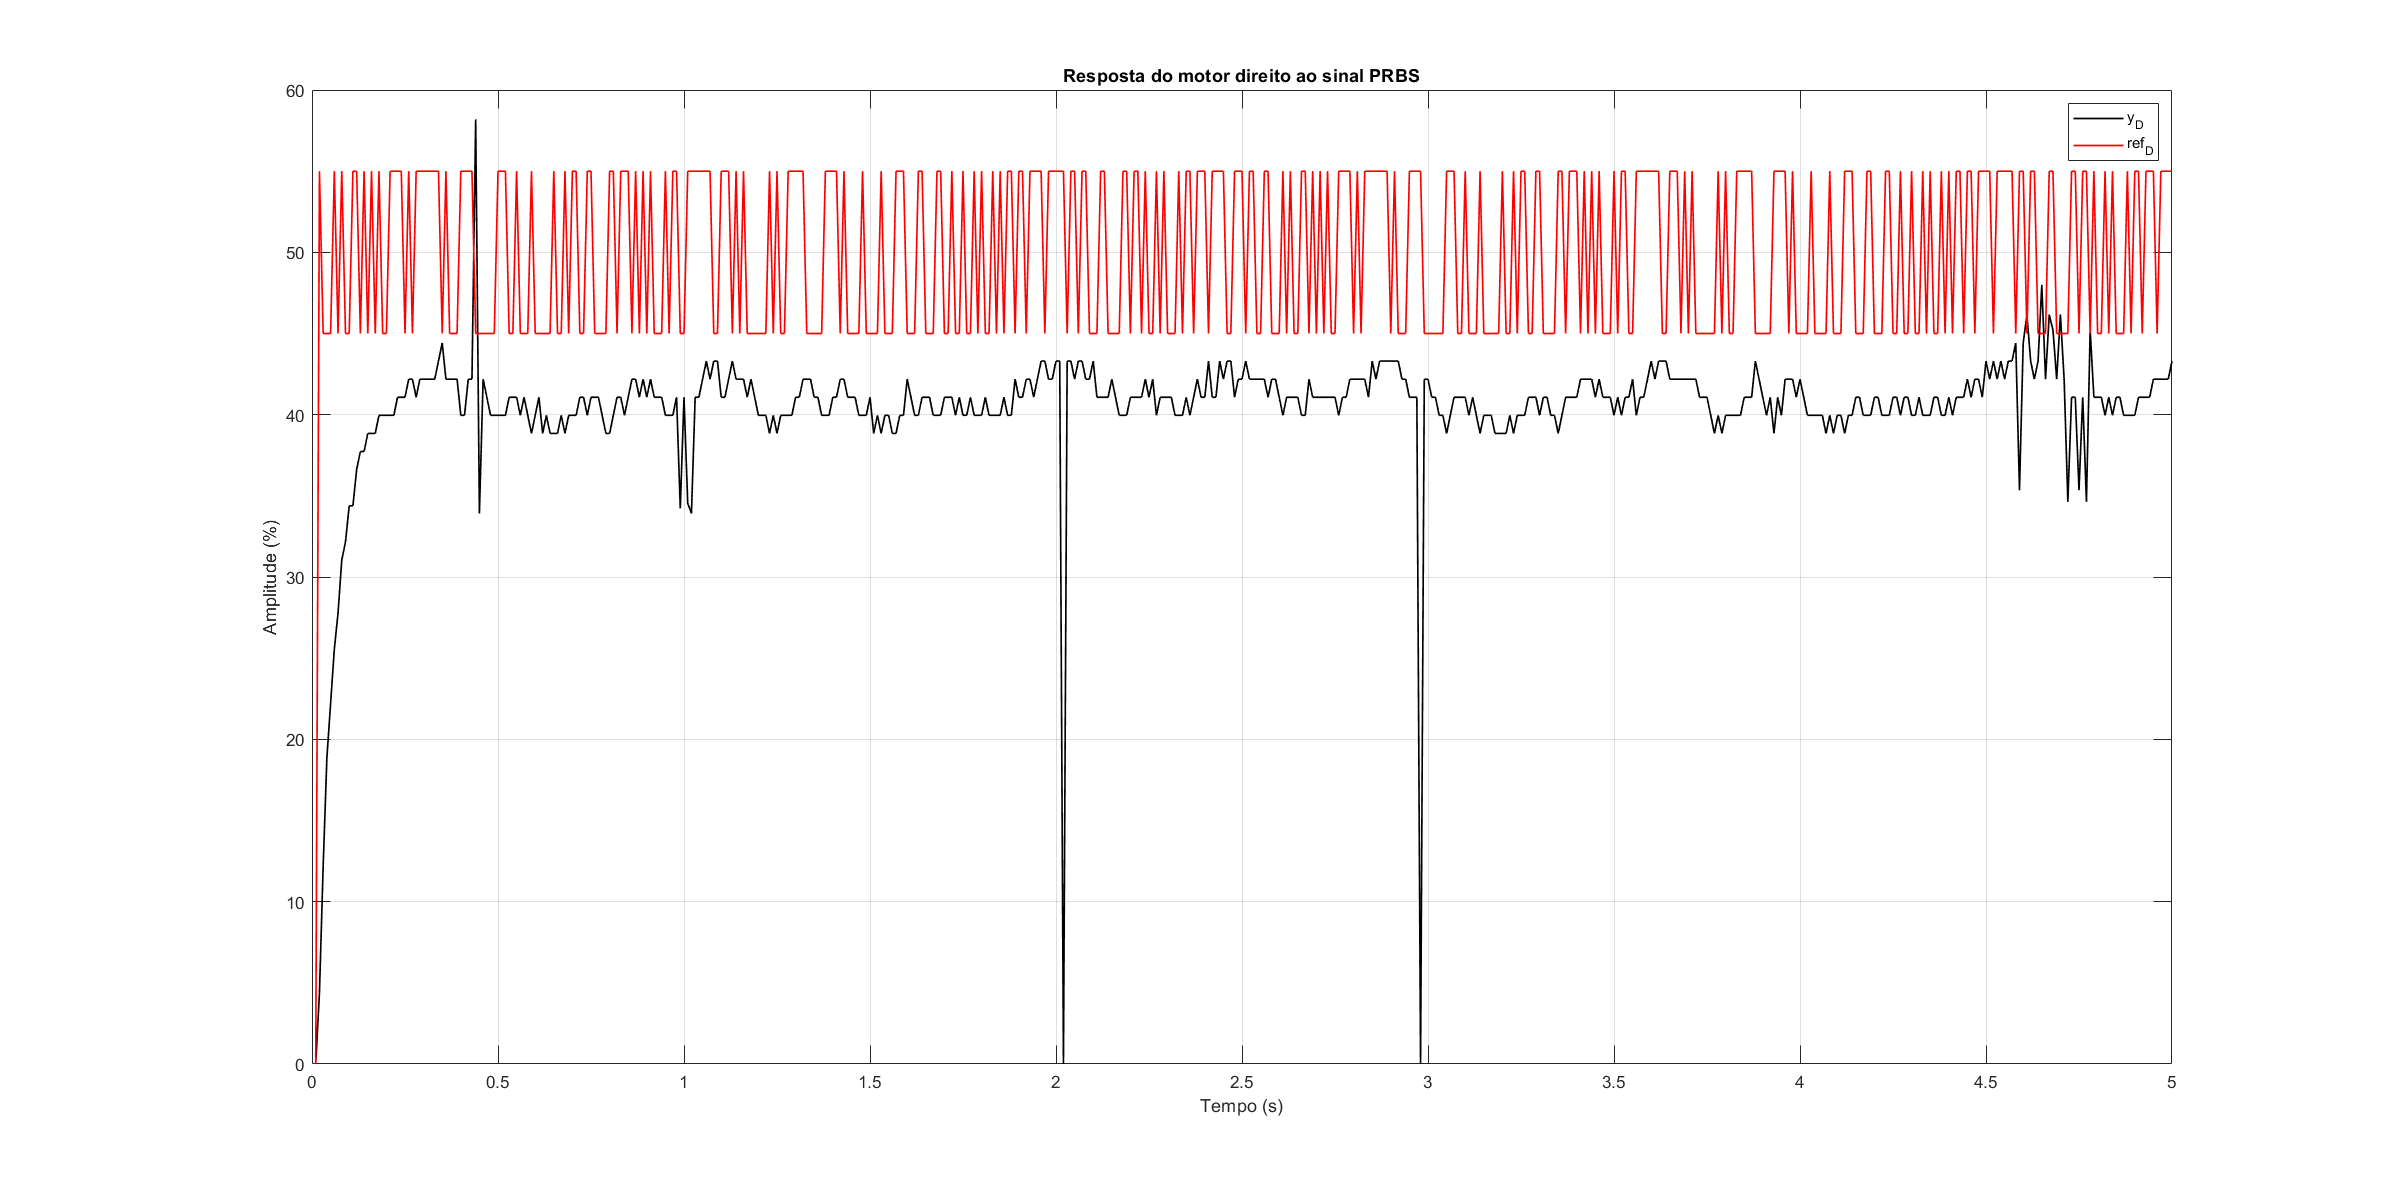
\includegraphics[width=16cm]{figuras/resultados/fig-motores/resp_mot_dir_prbs.png}
                    }{
                        \Fonte{O autor}
                    }	
            \end{figure}

            \begin{figure}[htb]
                \centering
                \Caption{\label{fig:saida-prbs-motor-esquerdo} Resposta do motor esquerdo}	
                    \UFCfig{}{
                        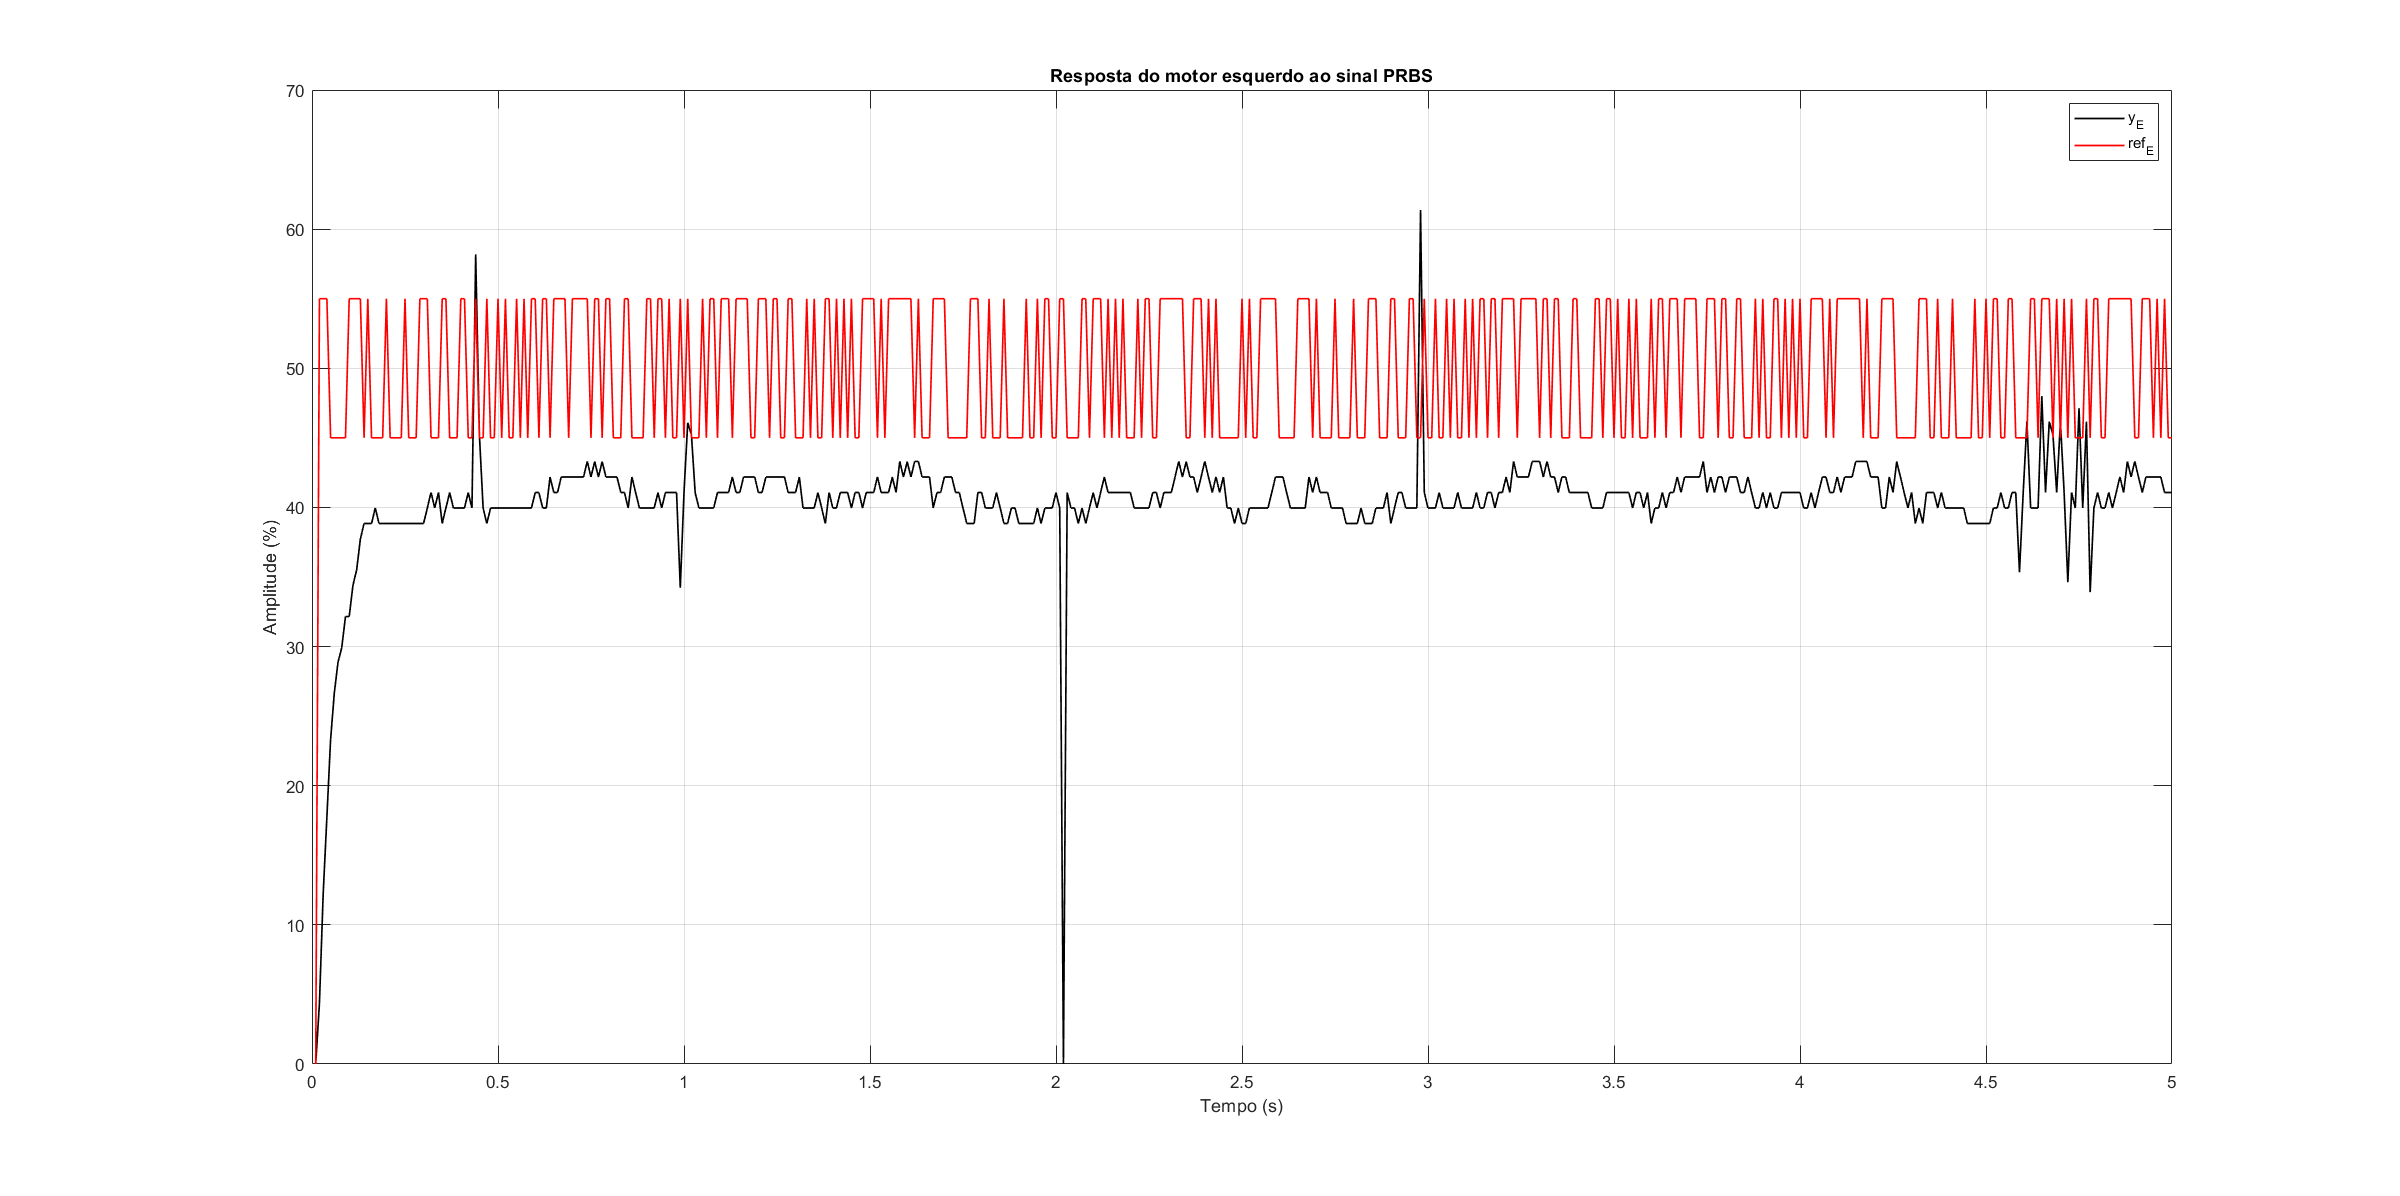
\includegraphics[width=16cm]{figuras/resultados/fig-motores/resp_mot_esq_prbs.png}
                    }{
                        \Fonte{O autor}
                    }	
            \end{figure}
            
            Com os dados coletados é possível então a aplicação do método \gls{MQNR} para identificação e construção dos modelos metamáticos de cada um dos motores conforme a Equação \ref{eq:ft-ordem-2-z-com-atraso}. Os resultados usados para validas as respectivas identificações são apresentados nas Figuras \ref{fig:identificacao-motor-direito} e \ref{fig:identificacao-motor-esquerdo}. Em cada uma das figuras estão contidos dois \textit{plots}, onde o superior contém, em preto, o sinal de resposta do motor, também apresentado nas figuras anteriores, e, em vermelho, o sinal obtido da aplicação dos modelos obtidos. Já no segundo \textit{plot}, em azul, está apresentado o sinal de erro de identificação, correspondendo à diferença entre a saída real e a saída modelada.

            \begin{figure}[ht]
                \centering
                \Caption{\label{fig:identificacao-motor-direito} Identificação do motor direito}	
                    \UFCfig{}{
                        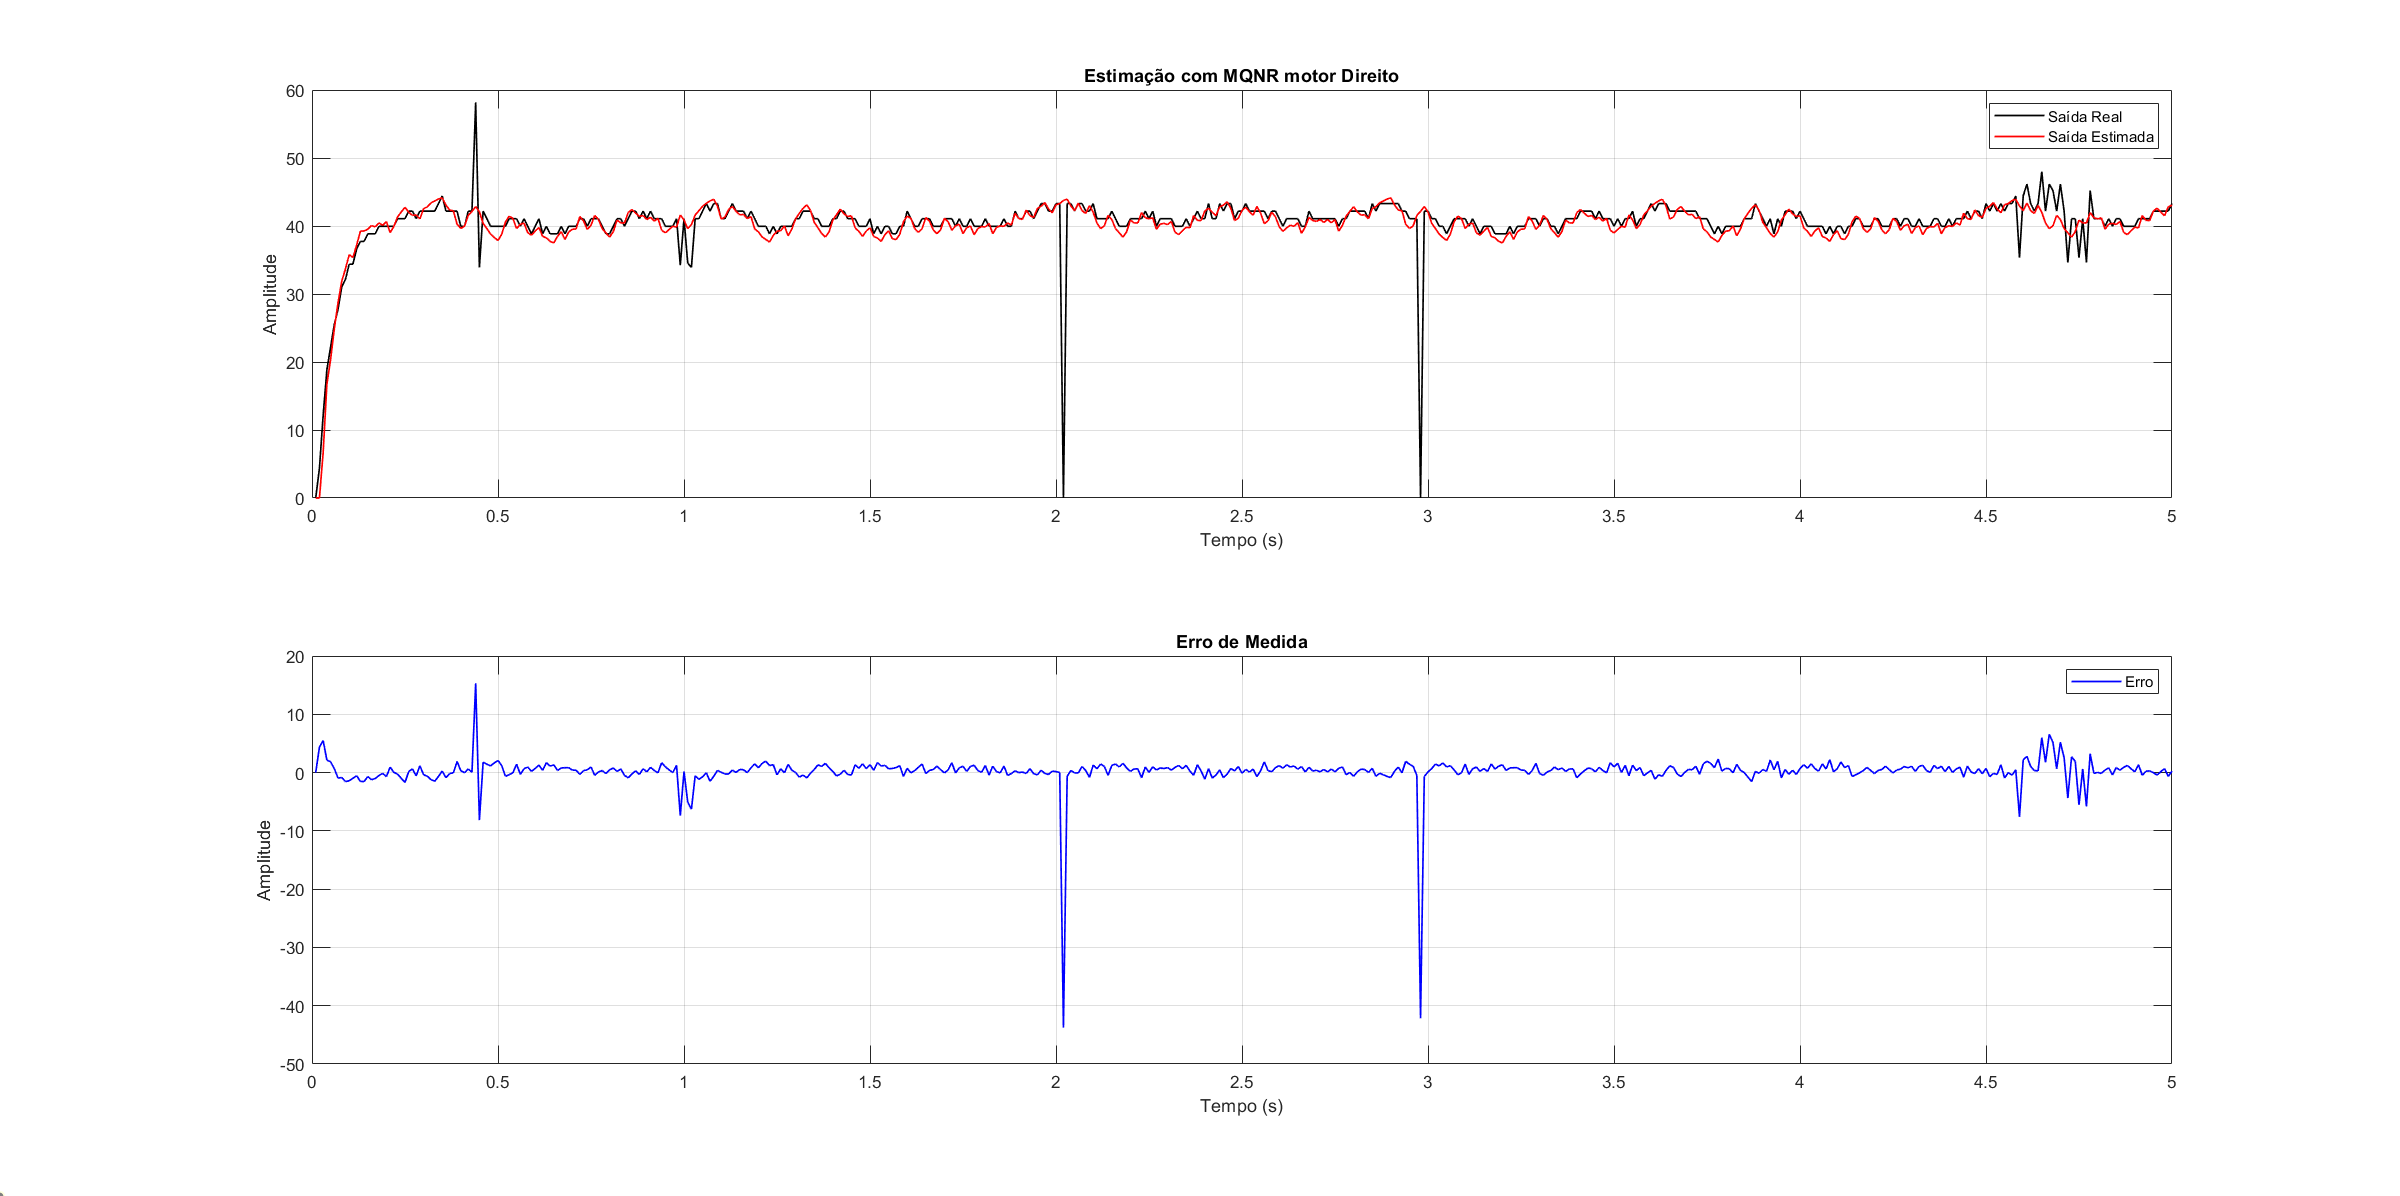
\includegraphics[width=16cm]{figuras/resultados/fig-motores/identifica_motor_direito.png}
                    }{
                        \Fonte{O autor}
                    }	
            \end{figure}

            \begin{figure}[ht]
                \centering
                \Caption{\label{fig:identificacao-motor-esquerdo} Identificação do motor esquerdo}	
                    \UFCfig{}{
                        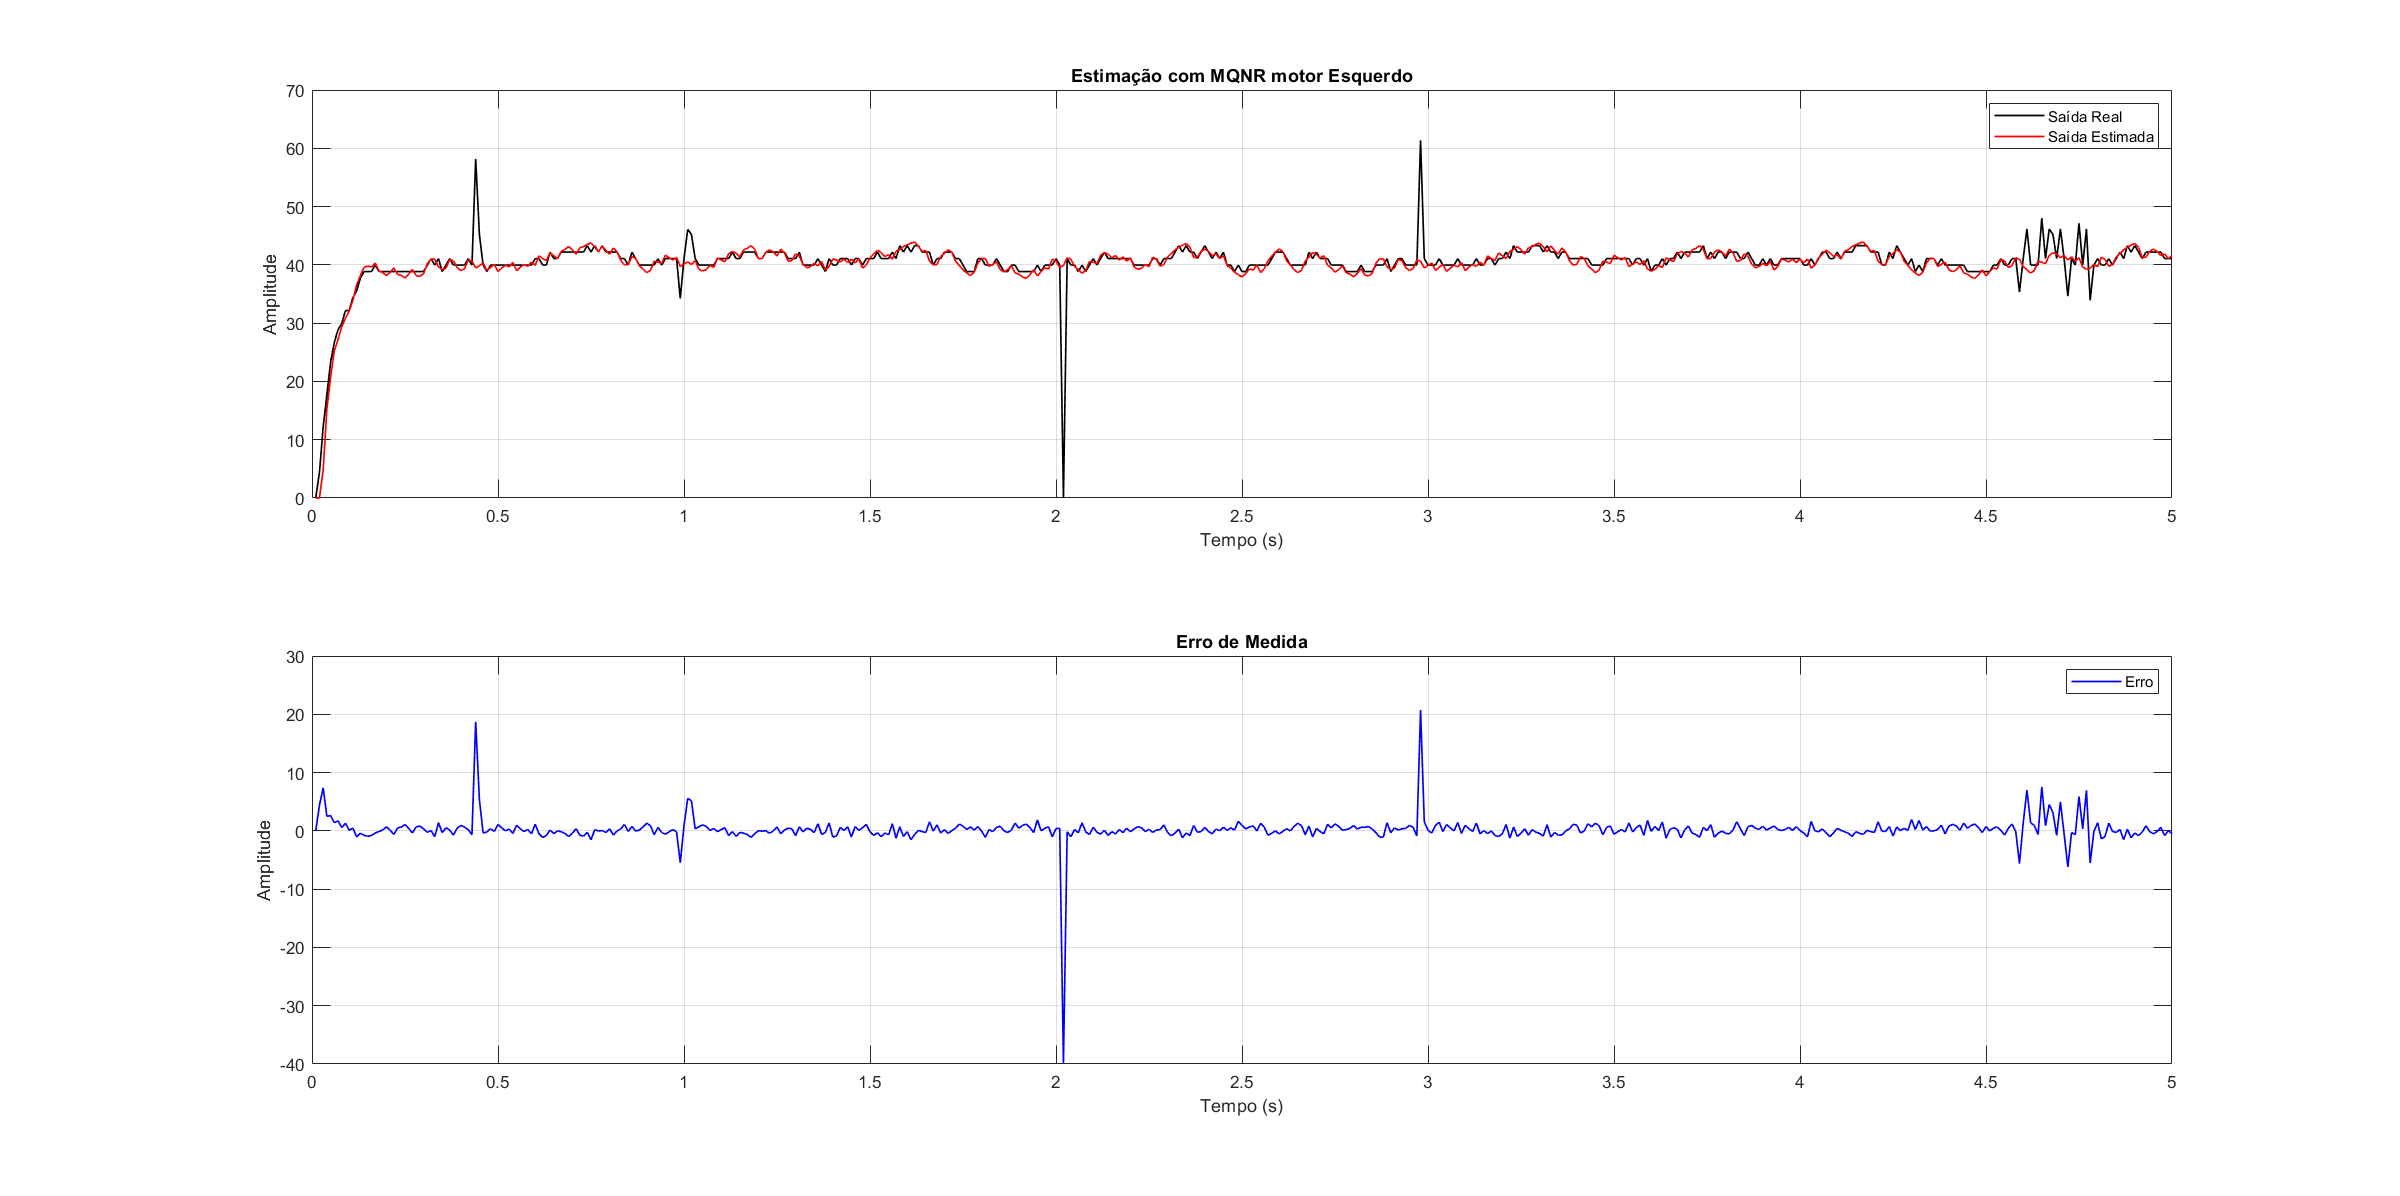
\includegraphics[width=16cm]{figuras/resultados/fig-motores/identifica_motor_esquerdo.png}
                    }{
                        \Fonte{O autor}
                    }	
            \end{figure}

            É possível observar que, para ambos os casos, o método aplicado obtém uma resposta que pode ser considerada satisfatória, haja vista que o gráfico do erro de identificação encontra-se próximo de zero, com exceção dos pontos de ruído de medição os quais não são representados pelo modelo, fazendo com que, nesses pontos, o erro seja maior. Os coeficientes obtidos da identificação de cada um dos motores são apresentados a seguir na Tabela \ref{tab:identificacao-motores}.

            \begin{table}[!htbp]	
				\centering
				\Caption{\label{tab:identificacao-motores} Coeficientes dos modelos dos motores}
				\UFCtab{}{
					\begin{tabular}{ccc}
						\toprule
						Coeficiente/Motor & \( Direito \) & \( Esquerdo \) \\
						\midrule
						\( a_1 \) & \( -0.3101 \) & \( -0.2496 \) \\
						\( a_2 \)    & \( -0.3252 \) & \( -0.3680 \) \\
						\( b_1 \)   & \( 0.1326 \) & \( 0.1281 \) \\
                        \( b_2 \)   & \( 0.1651 \) & \( 0.1821 \) \\
						\bottomrule
					\end{tabular}
				}{
					\Fonte{O autor}
				}
			\end{table}

        \subsection{Controle aplicado nos motores} \label{sec:res-controle-motores}

            Com os modelos em mãos, é possível prosseguir para a etapa de projeto dos controladores a partir do método do Relé. Os resultados da aplicação de um relé em cada um dos modelos dos motores são apresentados nas Figuras \ref{fig:rele-modelo-direito} e \ref{fig:rele-modelo-esquerdo} e os parâmetros utilizados são apresentados na Tabela \ref{tab:parametros-rele-motores}. Em cada uma das Figuras \ref{fig:rele-modelo-direito} e \ref{fig:rele-modelo-esquerdo} é possível observar três sinais: o sinal de referência, em verde, o sinal de entrada do Relé, em preto, e o sinal da resposta do sistema modelado ao Relé, em vermelho.
            
            \begin{figure}[ht]
                \centering
                \Caption{\label{fig:rele-modelo-direito} Relé no modelo do motor direito}	
                    \UFCfig{}{
                        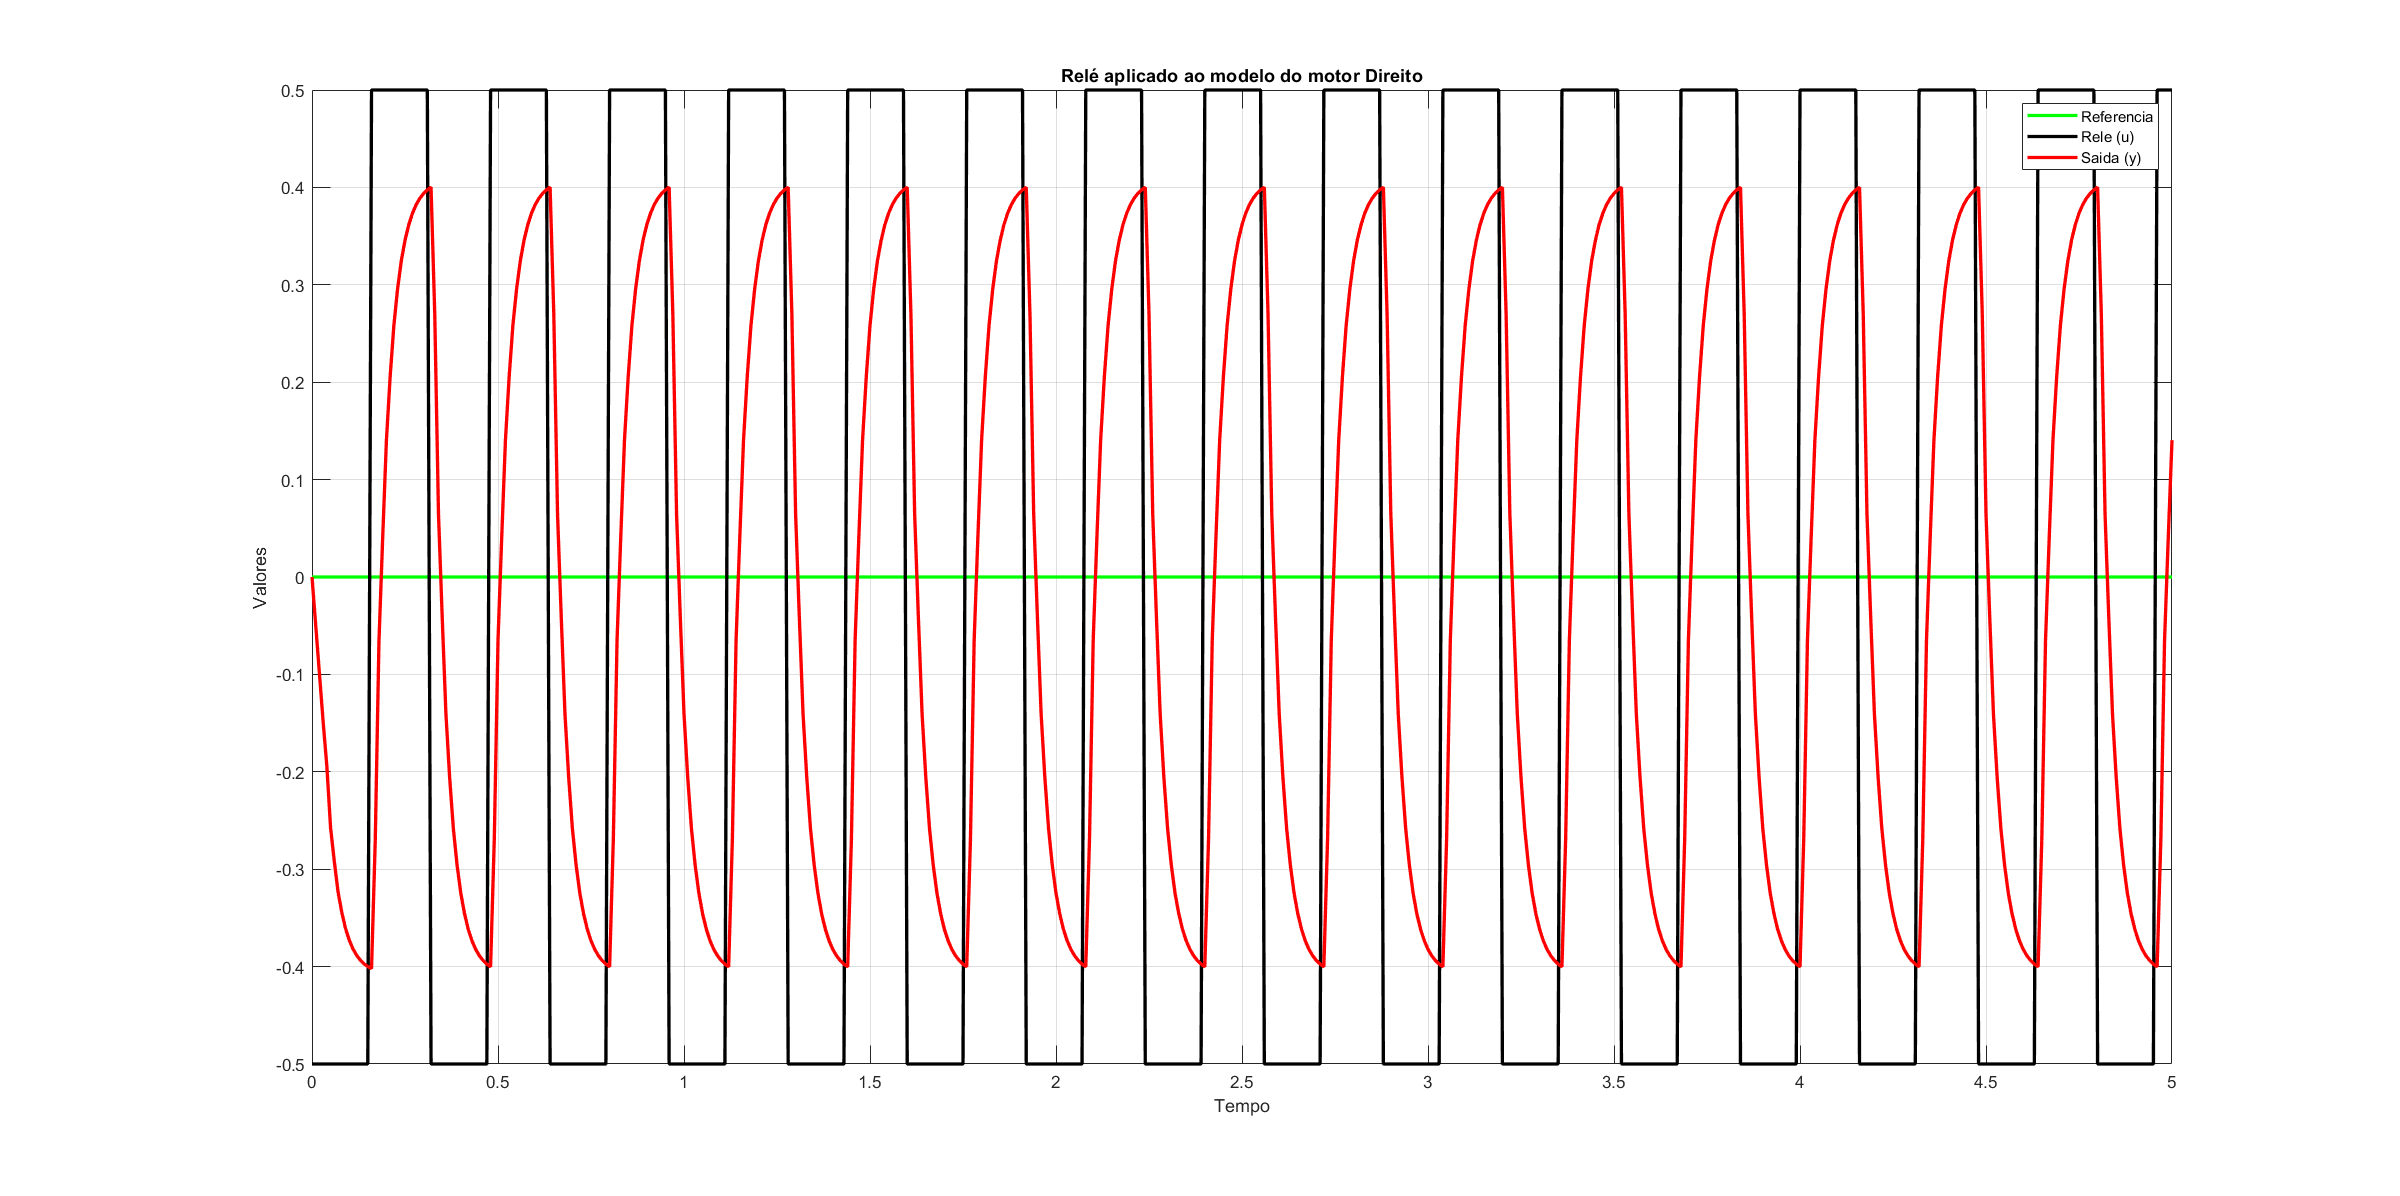
\includegraphics[width=16cm]{figuras/resultados/fig-motores/rele_motor_direito.png}
                    }{
                        \Fonte{O autor}
                    }	
            \end{figure}

            \begin{figure}[ht]
                \centering
                \Caption{\label{fig:rele-modelo-esquerdo} Relé no modelo do motor esquerdo}	
                    \UFCfig{}{
                        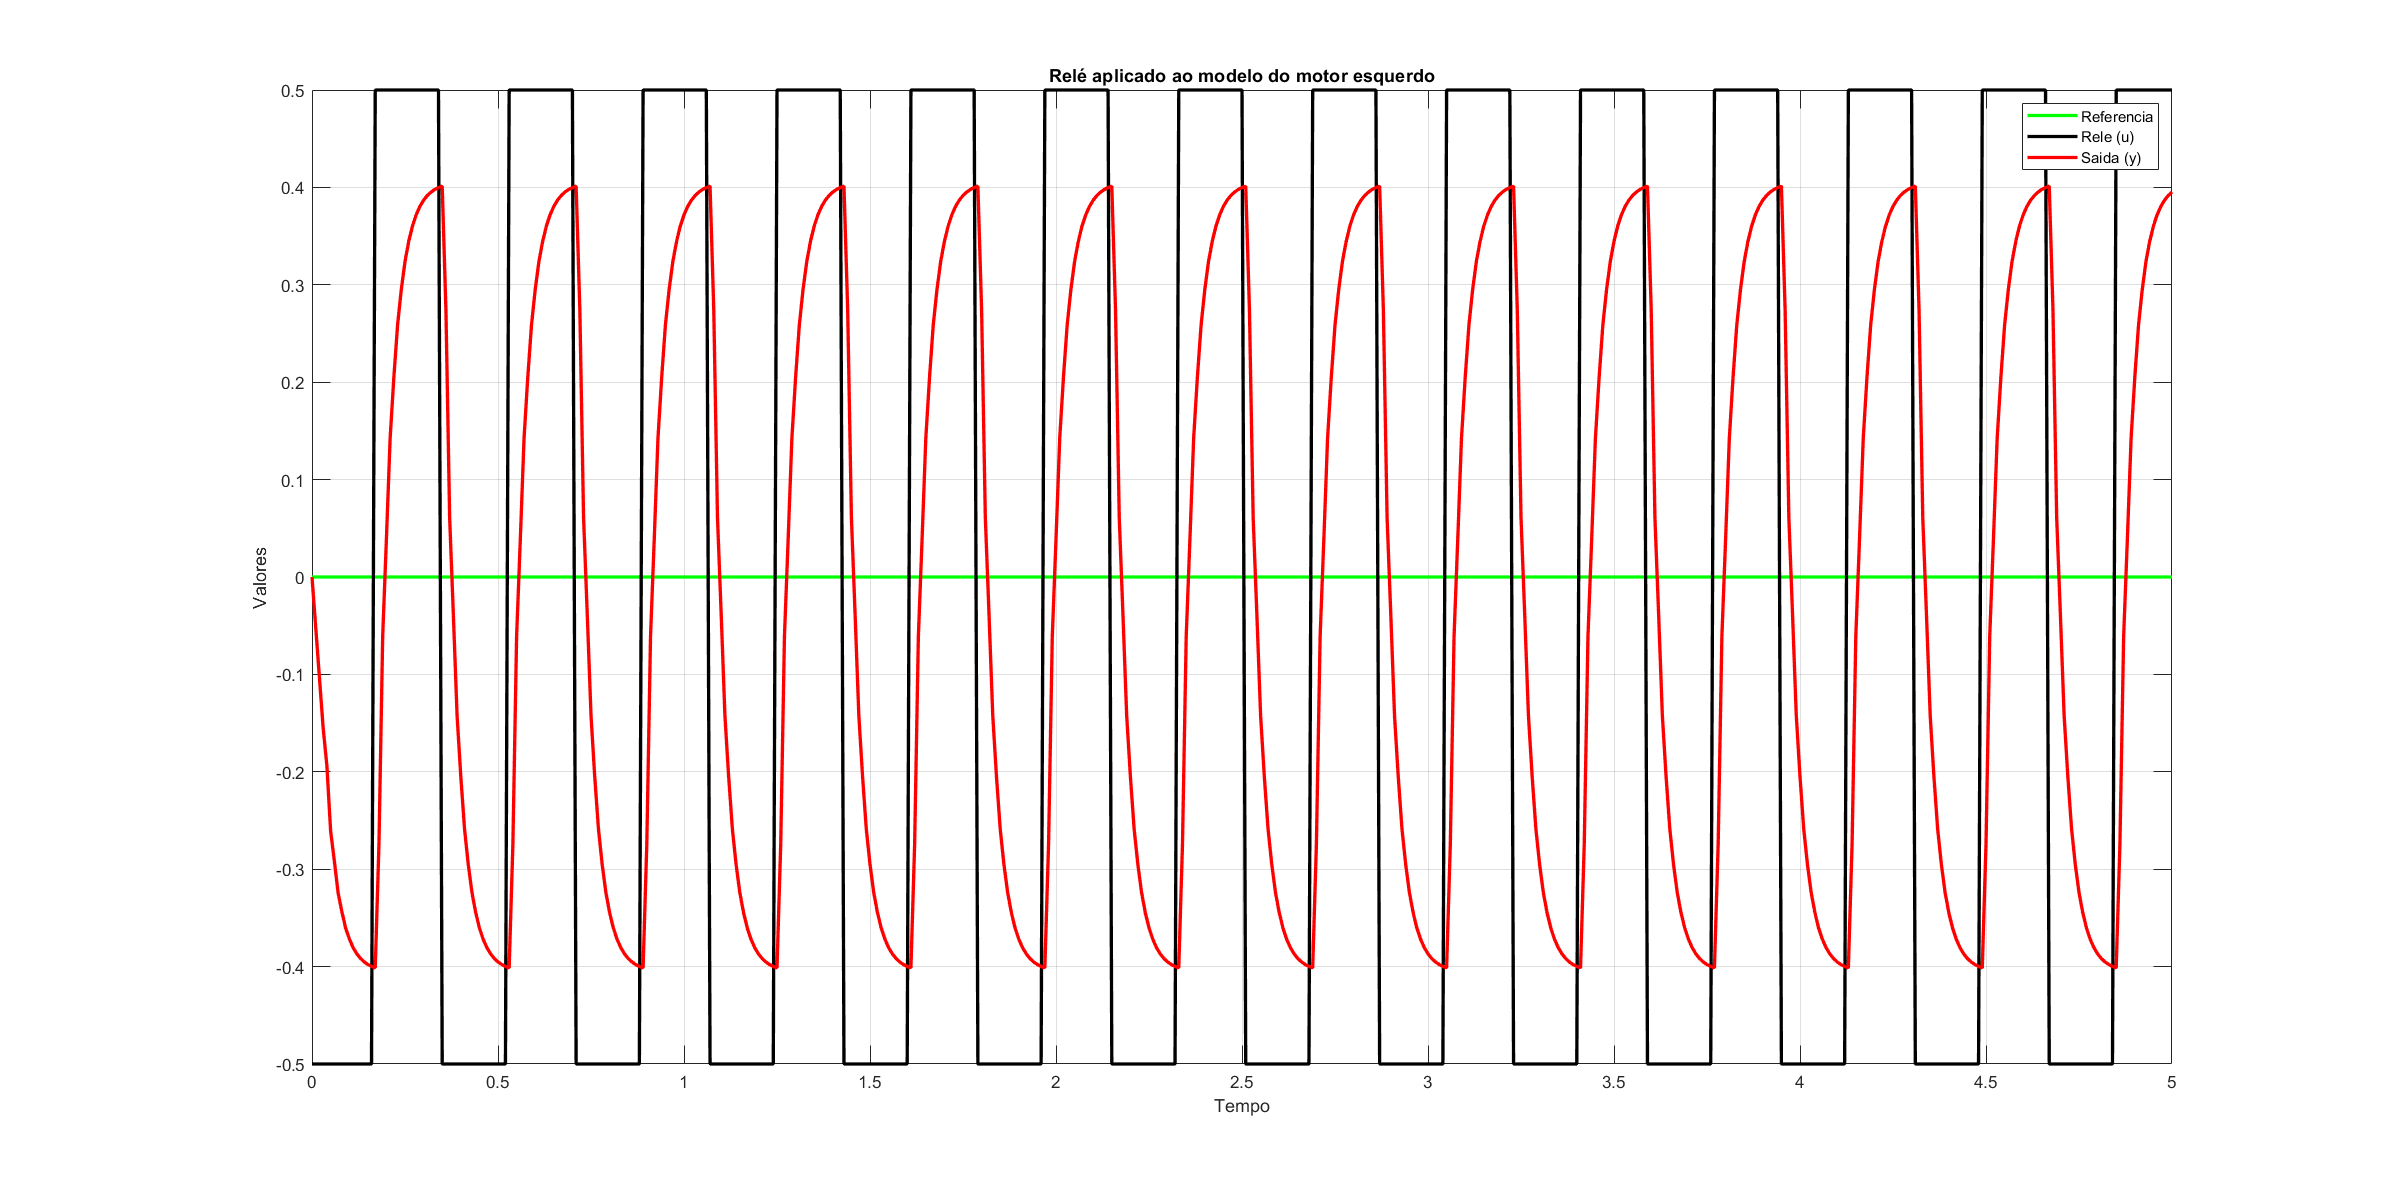
\includegraphics[width=16cm]{figuras/resultados/fig-motores/rele_motor_esquerdo.png}
                    }{
                        \Fonte{O autor}
                    }	
            \end{figure}

            \begin{table}[!htbp]	
				\centering
				\Caption{\label{tab:parametros-rele-motores} Parâmetros do Relé para os motores}
				\UFCtab{}{
					\begin{tabular}{ccc}
						\toprule
						Parâmetro/Motor & \( Direito \) & \( Esquerdo \) \\
						\midrule
						\( K_{u} \) & \( 1.5910 \) & \( 1.5864 \) \\
						\( T_{u} \)    & \( 0.3200 \) & \( 0.3600 \) \\
						\( a \)   & \( 0.4001 \) & \( 0.4013 \) \\
                        \( d \)   & \( 0.5000 \) & \( 0.5000 \) \\
                        \( \epsilon \)   & \( 0.4000 \) & \( 0.4000 \) \\
                        \( \omega_{u} \)   & \( 19.6350 \) & \( 17.4553 \) \\
						\bottomrule
					\end{tabular}
				}{
					\Fonte{O autor}
				}
			\end{table}

            Observa-se que os modelos possuem dinâmicas parecidas, porém não podem ser consideradas iguais de forma que os resultados da aplicação do relé resultam em parâmetros ligeiramente diferentes, o que resultará também en controladores com diferentes ganhos.

            Por fim, são projetados os controladores, cujos parâmetros $g_0$, $g_1$ e $g_2$ são obtidos para cada um dos motores e aplicados no robô e mostrados conforme a Tabela \ref{tab:parametros-controladores-motores}.

            \begin{table}[!htbp]	
				\centering
				\Caption{\label{tab:parametros-controladores-motores} Parâmetros do controlador para os motores}
				\UFCtab{}{
					\begin{tabular}{ccc}
						\toprule
						Parâmetro/Motor & \( Direito \) & \( Esquerdo \) \\
						\midrule
						\( g_0 \) & \( 2.2859 \) & \( 3.4699 \) \\
						\( g_1 \)    & \( -3.4750 \) & \( -5.4859 \) \\
						\( g_2 \)   & \( 1.3341 \) & \( 2.1822 \) \\
						\bottomrule
					\end{tabular}
				}{
					\Fonte{O autor}
				}
			\end{table}

            Os testes de controle foram conduzidos aplicando inicialmente um patamar de referência e depois aplicando três patamares, conforme apresentado nas Figuras \ref{fig:controle-motor-direito-1-patamar} a \ref{fig:controle-motor-esquerdo-3-patamares}. Suas métricas são então apresentadas nas Tabelas \ref{tab:metricas-controle-1-patamar} e \ref{tab:metricas-controle-3-patamares}.

            As Figuras \ref{fig:controle-motor-direito-1-patamar} a \ref{fig:controle-motor-esquerdo-3-patamares} também contém dois \textit{plots}. No primeiro está contido o sinal de referência, em azul, a resposta dos motores, em preto, e o erro do sistema, em rosa. No segundo \textit{plot} está contida a o sinal de controle produzido por cada um dos controladores \gls{PID} e que corresponde à entrada do motor.

            \begin{figure}[ht]
                \centering
                \Caption{\label{fig:controle-motor-direito-1-patamar} PID no motor direito para 1 patamar}	
                    \UFCfig{}{
                        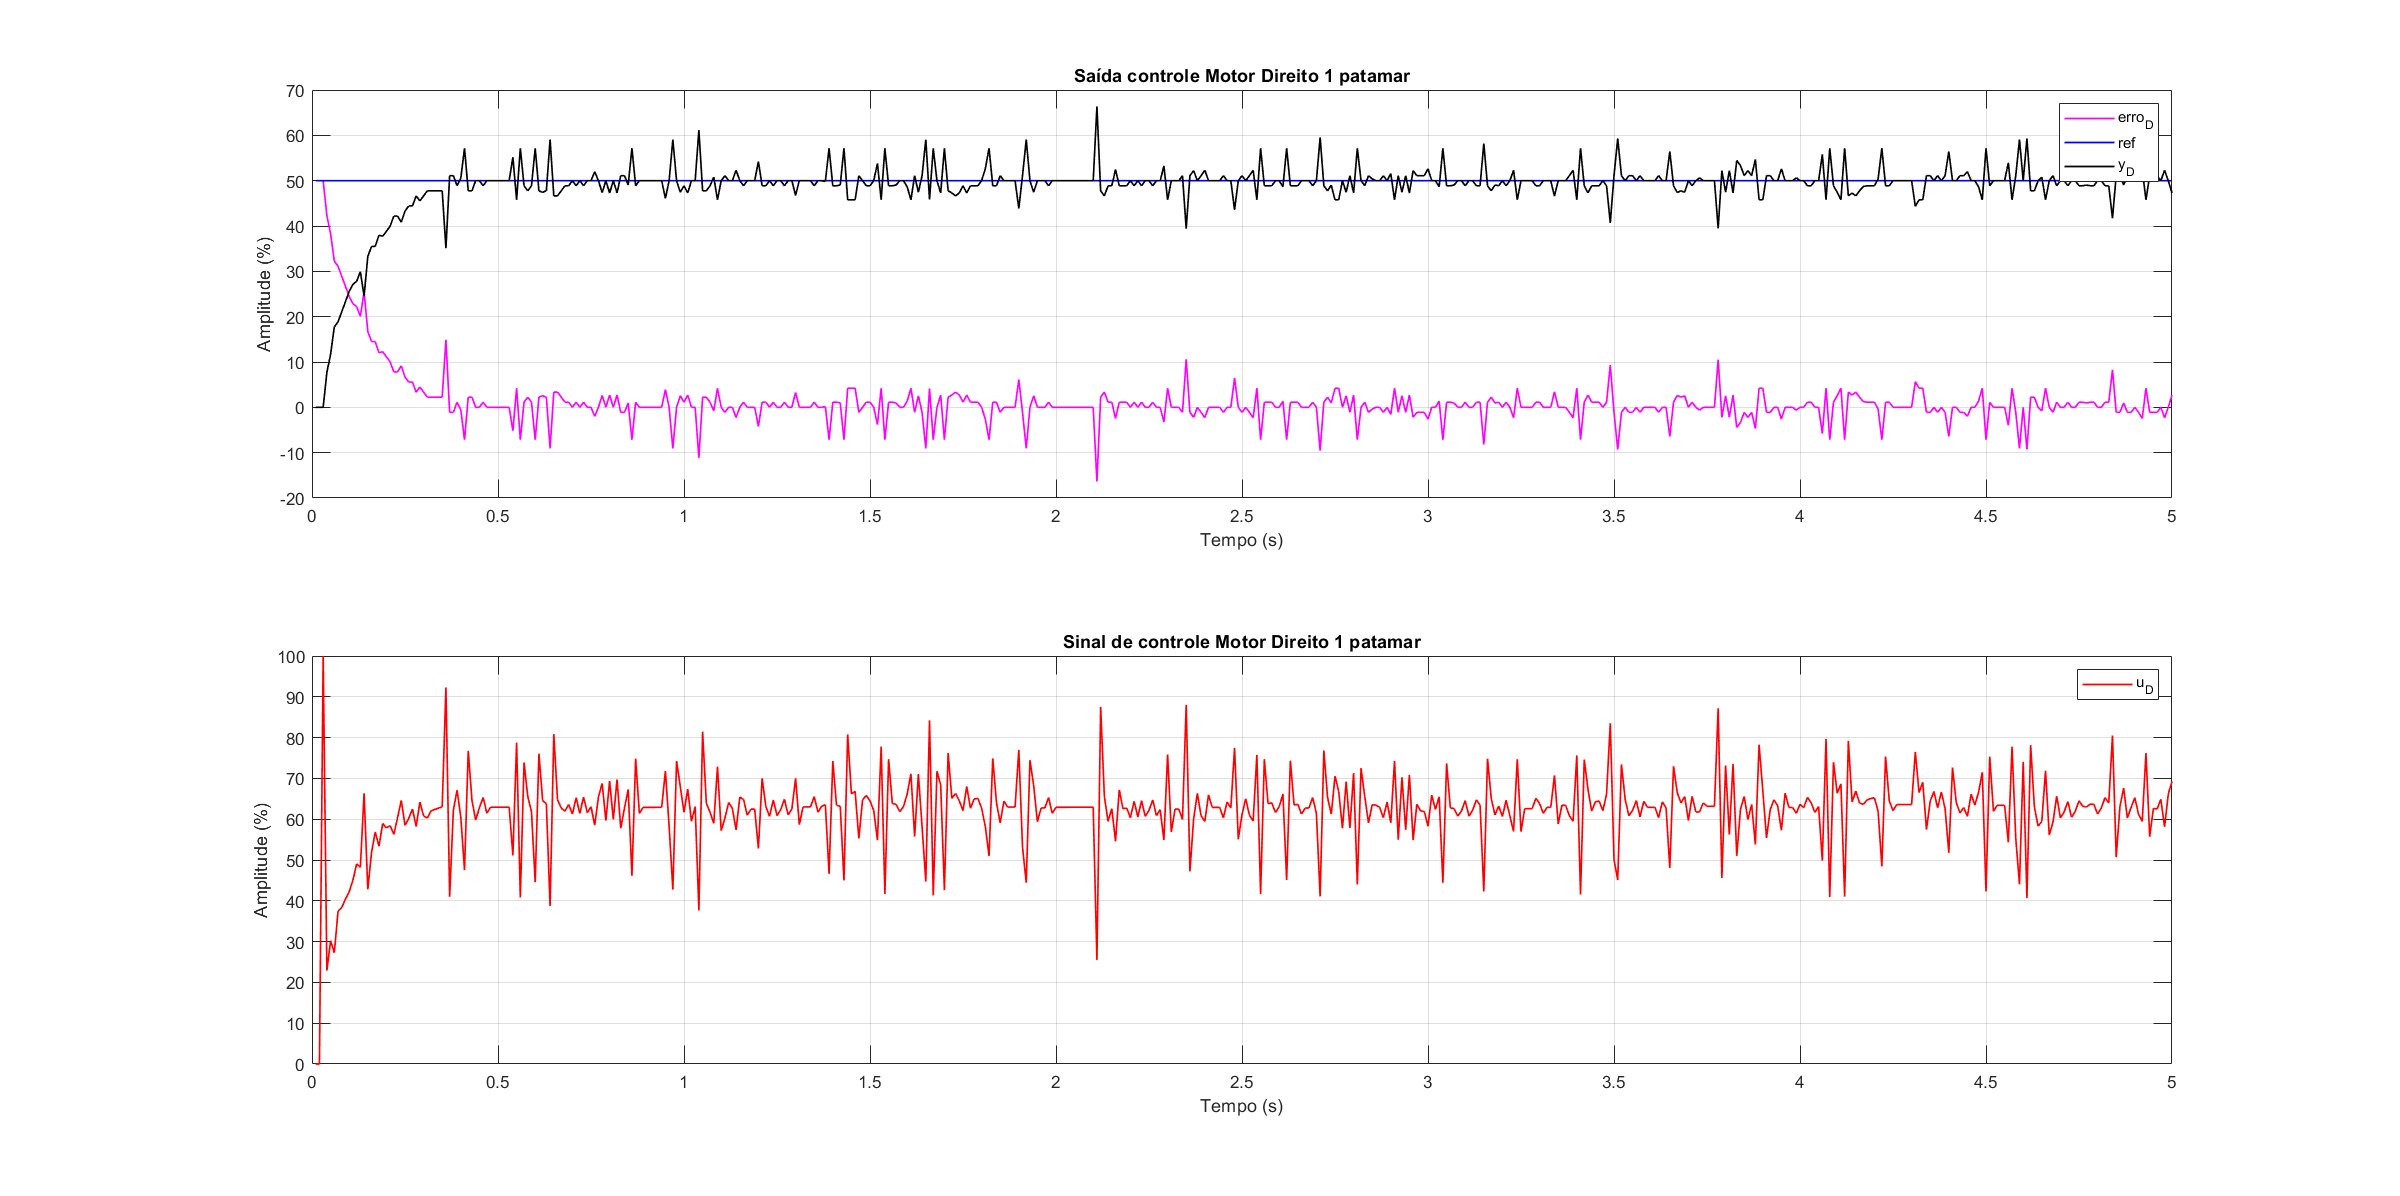
\includegraphics[width=16cm]{figuras/resultados/fig-motores/PID_direito_1_patamar_sem_ressintonia.png}
                    }{
                        \Fonte{O autor}
                    }	
            \end{figure}

            \begin{figure}[ht]
                \centering
                \Caption{\label{fig:controle-motor-esquerdo-1-patamar} PID no motor esquerdo para 1 patamar}	
                    \UFCfig{}{
                        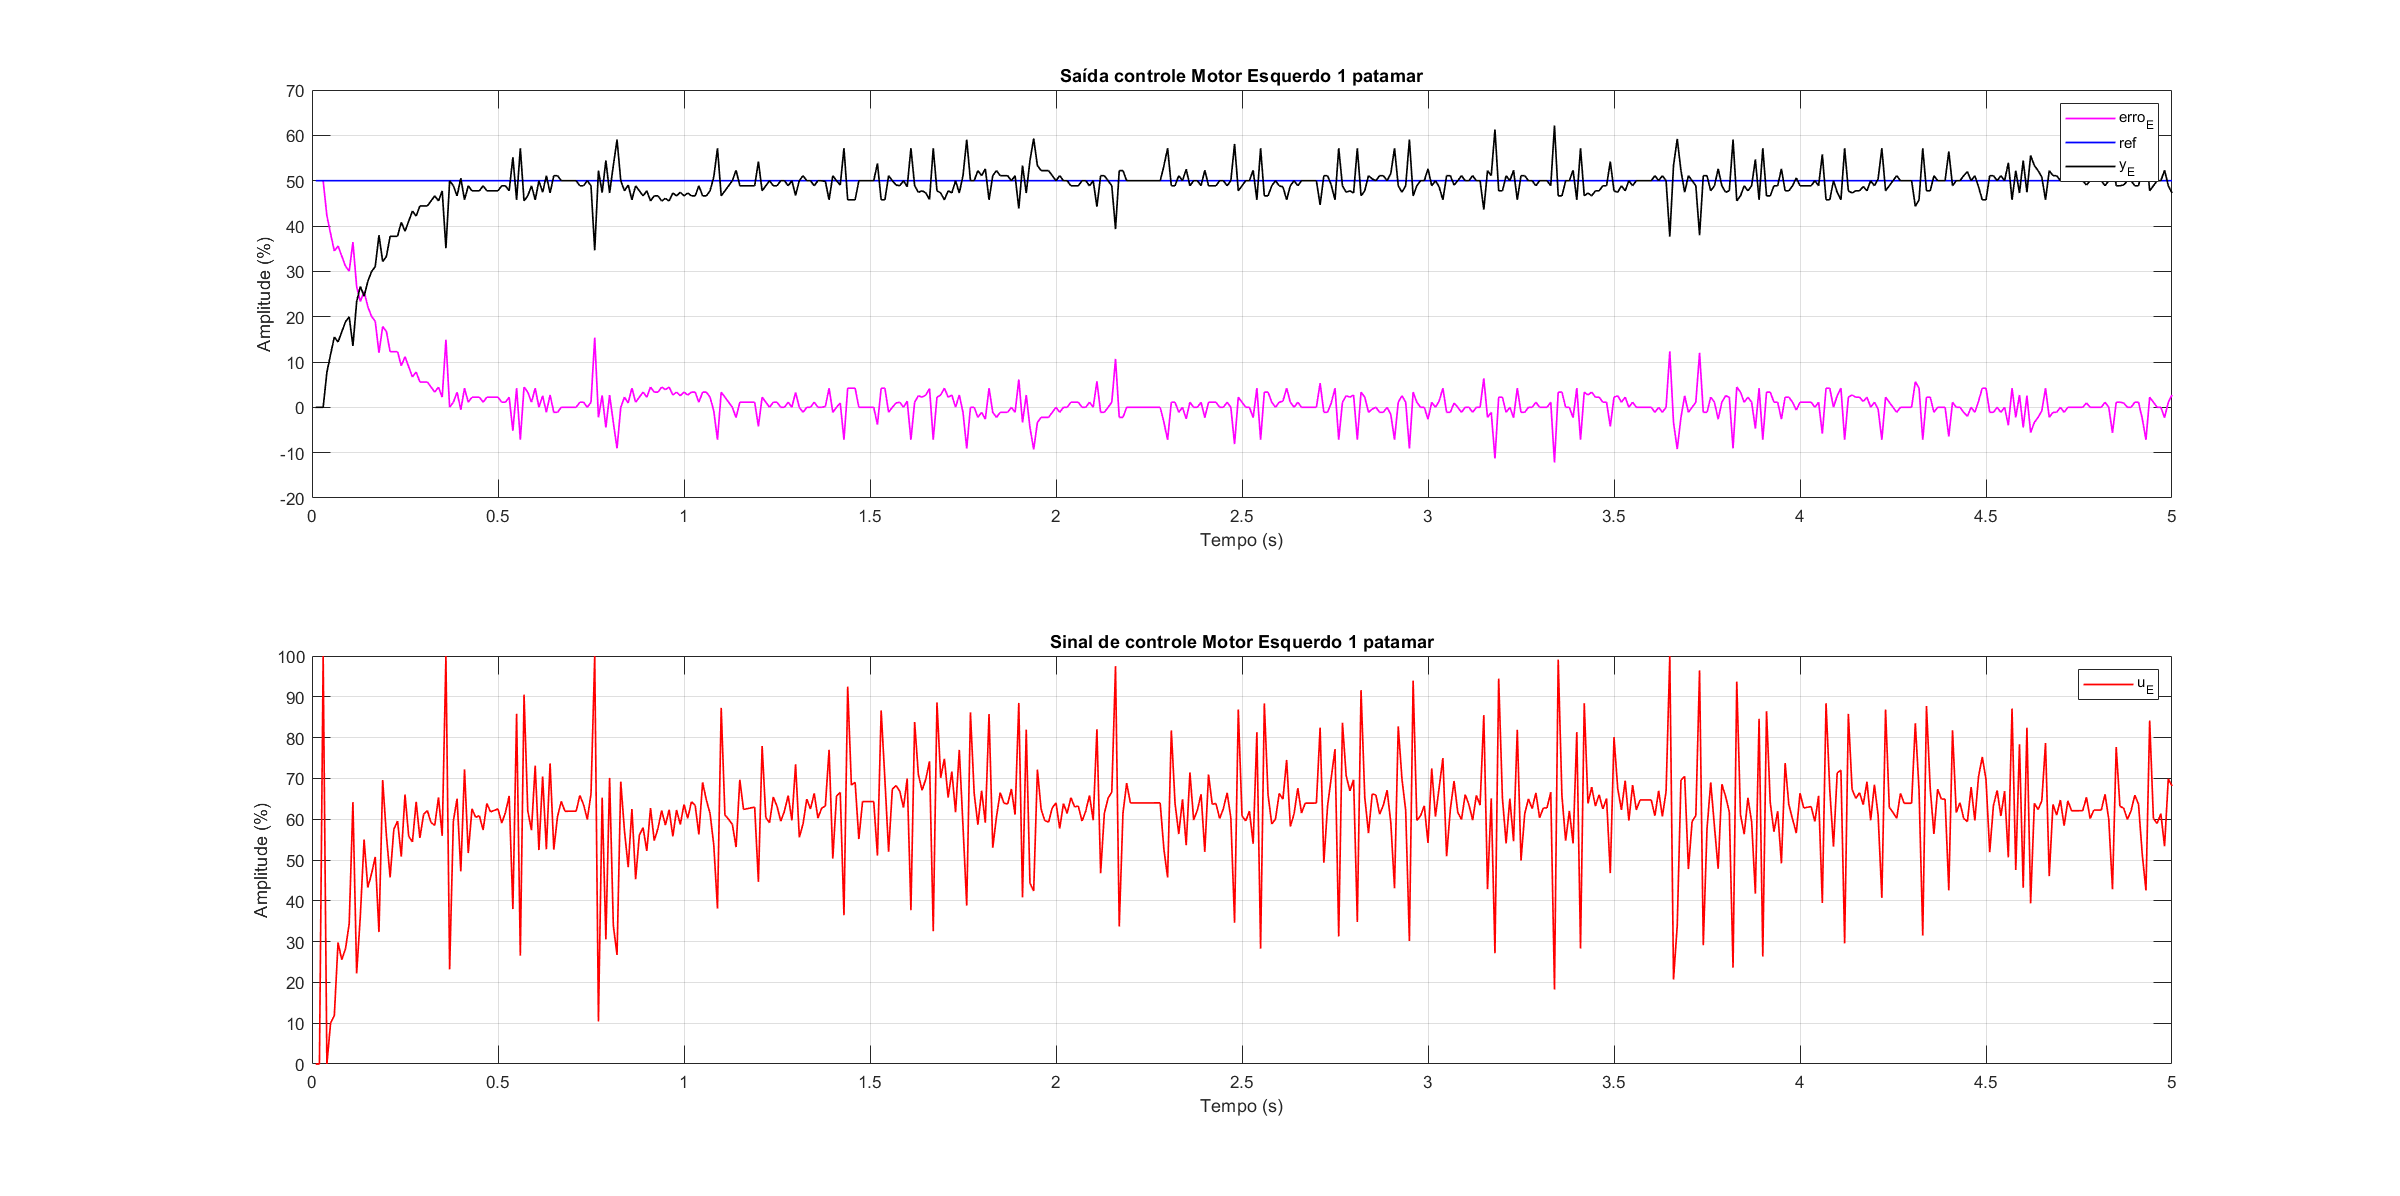
\includegraphics[width=16cm]{figuras/resultados/fig-motores/PID_esquerdo_1_patamar_sem_ressintonia.png}
                    }{
                        \Fonte{O autor}
                    }	
            \end{figure}

            \begin{figure}[ht]
                \centering
                \Caption{\label{fig:controle-motor-direito-3-patamares} PID no motor direito para 3 patamares}	
                    \UFCfig{}{
                        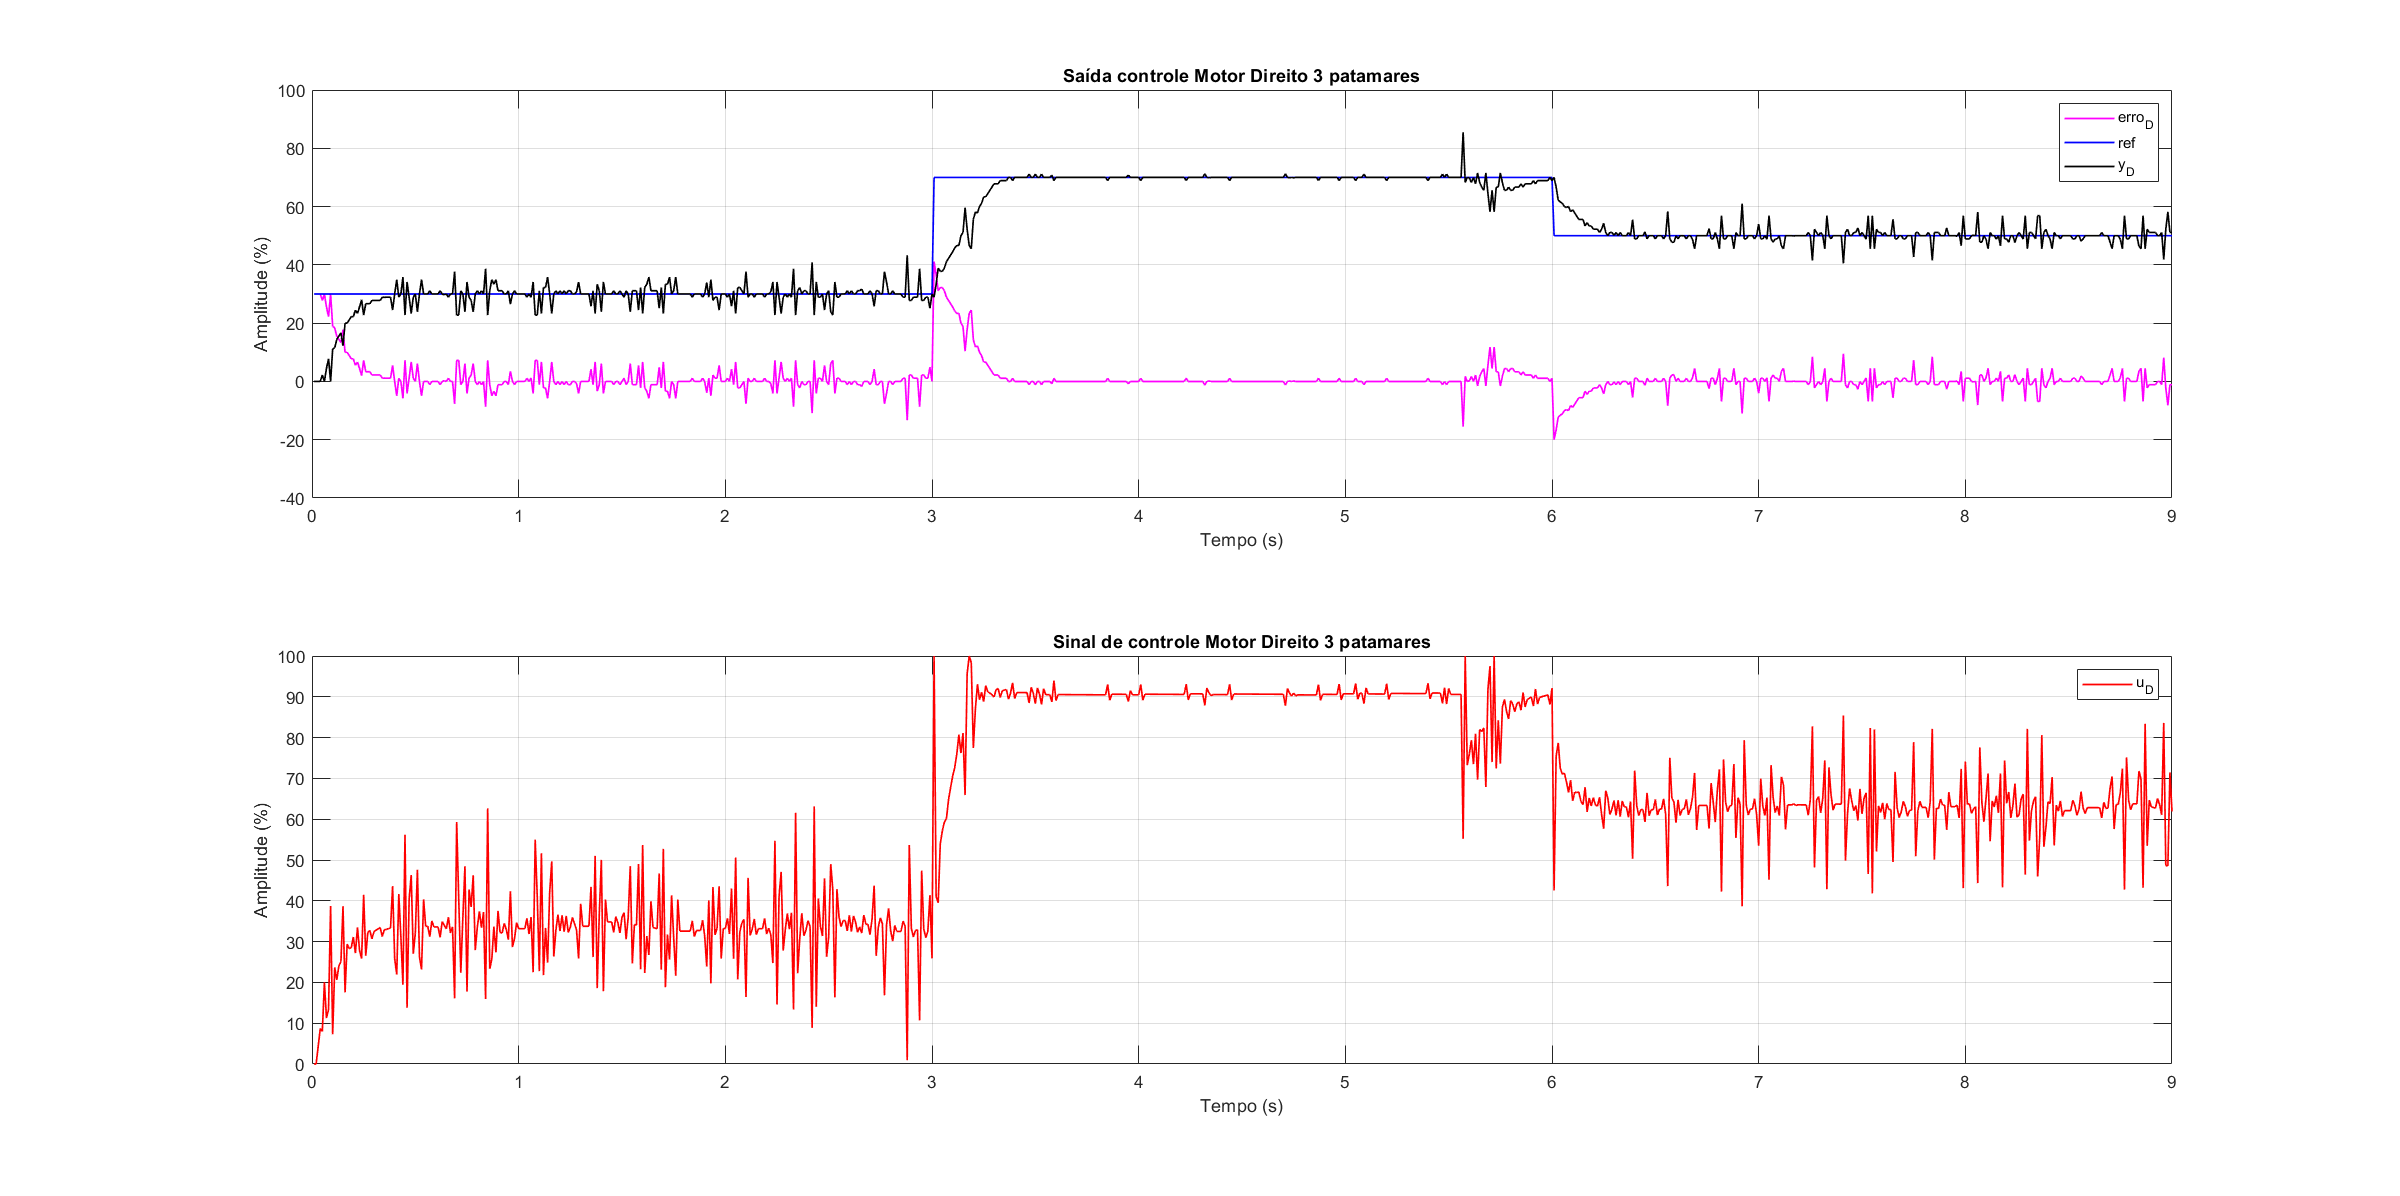
\includegraphics[width=16cm]{figuras/resultados/fig-motores/PID_direito_3_patamar_sem_ressintonia.png}
                    }{
                        \Fonte{O autor}
                    }	
            \end{figure}

            \begin{figure}[ht]
                \centering
                \Caption{\label{fig:controle-motor-esquerdo-3-patamares} PID no motor esquerdo para 3 patamares}	
                    \UFCfig{}{
                        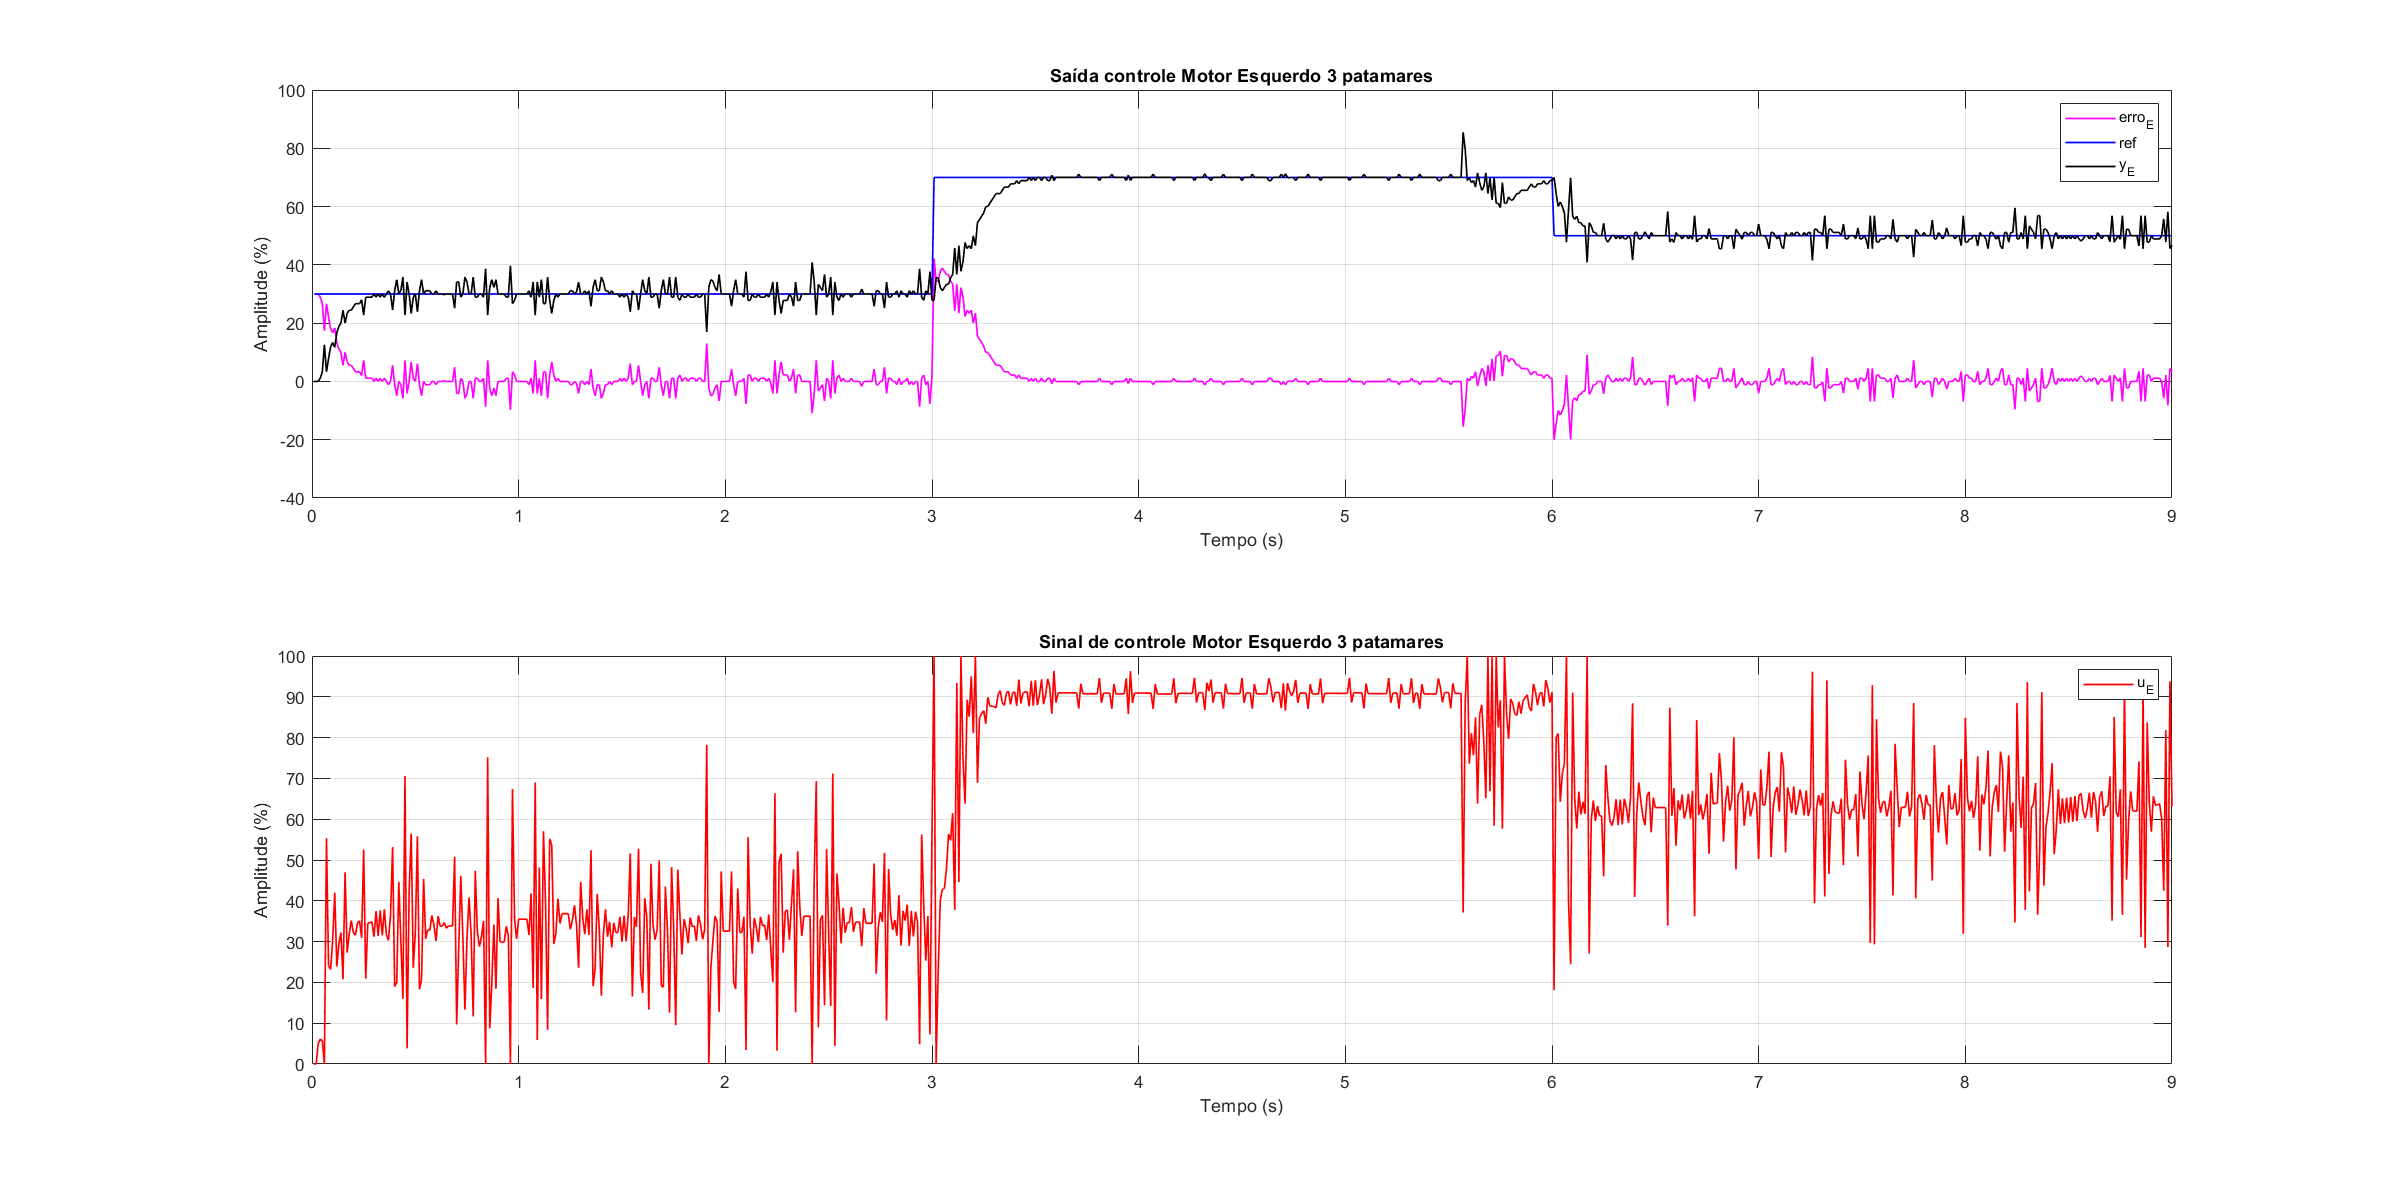
\includegraphics[width=16cm]{figuras/resultados/fig-motores/PID_esquerdo_3_patamar_sem_ressintonia.png}
                    }{
                        \Fonte{O autor}
                    }	
            \end{figure}

            \begin{table}[!htbp]	
				\centering
				\Caption{\label{tab:metricas-controle-1-patamar} Resultados de controle para 1 patamar}
				\UFCtab{}{
					\begin{tabular}{ccc}
						\toprule
						    Métrica/Motor & Direito & Esquerdo \\
						\midrule
                            Sobressinal (\%) & \( 2.2064 \) & \( 24.3352 \) \\
                            IAE & \( 1436.6 \) & \( 1700.1 \) \\
                            Variância da saída & \( 43.9402 \) & \( 50.9943 \) \\
                            Variância da do controle & \( 94.5763 \) & \( 214.4647 \) \\
                            Tempo de assentamento (s) & \( 0.3600 \) & \( 0.3900 \) \\
						\bottomrule
					\end{tabular}
				}{
					\Fonte{O autor}
				}
			\end{table}

            \begin{table}[!htbp]	
				\centering
				\Caption{\label{tab:metricas-controle-3-patamares} Resultados de controle para 3 patamares}
				\UFCtab{}{
					\begin{tabular}{ccc}
						\toprule
						    Métrica/Motor & Direito & Esquerdo \\
						\midrule
                            Sobressinal do primeiro patamar (\%) & \( 3.7327 \) & \( 0.0280 \) \\
                            IAE & \( 2300.6 \) & \( 2502.7 \) \\
                            Variância da saída & \( 290.6884 \) & \( 278.6816 \) \\
                            Variância da do controle & \( 590.3571 \) & \( 656.2484 \) \\
                            Tempo de assentamento (s) do primeiro patamar & \( 0.3700 \) & \( 0.3300 \) \\
						\bottomrule
					\end{tabular}
				}{
					\Fonte{O autor}
				}
			\end{table}

            % Com os dados apresentados pode-se observar que apesar de uma variância relativamente alta nos sinais de controle observa-se que a saída dos sistemas mantém-se controlada mesmo em mudanças de patamares de forma que a variância no sinal de saída é consideralvelmente menor que a variância do controle, seja para 1 ou 3 patamares. Observa-se também, que os motores apresentam tempos de assentamentos parecidos e próximos o que é de vital importância para a manutenção do robô dentro dos percursos e comportamentos desejados.

            A partir dos dados apresentados nas Figuras \ref{fig:controle-motor-direito-1-patamar} a \ref{fig:controle-motor-esquerdo-3-patamares}, observa-se que embora os sinais de controle apresentem variância relativamente elevada, as saídas dos sistemas permanecem adequadamente controladas, inclusive durante as mudanças entre diferentes patamares de referência. Em ambos os testes, realizados com um e três patamares, a variância do sinal de saída é consideravelmente inferior à variância do respectivo sinal de controle, indicando que as oscilações associadas à ação de controle não se refletem com a mesma intensidade na resposta dos motores. Verifica-se, ainda, que os motores apresentam tempos de assentamento semelhantes e próximos entre si. Tal característica é fundamental para a coordenação de movimentos do robô, uma vez que caso haja diferenças significativas entre as respostas das rodas podem ser provocados desvios de trajetória e comprometer a execução dos movimentos desejados. Portanto, a proximidade entre os tempos de assentamento contribui para a manutenção do \textit{micromouse} nos percursos planejados.

    \section{Testes realizados para as variáveis globais} \label{sec:res-global}

        % Assim, tendo sido implementados os controladores de cada motor procedeu-se com os testes e ensaios para os controladores supervisórios. Como tais controladores atuam em conjunto com as malhas internas é necessário que as coletas de dados sejam realizadas levando em consideração a dinâmica introduzida e modificada por tais malhas, isto é, as co letas de dados realizadas a partir de então são feitas já com os motores sendo devidamente controlados.

        Após a implementação dos controladores individuais de cada motor, procedeu-se à realização dos testes destinados ao projeto dos controladores supervisórios. Como essas malhas de nível superior atuam em conjunto com as malhas internas de controle dos motores, a coleta de dados deve considerar a dinâmica resultante dessa estrutura. Dessa forma, os dados utilizados nas etapas seguintes são obtidos com os motores operando sob ação dos respectivos controladores individuais. Assim, essa abordagem permite que a identificação e o projeto das malhas supervisórias sejam realizados com base no comportamento efetivo do sistema, já considerando as alterações dinâmicas introduzidas.


        \subsection{Identificação das variáveis globais} \label{sec:res-id-global}

            Para a identificação das malhas globais são também aplicados sinais \gls{PRBS} em cada uma das malhas, semelhantemente ao realizado para os motores. A diferença residirá no valor da referência $R$ aplicada ao sinal de velocidade angular, que nesse caso será o valor adimensional de $\frac{\pi}{2}$. Para a malha de velocidade linear é seguido com $R = 50\%$. As Figuras \ref{fig:resposta-prbs-v-linear} e \ref{fig:resposta-prbs-w-angular} apresentam os valores obtidos na coleta de dados para o sinal de velocidade linear e angular respectivamente. Nestas figuras, bem como nas demais que aparecem nas seções seguintes, foi utilizado o mesmo esquema de cores descrito na Seção \ref{sec:res-controle-motores}.

            \begin{figure}[ht]
                \centering
                \Caption{\label{fig:resposta-prbs-v-linear} Resposta a entrada PRBS de $V$}	
                    \UFCfig{}{
                        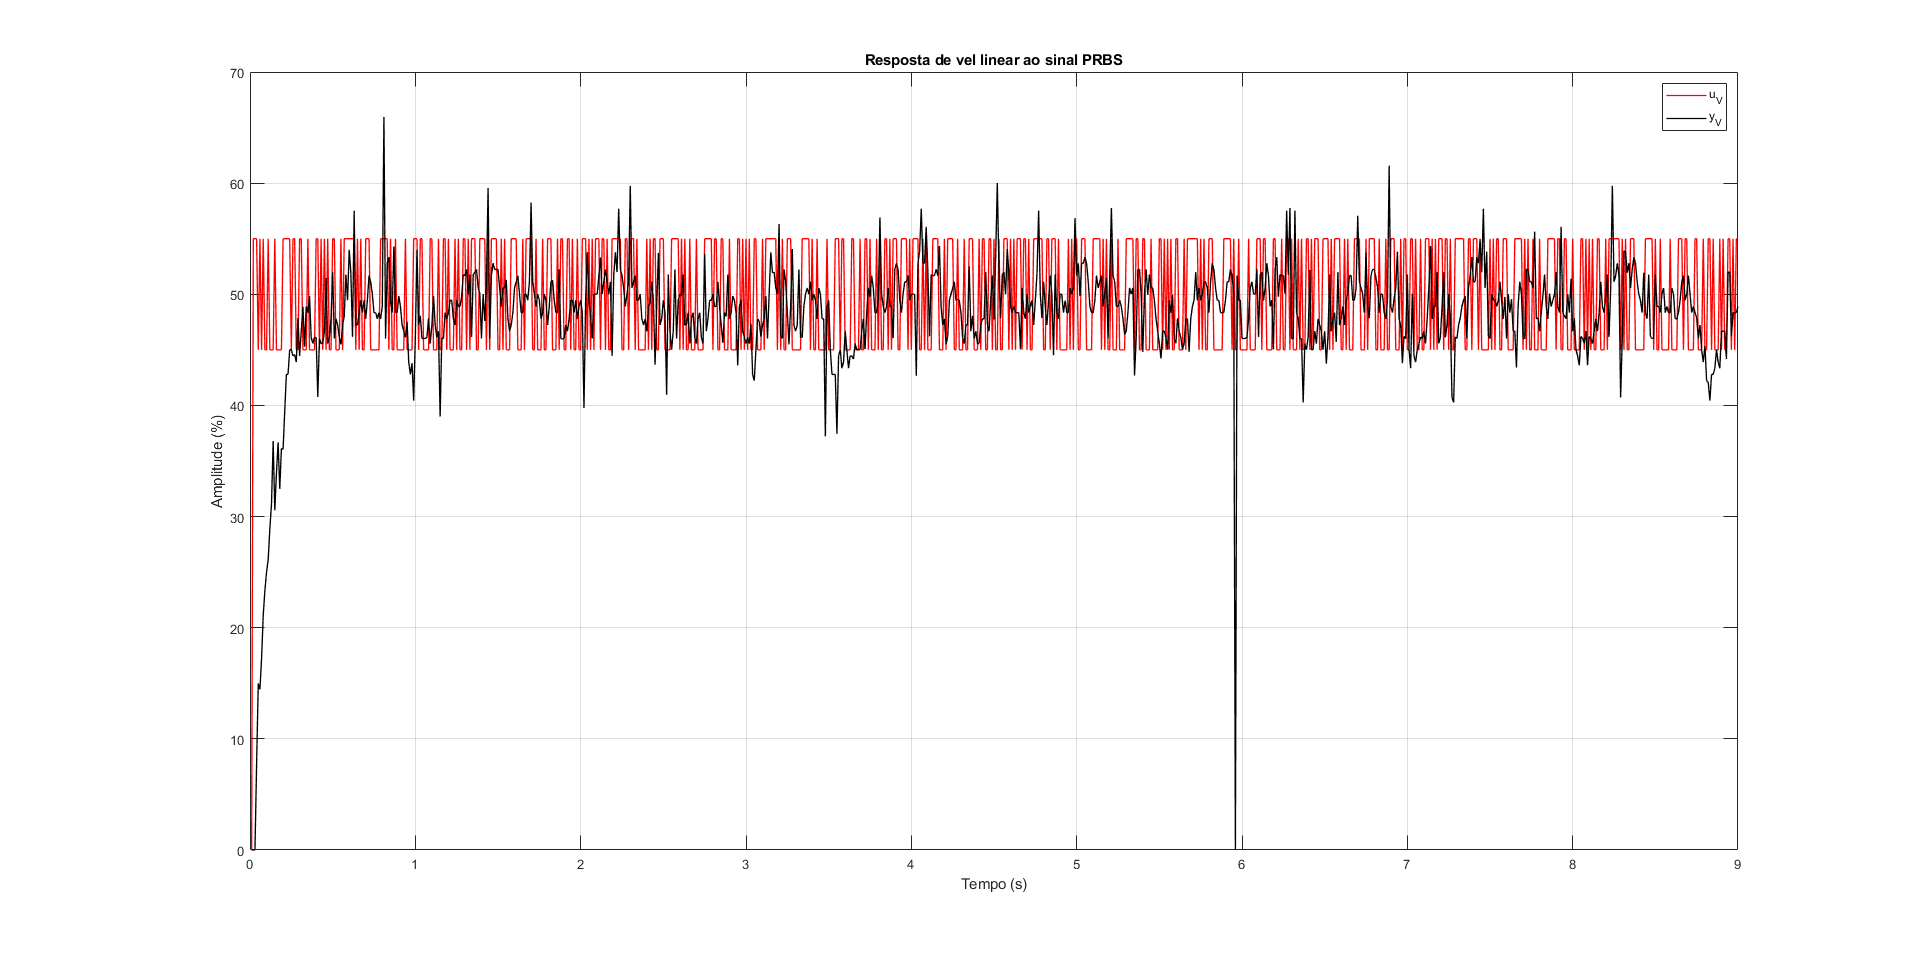
\includegraphics[width=16cm]{figuras/resultados/fig-global/resp-prbs-vel-lin.png}
                    }{
                        \Fonte{O autor}
                    }	
            \end{figure}

            \begin{figure}[ht]
                \centering
                \Caption{\label{fig:resposta-prbs-w-angular} Resposta a entrada PRBS de $\omega$}	
                    \UFCfig{}{
                        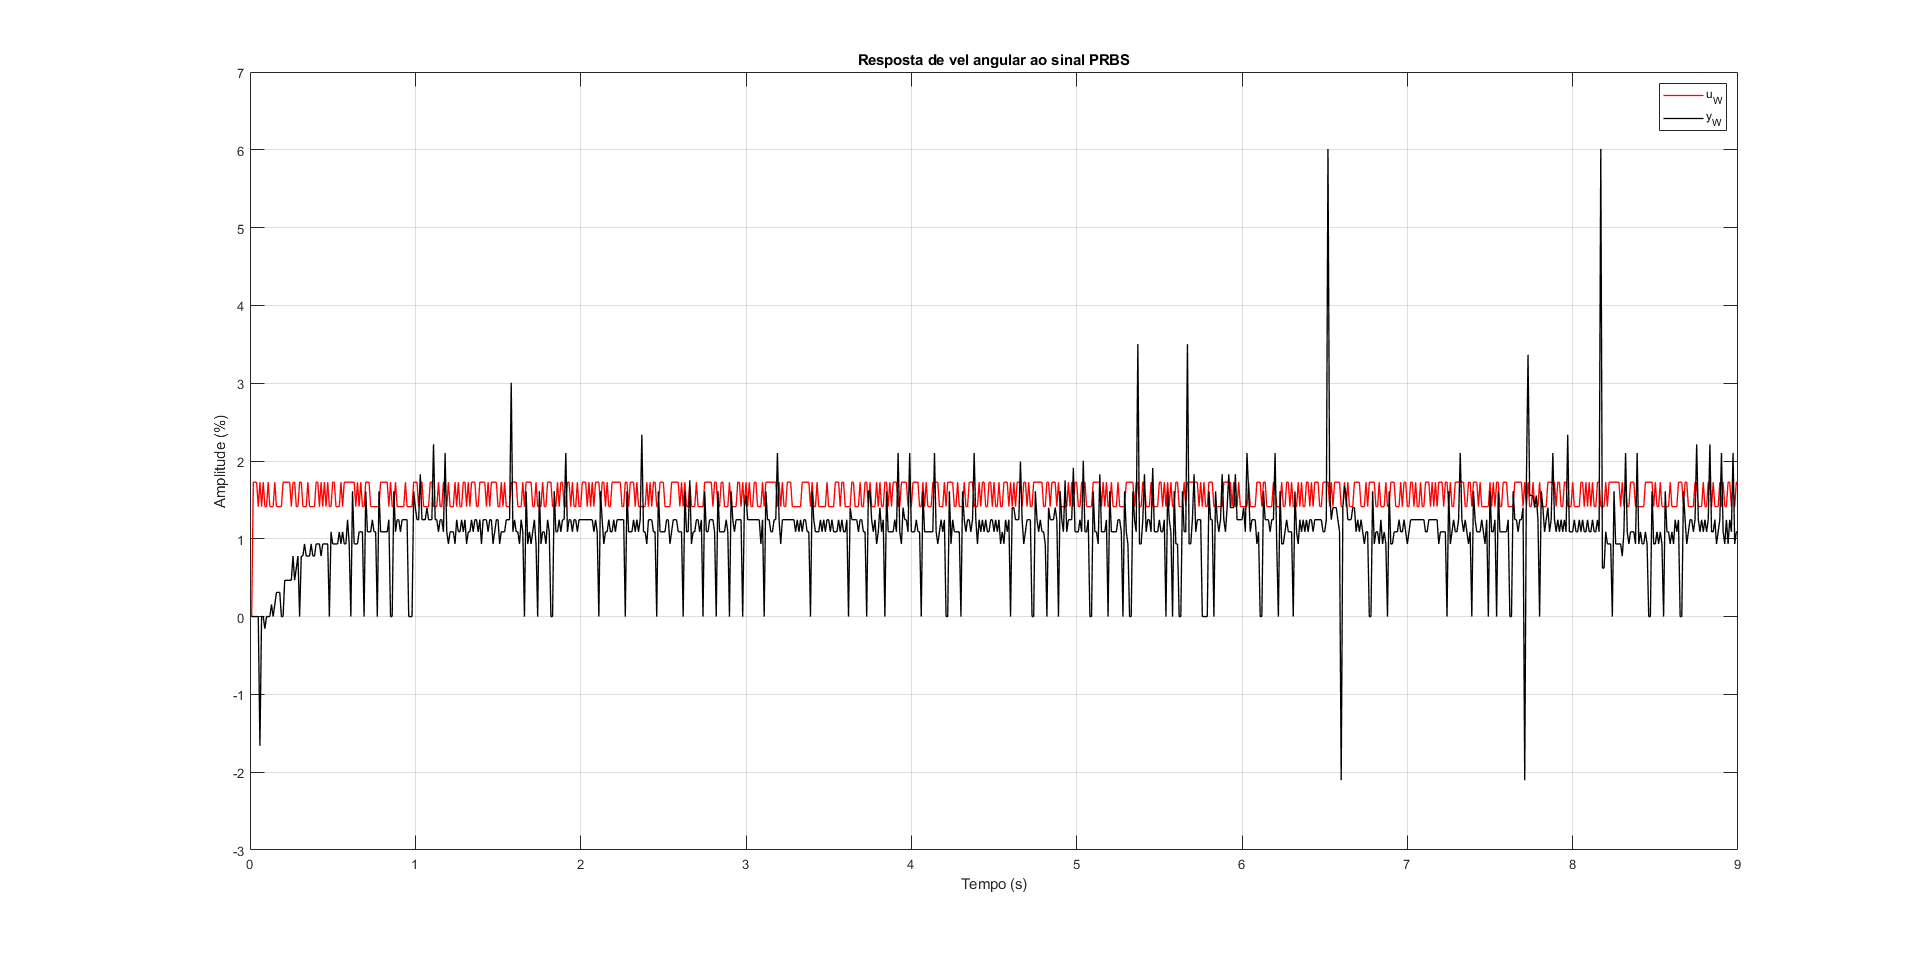
\includegraphics[width=16cm]{figuras/resultados/fig-global/resp-prbs-w-ang.png}
                    }{
                        \Fonte{O autor}
                    }	
            \end{figure}

            Semelhantemente ao realizado nos motores, é aplicado o método \gls{MQNR} para identificação das malhas. Os resultados em testes de validação obtidos são apresentados nas Figuras \ref{fig:identificacao-global-v-linear} e \ref{fig:identificacao-global-w-angular} bem como os coeficientes encontrados, os quais estão presentes na Tabela \ref{tab:coeficientes-identificacao-global}.

            \begin{figure}[ht]
                \centering
                \Caption{\label{fig:identificacao-global-v-linear} Resultado da identificação da malha $V$ pelo MQNR}	
                    \UFCfig{}{
                        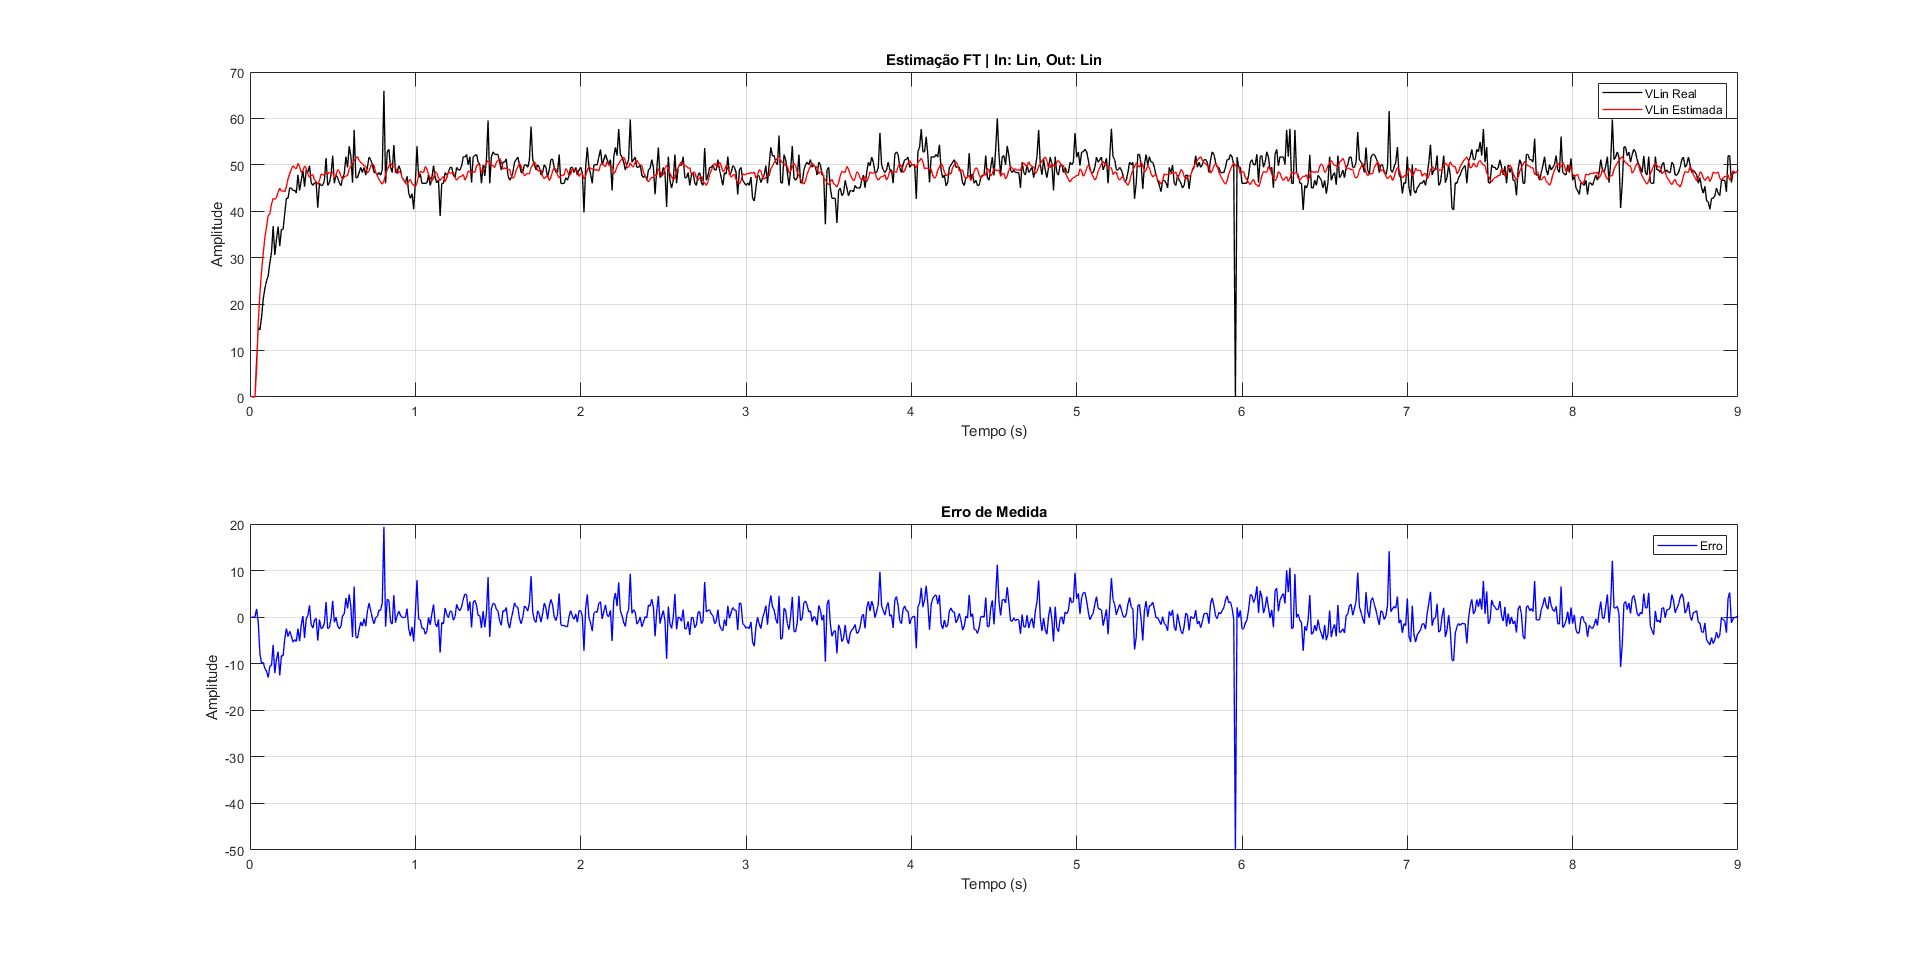
\includegraphics[width=16cm]{figuras/resultados/fig-global/identifica-vel-lin.png}
                    }{
                        \Fonte{O autor}
                    }	
            \end{figure}

            \begin{figure}[ht]
                \centering
                \Caption{\label{fig:identificacao-global-w-angular} Resultado da identificação da malha $\omega$ pelo MQNR}	
                    \UFCfig{}{
                        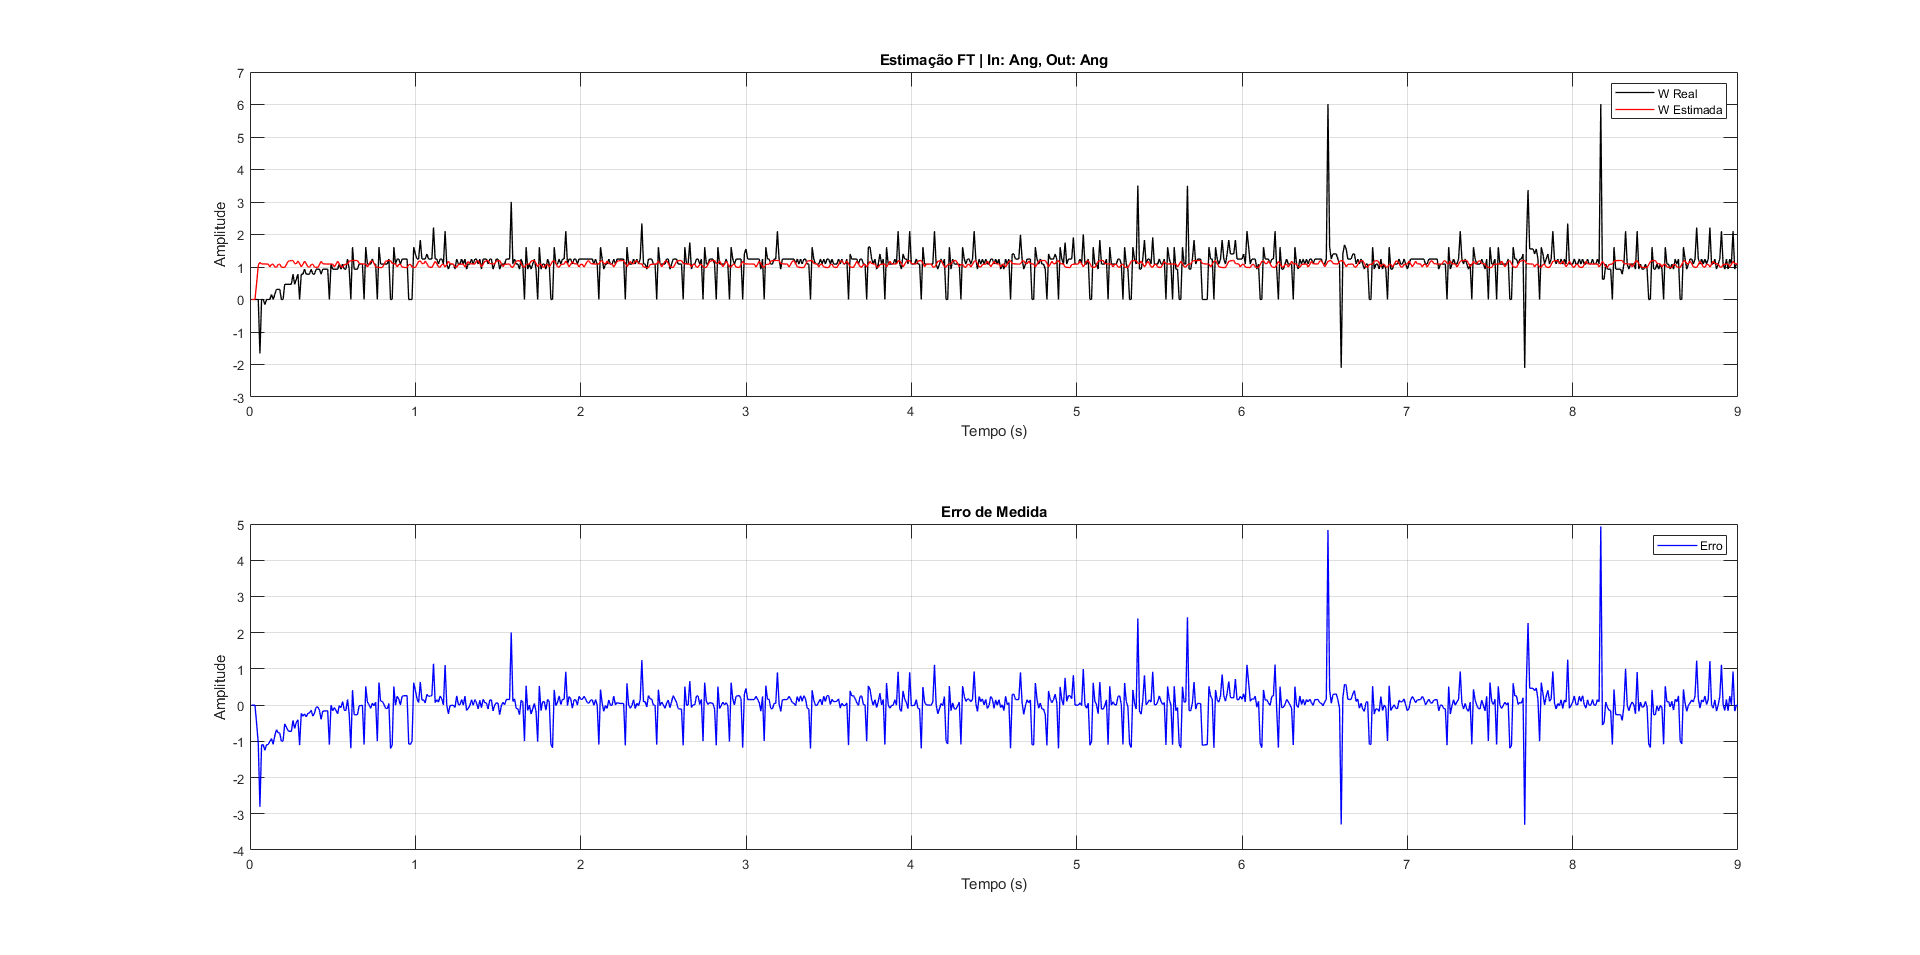
\includegraphics[width=16cm]{figuras/resultados/fig-global/identifica-w-ang.png}
                    }{
                        \Fonte{O autor}
                    }	
            \end{figure}

            \begin{table}[!htbp]	
				\centering
				\Caption{\label{tab:coeficientes-identificacao-global} Coeficientes dos modelos das malhas globais}
				\UFCtab{}{
					\begin{tabular}{ccc}
						\toprule
						Coeficiente/Malha & \( V \) & \( \omega  \) \\
						\midrule
						\( a_1 \) & \( -0.4089 \) & \( -0.1054 \) \\
						\( a_2 \)    & \( -0.3344 \) & \( -0.0578 \) \\
						\( b_1 \)   & \( 0.1094 \) & \( 0.2874 \) \\
                        \( b_2 \)   & \( 0.1397 \) & \( 0.2940 \) \\
						\bottomrule
					\end{tabular}
				}{
					\Fonte{O autor}
				}
			\end{table}

        \subsection{Controle aplicado nas variáveis globais} \label{sec:res-controle-global}

            Tendo sido modeladas as malhas de velocidade linear ($V$) e velocidade angular ($\omega$) é realizado a aplicação do método do Relé novamente, para cada uma das malhas, como apresentado nas Figuras \ref{fig:rele-vel-linear} e \ref{fig:rele-w-angular}, em seguida são determinados seus parâmetros os quais estão sintetizados na tabela \ref{tab:parametros-rele-global}.

            \begin{figure}[ht]
                \centering
                \Caption{\label{fig:rele-vel-linear} Aplicação do relé na malha $V$}	
                    \UFCfig{}{
                        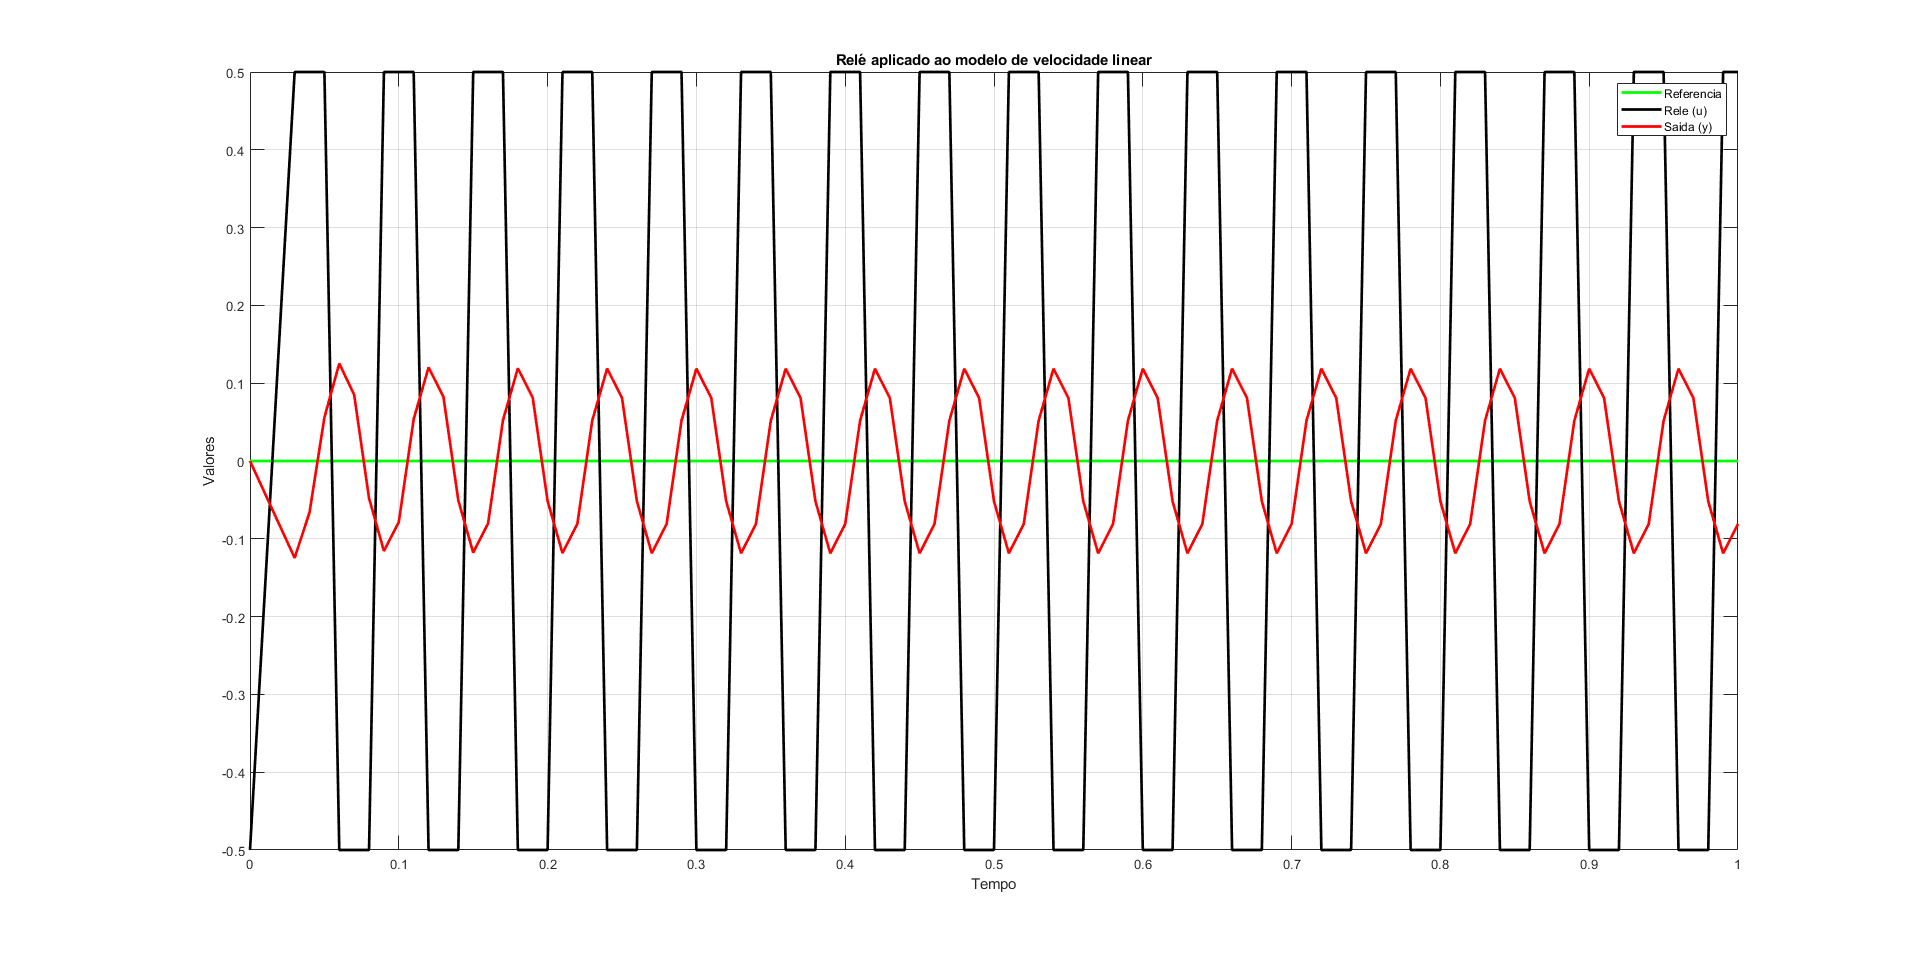
\includegraphics[width=16cm]{figuras/resultados/fig-global/rele-vel-lin.png}
                    }{
                        \Fonte{O autor}
                    }	
            \end{figure}

            \begin{figure}[ht]
                \centering
                \Caption{\label{fig:rele-w-angular} Aplicação do relé na malha $\omega$}	
                    \UFCfig{}{
                        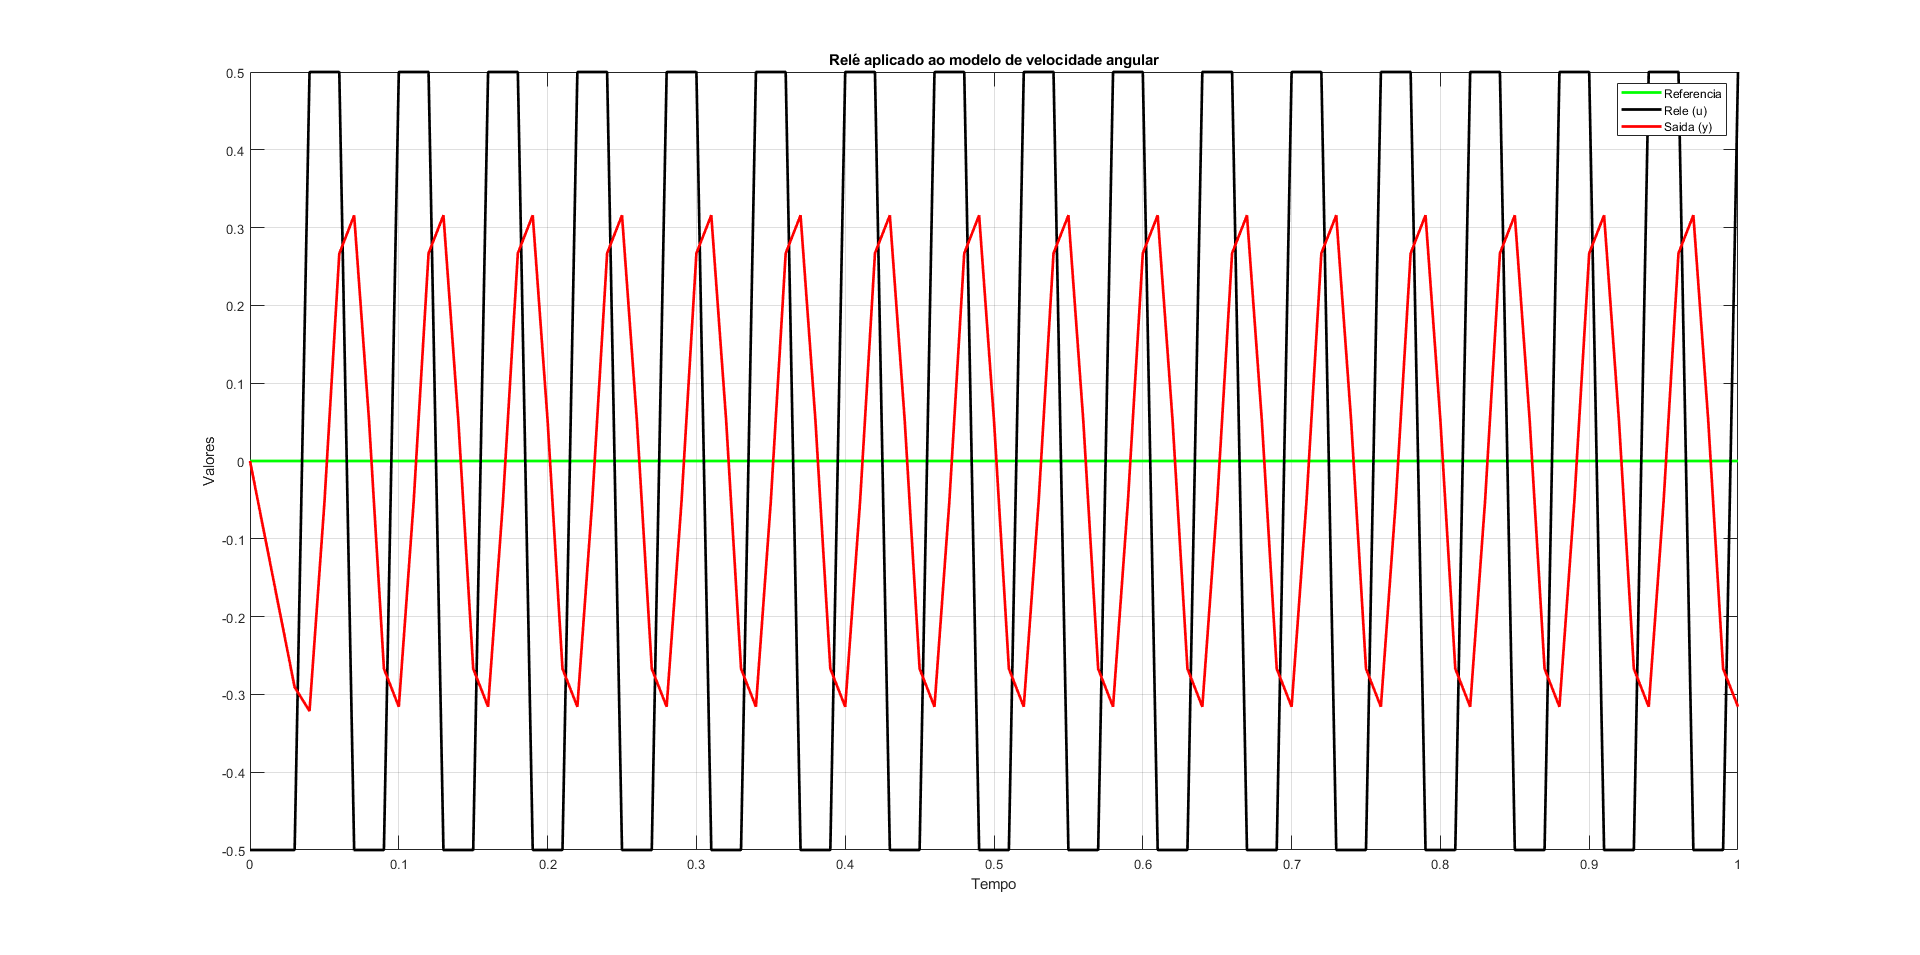
\includegraphics[width=16cm]{figuras/resultados/fig-global/rele-w-ang.png}
                    }{
                        \Fonte{O autor}
                    }	
            \end{figure}

            \begin{table}[!htbp]	
				\centering
				\Caption{\label{tab:parametros-rele-global} Parâmetros do Relé para as malhas globais}
				\UFCtab{}{
					\begin{tabular}{ccc}
						\toprule
						    Parâmetro/Malha & \( V \) & \( \omega \) \\
						\midrule
                            \( K_{u} \) & \( 5.2831 \) & \( 2.0111 \) \\
                            \( T_{u} \)    & \( 0.0600 \) & \( 0.0600 \) \\
                            \( a \)   & \( 0.1205 \) & \( 0.3165 \) \\
                            \( d \)   & \( 0.5000 \) & \( 0.5000 \) \\
                            \( \epsilon \)   & \( 0.1 \) & \( 0.29  00 \) \\
                            \( \omega_{u} \)   & \( 104.7198 \) & \( 104.7198 \) \\
						\bottomrule
					\end{tabular}
				}{
					\Fonte{O autor}
				}
			\end{table}

            No presente trabalho, por questões de limitações temporais, associadas, também, a problemas técnicos encontrados nas etapas práticas finais, não foi possível realizar a implementação prática das malhas de controle globais como foi feito com os controladores dos motores, de forma que para estas malhas estão apresentadas resultados simulados, os quais permitem ter uma compreensão de como se dará o comportamento do robô quando aplicado em condições de teste reais.

            Novamente, e de forma semelhante ao que foi apresentado para os controladores dos motores direito e esquerdo os controladores projetados são avaliados em ensaios para um e para três patamares. Os parâmetros dos controladores são apresentados na Tabela \ref{tab:parametros-controladores-global}.

            \begin{table}[!htbp]	
				\centering
				\Caption{\label{tab:parametros-controladores-global} Parâmetros dos Controladores Supervisórios}
				\UFCtab{}{
					\begin{tabular}{ccc}
						\toprule
						Parâmetro/Malha & \( V \) & \( \omega \) \\
						\midrule
						\( g_0 \) & \( 0.5839 \) & \( 1.6144 \) \\
						\( g_1 \)    & \( -0.5913 \) & \( -1.2420 \) \\
						\( g_2 \)   & \( 0.1700 \) & \( 0.3219 \) \\
						\bottomrule
					\end{tabular}
				}{
					\Fonte{O autor}
				}
			\end{table}

            Nas Figuras \ref{fig:controle-vel-linear-1-patamar} e \ref{fig:controle-w-ang-1-patamar} são apresentados os resultados dos ensaios simulados para um patamar de referência e na Tabela \ref{tab:metricas-pid-global-1-patamar} as métricas obtidas nesta situação. Para a malha de $\omega$ manteve-se a referência como sendo $\frac{\pi}{2}$ enquanto para a de $V$ a referência foi de $50\%$. Em seguida são realizados ensaios para 3 patamares e os resultados obtidos são apresentados nas Figuras \ref{fig:controle-vel-linear-3-patamar} e \ref{fig:controle-w-ang-3-patamar} bem como as métricas estão sintetizadas na Tabela \ref{tab:metricas-pid-global-3-patamar}.

            \begin{figure}[htbp]
                \centering
                \Caption{\label{fig:controle-vel-linear-1-patamar} Controle de $V$ para 1 patamar}	
                    \UFCfig{}{
                        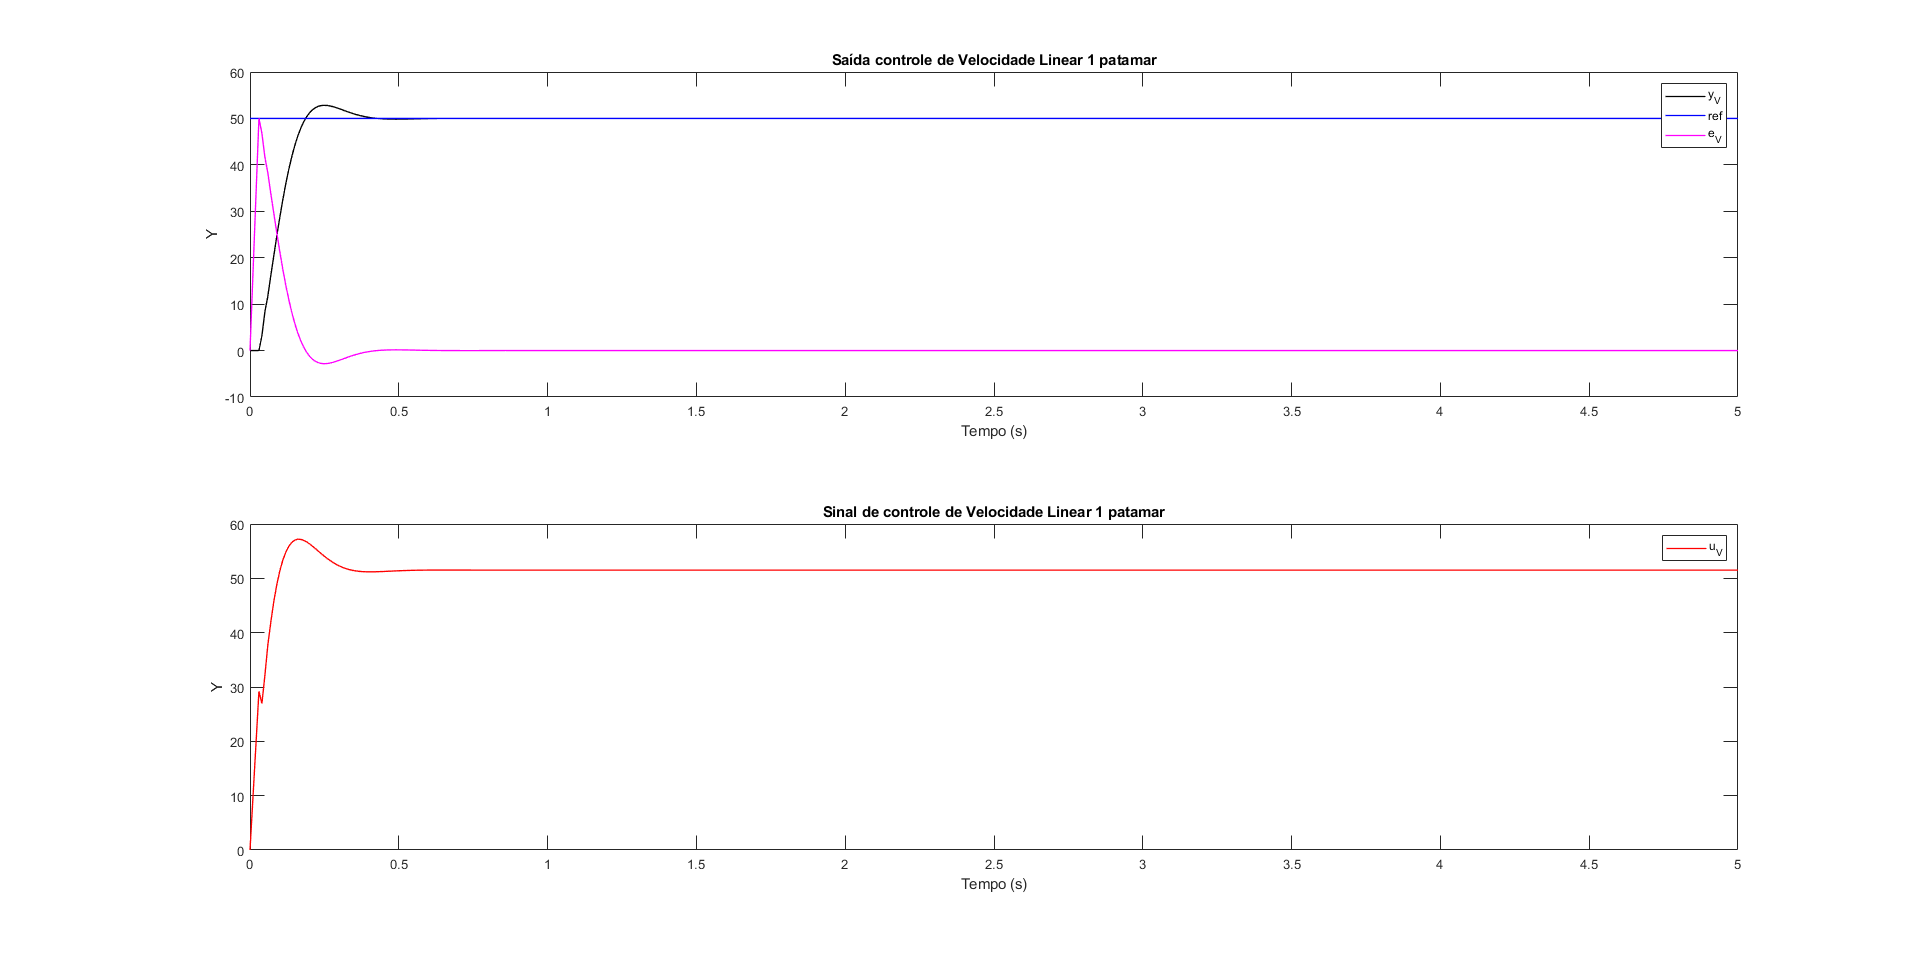
\includegraphics[width=16cm]{figuras/resultados/fig-global/contrtole-vel-lin-1-patamar.png}
                    }{
                        \Fonte{O autor}
                    }	
            \end{figure}

            \begin{figure}[htbp]
                \centering
                \Caption{\label{fig:controle-w-ang-1-patamar} Controle de $\omega$ para 1 patamar}	
                    \UFCfig{}{
                        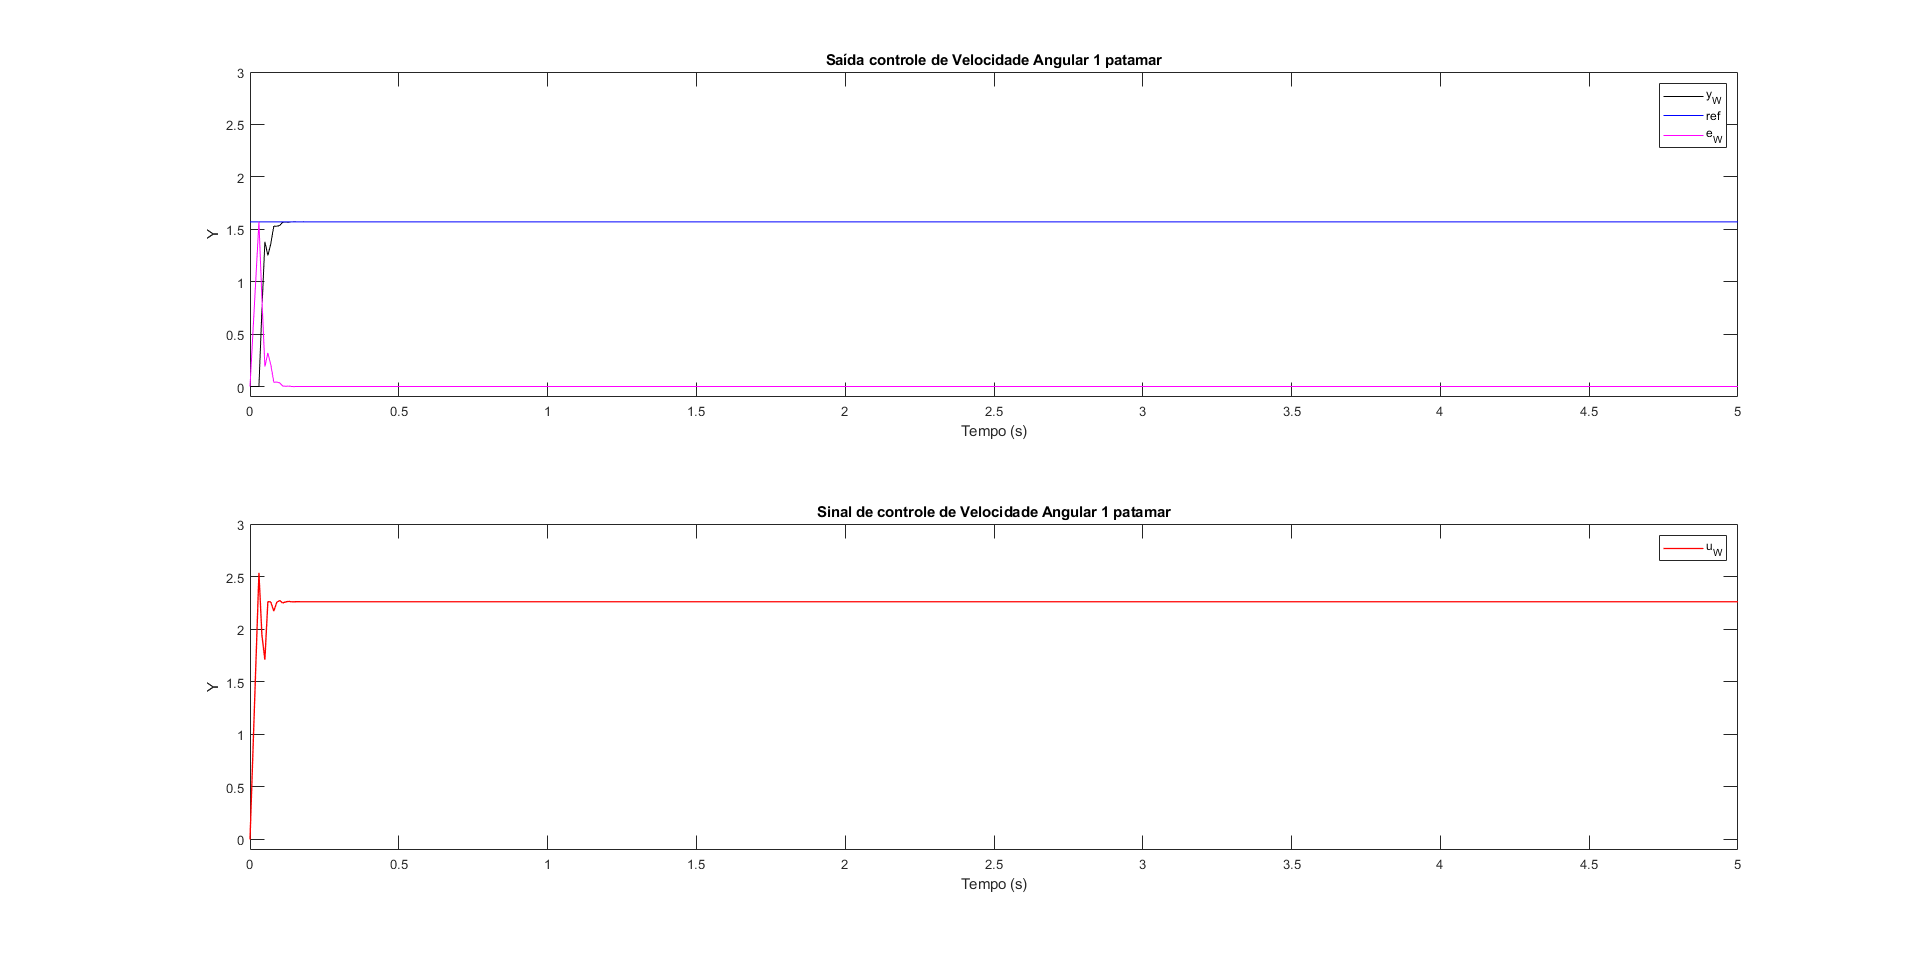
\includegraphics[width=16cm]{figuras/resultados/fig-global/contrtole-w-ang-1-patamar.png}
                    }{
                        \Fonte{O autor}
                    }	
            \end{figure}

            \begin{table}[!htbp]	
				\centering
				\Caption{\label{tab:metricas-pid-global-1-patamar} Resultados de controle para 1 patamar de $V$ e $\omega$}
				\UFCtab{}{
					\begin{tabular}{ccc}
						\toprule
						    Métrica/Malha & \( V \) & \( \omega \) \\
						\midrule
                            Sobressinal (\%) & \( 5.6565 \) & \( 0.0388 \) \\
                            IAE & \( 388.8405 \) & \( 3.2586 \) \\
                            Variância da saída & \( 33.0502 \) & \( 0.0165 \) \\
                            Variância da do controle & \( 14.7844 \) & \( 0.0214 \) \\
                            Tempo de assentamento (s) & \( 0.3200 \) & \( 0.0700 \) \\
						\bottomrule
					\end{tabular}
				}{
					\Fonte{O autor}
				}
			\end{table}

            \begin{figure}[htbp]
                \centering
                \Caption{\label{fig:controle-vel-linear-3-patamar} Controle de $V$ para 3 patamares}	
                    \UFCfig{}{
                        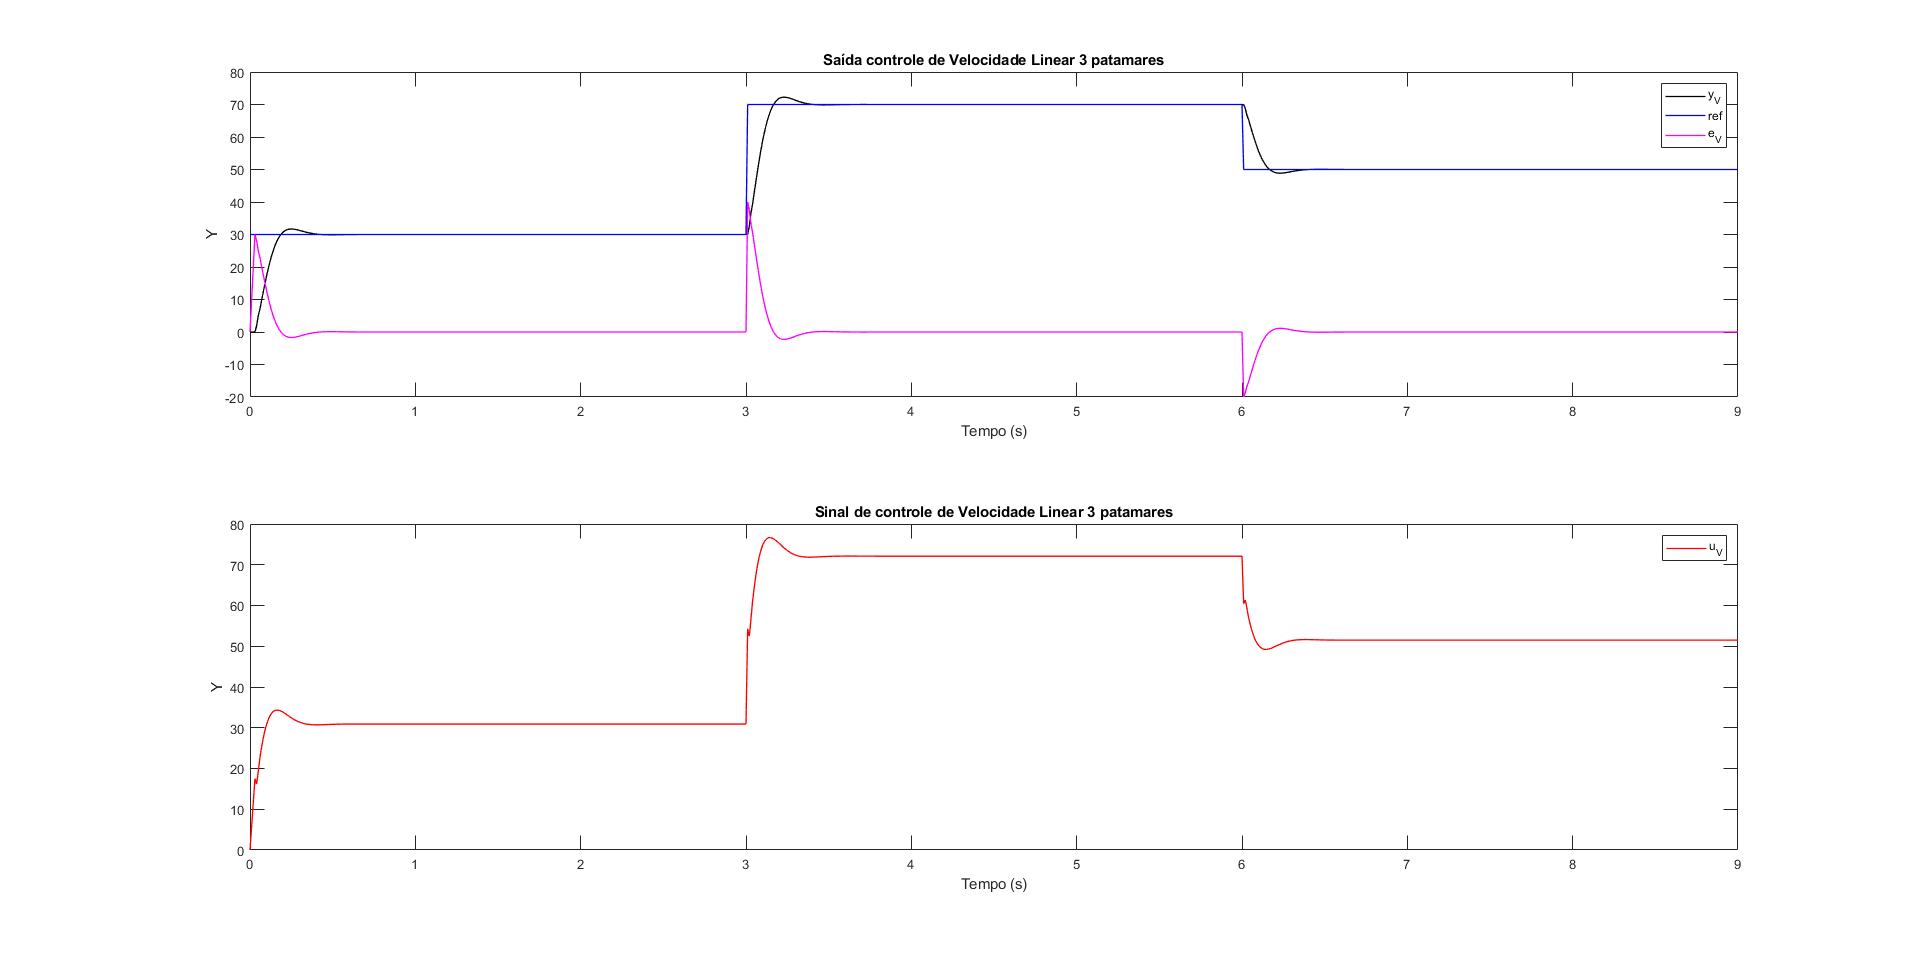
\includegraphics[width=16cm]{figuras/resultados/fig-global/contrtole-vel-lin-3-patamar.png}
                    }{
                        \Fonte{O autor}
                    }	
            \end{figure}

            \begin{figure}[htbp]
                \centering
                \Caption{\label{fig:controle-w-ang-3-patamar} Controle de $\omega$ para 3 patamares}	
                    \UFCfig{}{
                        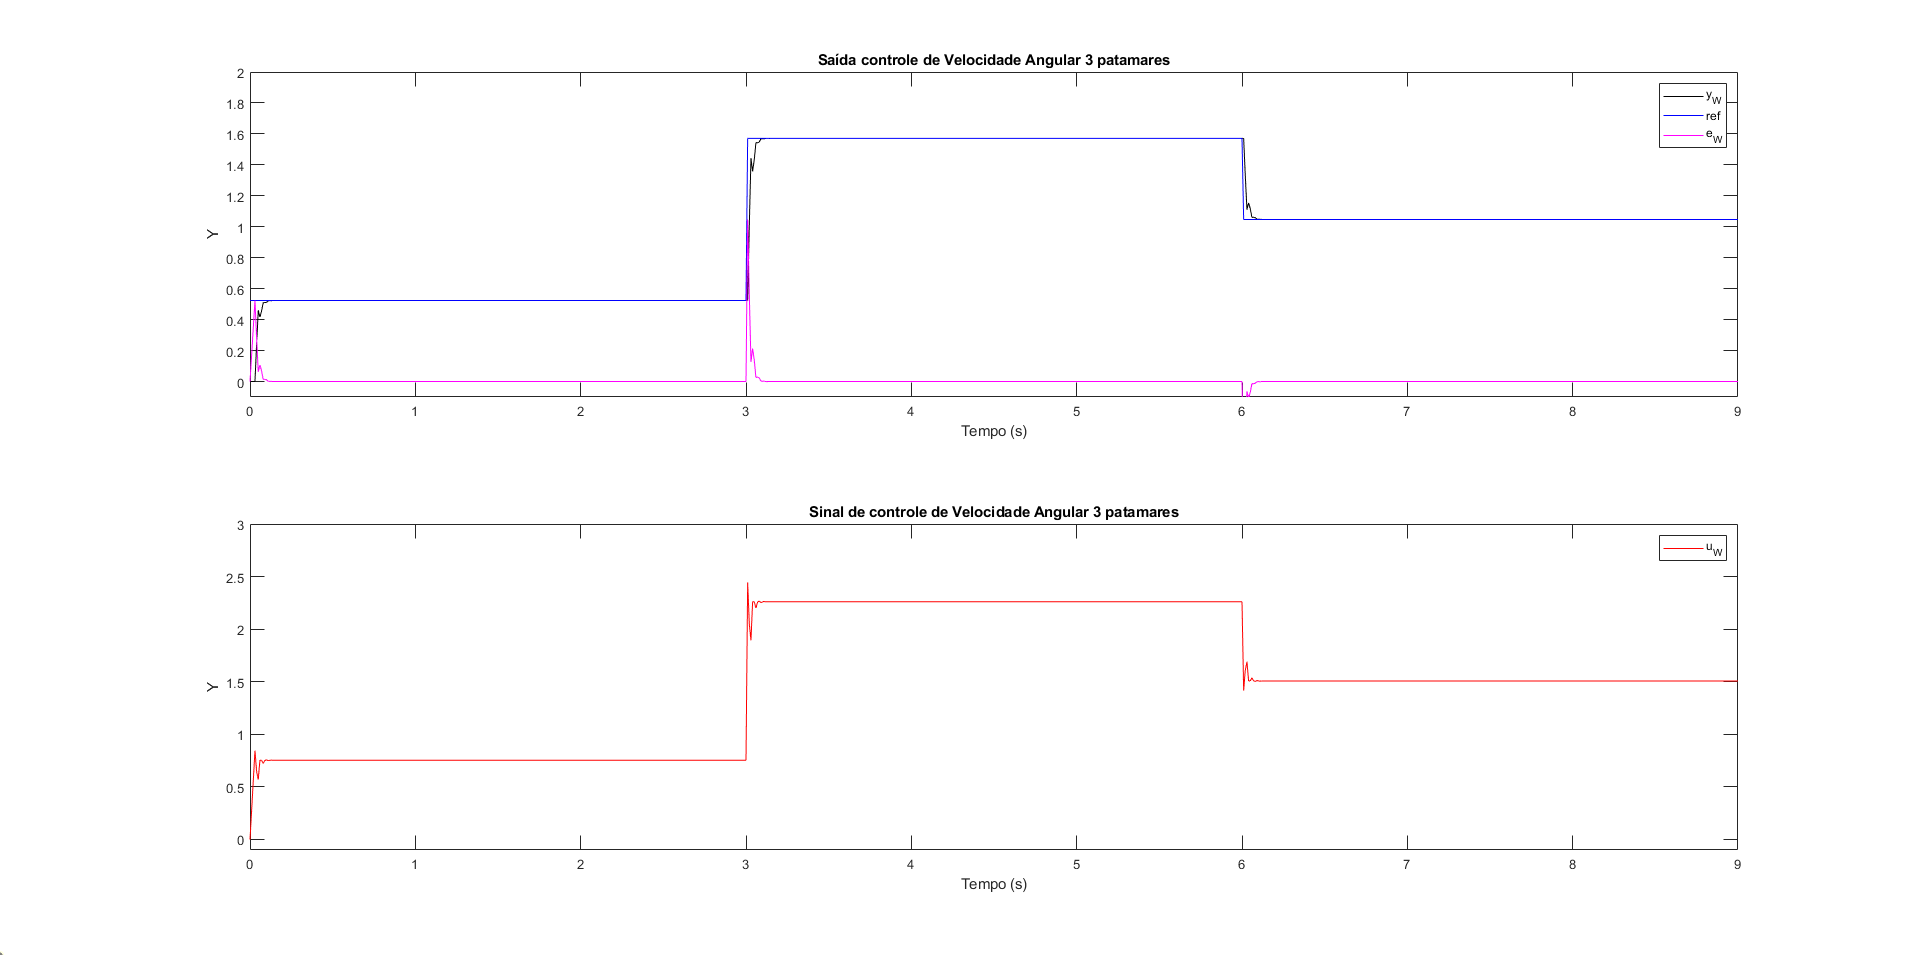
\includegraphics[width=16cm]{figuras/resultados/fig-global/contrtole-w-ang-3-patamar.png}
                    }{
                        \Fonte{O autor}
                    }	
            \end{figure}

            \begin{table}[!htbp]	
				\centering
				\Caption{\label{tab:metricas-pid-global-3-patamar} Resultados de controle supervisório para 3 patamares}
				\UFCtab{}{
					\begin{tabular}{ccc}
						\toprule
						    Métrica/Malha & \( V \) & \( \omega \) \\
						\midrule
                            Sobressinal do primeiro patamar (\%) & \( 5.6565 \) & \( 0.0388 \) \\
                            IAE & \( 699.9129 \) & \( 4.3449 \) \\
                            Variância da saída & \( 283.9178 \) & \( 0.1860 \) \\
                            Variância da do controle & \( 290.7013 \) & \( 0.3828 \) \\
                            Tempo de assentamento (s) do primeiro patamar & \( 0.3200 \) & \( 0.0500 \) \\
						\bottomrule
					\end{tabular}
				}{
					\Fonte{O autor}
				}
			\end{table}

            Tendo como ponto de análise as métricas obtidas para os controladores projetados para as malhas globais, é possível observar que o comportamento obtido encontra-se dentro do esperado haja vista que é possível interpretar as malhas globais ou supervisórias como um complemento e refino do controle realizado pelas malhas internas.
	\chapter{Conclusões e Trabalhos Futuros} \label{cap:conclusoes-e-trabalhos-futuros}

    A competição de robôs solucionadores de labirintos, os \textit{micromouses}, já é, há algum tempo, uma realidade consolidade dentro do cenário do estudo de robótica e controle em especial no cenário nacional haja vista seu caráter multidisciplinar no âmbito da Engenharia. E, dessa forma, o desenvolvimento de um robô para participação de competições do tipo é um trabalho relativamente complexo e muitas vezes realizado em equipe. Nesse contexto, o presente trabalho buscou abordar uma das etapas iniciais nesse desenvolviment, isto é, a etapa de controle das velocidades do robô.

    Tendo em vista a metodologia desenvolvida no que se refere à comunicação sem fio, pode-se concluir que esta demonstrou-se adequada dentro do cenário do Laboratório de Controle e Automação do grupo \gls{GRASI} do curso de Engenharia Elétrica da \gls{UFPI}, uma vez que as coletas de dados e a identificação evidenciaram um correto funcionamento da telemetria. Além disso, a comunicação sem fio mostrou-se compatível com a natureza móvel do robô, permitindo a execução de testes sem a utilização de conexões físicas que pudessem restringir seu deslocamento. Dessa forma, foi possível realizar experimentos em superfícies e condições de operação mais próximas daquelas encontradas em ambientes de competição.

    Já no referente à metodologia adotada para o projeto de controladores é possível observar, para os controladores dos motores, que, apesar de ruídos de medição que possam aparecer no processo ou de não-linearidades não modeladas, os motores mantiveram suas velocidades estáveis e controaldas, seguindo as diversas referências testadas. Quanto aos controladores supervisórios os resultados apresentados levam a crer que, com o desacoplamento inserido devido à utilização de malhas internas, o comportamento do robô também se manterá estável se realizados testes em condições reais.

    % Assim, conclui-se que o robô micromouse, apesar da sua complexidade, pode ser, de maneira relativamente fácil, adequadamente controlado quando em condições adequadas de testagem e dispondo de meios confiáveis para a transmissão das informações obtidas.

    Diante dos resultados apresentados, conclui-se que os objetivos relacionados à aquisição de dados, à identificação dos sistemas e ao projeto dos controladores de velocidade foram alcançados nas condições experimentais consideradas. A estrutura desenvolvida possibilitou o controle individual dos motores e estabeleceu uma base para o controle das variáveis globais de movimento do \textit{micromouse}. 
    
    Assim, o trabalho apresenta-se como um passo importante para as etapas posteriores de desenvolvimento da plataforma, especialmente aquelas relacionadas à navegação autônoma e à resolução de labirintos.

    Para trabalhos futuros, e de posse da estrutura já desenvolvida, sugere-se abordar o desenvolvimento de algorítmos de rastreio de trajetórias com e sem o uso de sistemas externos de visão, tais quais câmeras. Tais algorítmos serviriam de base ainda, para o entendimento e elaboração de algoritmos de resolução de labirintos como o algoritmo \textit{Flood Fill}.

    









	%Elementos pós-textuais	
	\bibliography{elementos-pos-textuais/referencias}
	% \imprimirglossario	
	\imprimirapendices
		% Adicione aqui os apendices do seu trabalho
		% \apendice{Código em Arduino do ESP32 DEVKIT V1}
\label{ap:devkit-v1}

\lstinputlisting[language=C++]{DEVKIT_SEND_RECEIVE.ino}


		% \apendice{Código em Arduino do ESP32 WEMOS D1 R32}
\label{ap:wemos}

\lstinputlisting[language=C++]{WEMOS_SEND_RECEIVE.ino}
        % \apendice{Comandos do MATLAB}
\label{ap:matlab}

\lstinputlisting[language=Matlab]{compilado.m}

	%\imprimiranexos
		% Adicione aqui os anexos do seu trabalho
		% \anexo{Exemplo de Anexo}
\label{an:exemplo-de-anexo}

Texto texto texto texto texto texto texto  texto texto texto  texto texto texto  texto texto texto  texto texto texto  texto texto texto  texto texto texto  texto texto texto  texto texto texto  texto texto texto  texto texto texto. 		
		% \anexo{Titulo anexo}
\label{an:anexo_b}

Texto texto texto texto texto texto texto texto texto texto texto.

	\imprimirindice

\end{document}